%%%%%%%%%%%%%%%%%%%%%%%%%%%%%%%%%%%%%%%%%
% Masters/Doctoral Thesis 
% LaTeX Template
% Version 2.5 (27/8/17)
%
% This template was downloaded from:
% http://www.LaTeXTemplates.com
%
% Version 2.x major modifications by:
% Vel (vel@latextemplates.com)
%
% This template is based on a template by:
% Stehttps://www.overleaf.com/project/5eaae1a203484700016123c4ve Gunn (http://users.ecs.soton.ac.uk/srg/softwaretools/document/templates/)
% Sunil Patel (http://www.sunilpatel.co.uk/thesis-template/)
%
% Template license:
% CC BY-NC-SA 3.0 (http://creativecommons.org/licenses/by-nc-sa/3.0/)
%
%%%%%%%%%%%%%%%%%%%%%%%%%%%%%%%%%%%%%%%%%

%----------------------------------------------------------------------------------------
%	PACKAGES AND OTHER DOCUMENT CONFIGURATIONS
%----------------------------------------------------------------------------------------

\documentclass[
11pt, % The default document font size, options: 10pt, 11pt, 12pt
%oneside, % Two side (alternating margins) for binding by default, uncomment to switch to one side
spanish, % ngerman for German
singlespacing, % Single line spacing, alternatives: onehalfspacing or doublespacing
%draft, % Uncomment to enable draft mode (no pictures, no links, overfull hboxes indicated)
%nolistspacing, % If the document is onehalfspacing or doublespacing, uncomment this to set spacing in lists to single
%liststotoc, % Uncomment to add the list of figures/tables/etc to the table of contents
%toctotoc, % Uncomment to add the main table of contents to the table of contents
%parskip, % Uncomment to add space between paragraphs
%nohyperref, % Uncomment to not load the hyperref package
headsepline, % Uncomment to get a line under the header
% chapterinoneline, % Uncomment to place the chapter title next to the number on one line
% consistentlayout, % Uncomment to change the layout of the declaration, abstract and acknowledgements pages to \textit{match} the default layout
]{MastersDoctoralThesis} % The class file specifying the document structure
\usepackage{enumerate}
\usepackage{amsmath}
\usepackage[utf8]{inputenc} % Required for inputting international characters
\usepackage[T1]{fontenc} % Output font encoding for international characters
\usepackage{comment}
\usepackage{mathpazo} % Use the Palatino font by default
\usepackage{graphicx}
\usepackage{graphicx, wrapfig}
%\usepackage[backend=bibtex,bibencoding=ascii,style=numeric,natbib=true]{biblatex} % Use the bibtex backend with the authoryear citation style (which resembles APA)
% Pseudocódigo -----------------------------------------
\usepackage{algorithm}
\usepackage[noend]{algpseudocode}
\renewcommand{\algorithmicrequire}{\textbf{Input:}}
\renewcommand{\algorithmicensure}{\textbf{Output:}}

\usepackage[]{biblatex}
\usepackage{longtable}
\usepackage[table]{xcolor}
\usepackage{subfig}
\usepackage{pdflscape}
\usepackage{array}
\usepackage{marginnote}
\newcolumntype{P}[1]{>{\centering\arraybackslash}p{#1}}

\addbibresource{sample.bib}


\usepackage[autostyle=true]{csquotes} % Required to generate language-dependent quotes in the bibliography
\usepackage{float}
% \usepackage{tabu}
\usepackage{booktabs}
% \usepackage[table,xcdraw]{xcolor}
\renewcommand*{\lstlistingname}{Código}
%----------------------------------------------------------------------------------------
%	MARGIN SETTINGS
%----------------------------------------------------------------------------------------

\geometry{
	paper=a4paper, % Change to letterpaper for US letter
	outer=2.5cm, % Inner margin
	inner=3.8cm, % Outer margin
	bindingoffset=.5cm, % Binding offset
	top=1.5cm, % Top margin
	bottom=1.5cm, % Bottom margin
	%showframe, % Uncomment to show how the type block is set on the page
}

%----------------------------------------------------------------------------------------
%	THESIS INFORMATION
%----------------------------------------------------------------------------------------

\thesistitle{Determinación automática del control de una Red de Petri} % Your thesis title, this is used in the title and abstract, print it elsewhere with \ttitle
\supervisor{Ph.D. Ing {Micolini}, Orlando} % Your supervisor's name, this is used in the title page, print it elsewhere with \supname
\examiner{Ing. {Ventre}, Luis Orlando} % Your examiner's name, this is not currently used anywhere in the template, print it elsewhere with \examname
% \degree{Doctor of Philosophy} % Your degree name, this is used in the title page and abstract, print it elsewhere with \degreename

\authorA{\textsc{Izquierdo}, Agustina Nahir}
\matriculaA{37729473}
\emailA{agustina.izquierdo@mi.unc.edu.ar}

\authorB{\textsc{Navarro}, Matias Alejandro}
\matriculaB{38730347}
\emailB{matias.navarro@mi.unc.edu.ar}

\authorC{\textsc{Salvatierra}, Andrés}
\matriculaC{39611008}
\emailC{andressalvatierra@mi.unc.edu.ar}
% Your name, this is used in the title page and abstract, print it elsewhere with \authorname
% \addresses{} % Your address, this is not currently used anywhere in the template, print it elsewhere with \addressname

% \subject{Biological Sciences} % Your subject area, this is not currently used anywhere in the template, print it elsewhere with \subjectname

\university{Universidad Nacional de Córdoba} % Your university's name and URL, this is used in the title page and abstract, print it elsewhere with \univname
% \department{Facultad de Ciencias Exactas Físicas y Naturales} % Your department's name and URL, this is used in the title page and abstract, print it elsewhere with \deptname
% \group{\href{http://researchgroup.university.com}{Research Group Name}} % Your research group's name and URL, this is used in the title page, print it elsewhere with \groupname
\faculty{Facultad de Ciencias Exactas Físicas y Naturales} % Your faculty's name and URL, this is used in the title page and abstract, print it elsewhere with \facname

\AtBeginDocument{
\hypersetup{pdftitle=\ttitle} % Set the PDF's title to your title
\hypersetup{pdfauthor=\authornameA} % Set the PDF's author to your name
\hypersetup{pdfkeywords=\keywordnames} % Set the PDF's keywords to your keywords
}

\begin{document}

\frontmatter % Use roman page numbering style (i, ii, iii, iv...) for the pre-content pages

\pagestyle{plain} % Default to the plain heading style until the thesis style is called for the body content

%----------------------------------------------------------------------------------------
%	TITLE PAGE
%----------------------------------------------------------------------------------------

\begin{titlepage}
	\begin{center}
				
		\resizebox{0.9\textwidth}{!}{
\includegraphics{Figures/logo-unc-fcefyn.png}}%
				
		\vspace*{.06\textheight}
		{\scshape\LARGE \univname\par}\vspace{0.5cm} % University name
		{\scshape\LARGE \facname\par}\vspace{1cm}
		\textsc{\Large Proyecto Integrador}\\[0.5cm] % Thesis type
		\textsc{\Large Ingeniería en Computación}\\[0.5cm]
				
		\HRule \\[0.4cm] % Horizontal line
		{\huge \bfseries \ttitle\par}\vspace{0.3cm} % Thesis title
		\HRule \\[1.5cm] % Horizontal line
				 
		\begin{minipage}[t]{0.5\textwidth}
			\begin{flushleft} \large
				\emph{Autores:}\\
				\authornameA \\ % Author name - remove the \href bracket to remove the link
				\matriculanameA \\
				\emailnameA \\
				\hfill \break
				\authornameB \\
				\matriculanameB \\
				\emailnameB \\
				\hfill \break
				\authornameC \\
				\matriculanameC \\
				\emailnameC \\
				
			\end{flushleft}		
		\end{minipage}
		\begin{minipage}[t]{0.4\textwidth}
			\begin{flushright} \large
				\emph{Director:} \\
				\supname \\
				\hfill \break
				\emph{Co-director:} \\
				\examname
			\end{flushright}
		\end{minipage}\\[2cm]
				
		% \large \textit{A thesis submitted in fulfillment of the requirements\\ for the degree of \degreename}\\[0.3cm] % University requirement text
		% \textit{in the}\\[0.4cm]
		% \groupname\\\deptname\\[2cm] % Research group name and department name
				
		{\large {Noviembre 2020}}\\[4cm] % Date
		%\includegraphics{Logo} % University/department logo - uncomment to place it
				 
		\vfill
	\end{center}
\end{titlepage}

%----------------------------------------------------------------------------------------
%	DEDICATION
%----------------------------------------------------------------------------------------

% \dedicatory{Para nuestras familias\ldots} 

% %----------------------------------------------------------------------------------------
% %	DECLARATION PAGE
% %----------------------------------------------------------------------------------------

% \begin{declaration}
% \addchaptertocentry{\authorshipname} % Add the declaration to the table of contents
% \noindent I, \authorname, declare that this thesis titled, \enquote{\ttitle} and the work presented in it are my own. I confirm that:

% \begin{itemize} 
% \item This work was done wholly or mainly while in candidature for a research degree at this University.
% \item Where any part of this thesis has previously been submitted for a degree or any other qualification at this University or any other institution, this has been clearly stated.
% \item Where I have consulted the published work of others, this is always clearly attributed.
% \item Where I have quoted from the work of others, the source is always given. With the exception of such quotations, this thesis is entirely my own work.
% \item I have acknowledged all main sources of help.
% \item Where the thesis is based on work done by myself jointly with others, I have made clear exactly what was done by others and what I have contributed myself.\\
% \end{itemize}
 
% \noindent Signed:\\
% \rule[0.5em]{25em}{0.5pt} % This prints a line for the signature
 
% \noindent Date:\\
% \rule[0.5em]{25em}{0.5pt} % This prints a line to write the date
% \end{declaration}

% \cleardoublepage

%----------------------------------------------------------------------------------------
%	QUOTATION PAGE
%----------------------------------------------------------------------------------------

% \vspace*{0.2\textheight}

% \noindent\enquote{\itshape Thanks to my solid academic training, today I can write hundreds of words on virtually any topic without possessing a shred of information, which is how I got a good job in journalism.}\bigbreak

% \hfill Dave Barry

%----------------------------------------------------------------------------------------
%	ABSTRACT PAGE
%----------------------------------------------------------------------------------------

\begin{abstract}
	%\addchaptertocentry{\abstractname} % Add the abstract to the table of contents
    El contenido de este documento abarca las motivaciones, objetivos, detalles de implementación y demás datos pertinentes al desarrollo del Proyecto Integrador para la carrera de Ingeniería en Computación. El mismo se estructura en cuatro grandes partes: introducción del proyecto, marco teórico, desarrollo de la investigación, conclusiones obtenidas y trabajo a futuro.
    
    \par \noindent El tema a abarcar es principalmente el análisis de redes de Petri que presentan estados de deadlock, teniendo como objetivo desarrollar y documentar un algoritmo que permita el control de las mismas, restringiendo el alcance de estos estados.

\end{abstract}

% \textbf{Palabras Clave:} \textit{\keywordnames}

%----------------------------------------------------------------------------------------
%	ACKNOWLEDGEMENTS
%----------------------------------------------------------------------------------------
 
\begin{acknowledgements}
	
	\addchaptertocentry{\acknowledgementname} % Add the acknowledgements to the table of contents

	% 	{\normalsize familiares y directores \par}
	Muchas gracias a nuestras familias, por el apoyo incondicional a lo largo de todos estos años de estudio. Este proyecto no hubiera sido posible sin el soporte, la confianza, la supervisión y el empeño de nuestros directores, \supname \ e \ \examname .
	\bigskip
			
	% 	{\normalsize amigos \par}
	Un especial agradecimiento a nuestros amigos y todas las personas que tuvimos el placer de conocer durante estos años de carrera. 
	\bigskip
			
	% 	{\normalsize universisdad \par}
    Finalmente, agradecemos a la Facultad de Ciencias Exactas Físicas y Naturales de la Universidad Nacional de Córdoba por la oportunidad de realizar esta carrera de grado.
    
	\vspace*{\fill}
		
\end{acknowledgements}

%----------------------------------------------------------------------------------------
%	LIST OF CONTENTS/FIGURES/TABLES PAGES
%----------------------------------------------------------------------------------------

\hypersetup{
	linkcolor=black,
	citecolor=black,
	urlcolor=black
	}

\tableofcontents % Prints the main table of contents

\listoffigures % Prints the list of figures
\hfill
\textbf{Nota:} Todas las figuras que no presenten una referencia son de autoría propia. 

\listoftables % Prints the list of tables

%----------------------------------------------------------------------------------------
%	ABBREVIATIONS
%----------------------------------------------------------------------------------------

\begin{abbreviations}{ll} % Include a list of abbreviations (a table of two columns)

	\textbf{AMS} & \textbf{A}utomated \textbf{M}anufacturing \textbf{S}ystems. \\
	\textbf{FIFO} &\textbf{F}irst \textbf{I}n \textbf{F}irst \textbf{O}ut. \\
	\textbf{FMS} & \textbf{F}lexible \textbf{M}anufacturing \textbf{S}ystems\\
	\textbf{LAC} & \textbf{L}aboratorio de \textbf{A}rquitectura de \textbf{C}omputadoras \\
	\textbf{RdP} & \textbf{R}ed de \textbf{P}etri \\
	\textbf{RAS} & \textbf{R}esource \textbf{A}llocation \textbf{S}ystem\\
	\textbf{S³PR} & \textbf{S}ystem of \textbf{S}imple \textbf{S}equential \textbf{P}rocesses with \textbf{R}esources\\
	\textbf{WP} & \textbf{W}ork \textbf{P}rocess
	
	
\end{abbreviations}
%----------------------------------------------------------------------------------------
%	THESIS CONTENT - CHAPTERS
%----------------------------------------------------------------------------------------

\mainmatter % Begin numeric (1,2,3...) page numbering

\pagestyle{thesis} % Return the page headers back to the "thesis" style

% Include the chapters of the thesis as separate files from the Chapters folder
% Uncomment the lines as you write the chapters

 % Chapter Template

\chapter{Introducción} % Main chapter title

\label{Chapter1} % Change X to a consecutive number; for referencing this chapter elsewhere, use \ref{ChapterX}

\section{Motivación e importancia del proyecto}

Las motivaciones para el desarrollo de este trabajo pueden dividirse en dos grandes pilares. Por un lado aquellas relacionadas al proyecto en sí, entre las cuales puede destacarse la necesidad de realizar una investigación y desarrollo de un algoritmo capaz de solucionar los problemas de vivacidad de las redes de Petri(RdP), puntualmente las que modelan Sistemas de procesos secuenciales simples con recursos($S^3PR$). Sumado a que el mismo podría formar parte de un proyecto más robusto que se está desarrollando en el Laboratorio de Arquitectura de Computadoras, y esto es algo emocionante.
\bigskip 

Por otra parte, existen sin duda ciertas motivaciones de naturaleza académica. Entre ellas podemos mencionar la integración de los conocimientos adquiridos a lo largo de nuestros estudios, la contribución a la comunidad de investigadores e incluso la puesta en práctica de procedimientos estrictos de investigación, de desarrollo de software y de documentación que nos serán sin duda de gran valor durante nuestro futuro ejercicio como profesionales.

%----------------------------------------------------------------------
% Estado del Arte
%----------------------------------------------------------------------
\section{Estado del arte}

En 1962, Petri inventó un enfoque teórico de la red para modelar y analizar los sistemas de comunicación en su tesis \cite{petri1962kommunikation}. Este modelo se basó en los conceptos de funcionamiento asíncrono y concurrente de las partes de un sistema y en la comprensión de que las relaciones entre las partes podían representarse mediante una red. Se ha realizado una gran cantidad de investigaciones tanto sobre la naturaleza como sobre la aplicación de las redes de Petri, la cuál parece estar en expansión.\\
Se ha demostrado que las redes de Petri son muy útiles en el modelado, análisis, simulación y control de sistemas concurrentes.

\par El flujo simultáneo de varios procesos en un sistema de asignación de recursos (RAS), que compiten por un conjunto finito de recursos, puede conducir a un punto muerto. Un interbloqueo (deadlock) ocurre cuando un conjunto de procesos se encuentra en un estado de ``espera circular''\footnote{Definido en el Marco Teórico (Sección \ref{sec:Interbloqueo})}, donde cada proceso del conjunto está esperando que un recurso sea liberado por otro proceso del conjunto mientras ocupa un recurso que, a su vez, es necesario por uno de los otros procesos. La noción de deadlock parcial o total es frecuente y es preferible la validación antes de la implementación para reducir los riesgos \cite{LIU2016198}.

Los estado de deadlock son una situación bastante indeseable en un sistema de fabricación automatizado. Su ocurrencia a menudo deteriora la utilización de recursos y pueden conducir a resultados catastróficos en sistemas críticos para la seguridad. Las redes de Petri son una herramienta matemática importante para manejar problemas de interbloqueo en sistemas de asignación de recursos.

Un sistema de fabricación flexible (FMS) o un sistema de fabricación automatizado (AMS) son un conglomerado de máquinas herramienta controladas numéricamente por computadora, amortiguadores, accesorios, robots, vehículos guiados automatizados (AGV) y otros dispositivos de manejo de materiales. Por lo general, exhibe un alto grado de uso compartido de recursos para aumentar la flexibilidad. La existencia de recursos compartidos puede conducir a condiciones de espera circular. En tal sistema, una vez que ocurren los puntos muertos, persisten y no se resolverían sin la intervención de seres humanos u otro agente externo.

En diversos estudios realizados por distintos autores, en busca de reducir estos estados de deadlock, se parte de la premisa de la existencia de cuatro estrategias para manejarlos.

\subsection{Estrategias de manejo de deadlock}

\subsubsection{Ignorar (Deadlock ignoring)}
Ignorar los estados de deadlock, que se conoce como el algoritmo de Ostrich \footnote{Concepto informático para denominar el procedimiento de algunos sistemas operativos. Esta teoría, acuñada por A. S. Tanenbaum, señala que dichos sistemas, en lugar de enfrentar el problema de los bloqueos mutuos asumen que estos nunca ocurrirán.}, se emplea en un sistema de asignación de recursos si la probabilidad de que se produzcan puntos muertos es mínima y la aplicación de otras estrategias de control de deadlock es técnicamente difícil. En un FMS o AMS, ignorar el estado deadlock es factible y razonable desde el punto de vista técnico y económico si el grado de intercambio de recursos es bajo.

\subsubsection{Prevenir (Deadlock prevention)}
Se logra controlando la solicitud de recursos y garantizando que nunca se produzcan estados de deadlock. Los recursos se otorgan a los procesos de tal manera que una solicitud de un recurso nunca conduce a situaciones de deadlock. El objetivo es imponer limitaciones a la evolución de un sistema. En este caso, el calculo se realiza offline de forma estática y una vez establecida una política de control, el sistema ya no puede alcanzar esos estados indeseables.
Una ventaja importante de los algoritmos de prevención de interbloqueo es que no requieren ningún costo de tiempo de ejecución, ya que los problemas se resuelven en las etapas de diseño y planificación del sistema.La principal crítica es que tienden a ser demasiado conservadores, lo que reduce la utilización de recursos y la productividad del sistema.

\subsubsection{Evitar (Deadlock avoidance)}
Para evitar los estados de deadlock se concede un recurso a un proceso solo si el estado resultante es seguro. Un estado se denomina seguro si existe al menos una secuencia de ejecución que permite que todos los procesos se ejecuten hasta su finalización. Para decidir si el próximo estado es seguro si se asigna un recurso a un proceso se debe realizar un seguimiento del estado del sistema global. Esto significa que son necesarios un gran almacenamiento y una amplia capacidad de comunicación.

\subsubsection{Detectar y recuperar (Deadlock detection and recovery)}
Se otorgan recursos a un proceso sin ningún control. El estado de la asignación de recursos y las solicitudes se examinan periódicamente para determinar si un conjunto de procesos está bloqueado. Este examen se realiza mediante un algoritmo de detección de interbloqueo. Si se encuentra un interbloqueo, el sistema se recupera abortando uno o más procesos interbloqueados y entregandole los recursos liberados a otros procesos. En la práctica de fabricación, a menudo se necesitan operadores humanos para esta estrategia y, por lo tanto, puede resultar muy costoso.

\subsection{Revisión de la literatura}
Las políticas de prevención de deadlock se han logrado ampliamente y han dado lugar a una gran cantidad de resultados. En esta sección, se revisan las estrategias de \textbf{prevención} de deadlock mediante el uso de redes de Petri y se desarrollan en base a diferentes técnicas como el análisis estructural y el análisis del grafo de alcanzabilidad.

\subsubsection{Métodos de análisis estructural}
Ezpeleta et al. \cite{paperezpeleta} utilizó una clase de redes de Petri, las del tipo S³PR y propuso un algoritmo para la asignación de recursos en FMS. El algoritmo propuesto agregó nuevos lugares a la red para imponer ciertas restricciones que prohíben la presencia de sifones vacíos.

Los trabajos de Huang et al. \cite{YiShengBook} y Huang y et al. \cite{YHuangandJeng} presentan una nueva política de prevención de deadlock para la clase de redes de Petri, donde los estados de deadlock están relacionados con sifones sin marcar. Se agregan dos tipos de lugares de control al modelo original para un sistema de fabricación flexible llamado lugar de control ordinario y lugar de control ponderado para evitar que los sifones se desmarquen.

En Li y Wei \cite{LiandWei} , se introduce el concepto de sifones elementales para diseñar un supervisor de red de Petri que haga cumplir la vivacidad para el mismo modelo de red de Petri. Basado en sifones elementales y conceptos de P-invariantes en redes de Petri, Li y Wei introducen un algoritmo de prevención de interbloqueo para una clase específica de redes de Petri que pueden modelar adecuadamente varios FMS \cite{LiandWei}, los sifones en un modelo de red de Petri se clasifican en dependientes y sifones elementales, y se agregan lugares de control para todos los sifones elementales, de modo que los sifones están controlados de forma invariante.

Huang \cite{Huang2007} propone una nueva metodología para sintetizar supervisores para la asignación de recursos en los FMS; se considera la clase de red Petri, a saber, S³PR, donde los puntos muertos están relacionados con sifones mínimos no marcados; todos los sifones mínimos deben controlarse agregando plazas de control. En este estudio, el número de plazas de control se reduce utilizando el concepto de sifón elemental.

Chen et al. \cite{paperchen}, presenta un algoritmo de prevención de deadlock y el concepto de extracción por sifón se utiliza para calcular sifones no marcados para el modelo de red de Petri. Primero, un algoritmo de extracción de sifón obtiene un sifón no marcado máximo, divide los lugares en él y determina un sifón necesario de los lugares divididos; esto se lleva a cabo para todos los sifones sin marcar. Luego, el algoritmo diseña un monitor conveniente para marcar cada sifón necesario hasta que el modelo de red de Petri controlado esté activo.

Liu et al. \cite{LiuanLi2013} propuso una variedad de algoritmos de control de interbloqueo para AMS con recursos no confiables, los monitores y las subredes de recuperación están diseñadas para sifones mínimos estrictos (sifón vacío) y recursos no confiables, respectivamente, y se utilizan dos tipos de arcos que son normales e inhibidores para conectar monitores con subredes de recuperación. Para obtener un supervisor con complejidad estructural, los sifones elementales extraídos de todos los sifones mínimos estrictos están obviamente controlados. 


\subsubsection{Enfoques basados en el grafo de alcanzabilidad}
Viswanadham et al. \cite{Viswanadham} presentó métodos de asignación de recursos estáticos para eliminar los puntos muertos; En este estudio, se utiliza un grafo de alcanzabilidad del modelo de red de Petri para llegar al método de asignación de recursos estático. Se implementa un algoritmo de prevención de interbloqueo para un sistema de fabricación de tamaño pequeño que consta de una máquina y un vehículo guiado automatizado (AGV). Los autores observaron que el algoritmo propuesto se puede aplicar de manera efectiva sólo para sistemas de fabricación de tamaño pequeño.

\par El trabajo de Uzam \cite{uzam2004, uzam2002} propone y mejora el método basado en una teoría de regiones para diseñar un supervisor de red de Petri óptimo. El tamaño del grafo de alcanzabilidad del modelo de red de Petri es un problema importante para aplicar la política de prevención de interbloqueos a un modelo de red de Petri muy grande. Por lo tanto, propusieron un algoritmo de reducción para simplificar modelos de redes de Petri muy grandes con el fin de facilitar los cálculos necesarios. Basado en la teoría de las regiones, Uzam y Zhou \cite{uzamandzhou2004} desarrollaron una política iterativa de prevención de interbloqueos para FMS. En su estudio, el grafo de alcanzabilidad de un modelo de red de Petri se divide en dos partes: zona libre de bloqueo (zona activa, LZ) y zona de bloqueo (DZ). La zona viva se desarrolla ya que el componente máximo fuertemente conectado contiene la marca inicial. La zona de interbloqueo contiene marcas desde las que no se puede alcanzar la marca inicial. FBM está definido como una marca en la zona de interbloqueo. Los interbloqueos se pueden eliminar prohibiendo el disparo de las transiciones habilitadas en FBM. En su trabajo, el enfoque presentado tiene dos problemas. Primero, no se puede garantizar un supervisor óptimo en general, incluso si existe un supervisor óptimo. En segundo lugar, en cada iteración se requiere el cálculo del grafo de alcanzabilidad total para verificar si las marcas en la zona de interbloqueo son accesibles. Este enfoque es fácil de usar y simple si el grafo de alcanzabilidad de un sistema es pequeño pero no puede garantizar la optimización del comportamiento del supervisor. Los monitores redundantes en el supervisor de red de Petri pueden existir cuando el supervisor está diseñado mediante un enfoque de control de sifón iterativo. Por tanto, Uzam et al. \cite{uzammuratli2007} introdujo un enfoque para identificar y eliminar los monitores redundantes mediante el cálculo del gráfico de accesibilidad de un modelo de red de Petri controlado. Si la red de Petri controlada no pierde la vivacidad cuando se eliminan los monitores redundantes, entonces los monitores redundantes se pueden eliminar del supervisor.\\

El objetivo de esta sección fue presentar una revisión de la literatura sobre los distintos enfoques planteados hasta el momento respecto a la prevención de los estados de deadlock.
Un enfoque híbrido de control de interbloqueos se refiere a aquel que combina distintas de estas planificaciones para tratarlos. La motivación esencial de plantear una estrategia de este tipo es aprovechar las ventajas o formalismos de múltiples de estas, evitando sus desventajas. Esto fue puntualmente lo que nos motivó a no regirnos por una única estrategia o estudio planteado.


%----------------------------------------------------------------------
% Objetivos
%----------------------------------------------------------------------
\section{Objetivos}
Como se anticipó en la motivación, el objetivo final es el desarrollo de un algoritmo capaz de determinar las plazas y arcos necesarios a incorporar a la red original para lograr la ejecución de manera controlada, alcanzando la vivacidad de la misma. 

Al tratarse de un trabajo de investigación en el cual se fue evolucionando sobre distintas situaciones que se fueron encontrando a lo largo de su desarrollo, fueron apareciendo diferentes objetivos intermedios (mencionados en las diferentes iteraciones del mismo) mediante los que se logró alcanzar el objetivo principal antes mencionado que es obtener una red viva o libre de deadlock(interbloqueo).

\bigskip

Para esto se propone usar como soporte el software Petrinator, el mismo se utilizará para simular la redes y extraer la información necesaria de las mismas. Para que esta última pueda ser utilizada por nuestro algoritmo se proponen los siguientes objetivos secundarios:

\begin{itemize}
    \item Implementar una interfaz que procese la información extraída del software antes mencionado.
    
    \item Realizar una segunda interfaz que conecta el algoritmo nuevamente con el software Petrinator, indicando mediante una retroalimentación los nuevos arcos y plazas a colocar.
\end{itemize}

%----------------------------------------------------------------------
% Requerimientos
%----------------------------------------------------------------------
\section{Requerimientos}
En la ingeniería, los requerimientos se utilizan como datos de entrada en la etapa de diseño del producto. Establecen qué debe hacer el sistema, aunque no especifican la manera en que debe hacerlo. La fase de captura y registro de requisitos puede estar precedida por una fase de análisis conceptual del proyecto. 
\bigskip

\subsection{Listado de requerimientos}
\begin{table}[H]
    \centering
    \begin{tabular}{|c|p{12.8cm}|}
    \hline
    \textbf{ID} & \textbf{Descripción}  \\  \hline
    $R_{1}$ & Se debe usar el software Petrinator para la construcción, análisis y extracción de los archivos necesarios de la red de Petri.\\
    \hline
    
    $R_{2}$ & El algoritmo debe ser capaz de leer los archivos de extensión '.html' de los diferentes análisis exportados del Petrinator y llevar a cabo su posterior procesamiento para su utilización. \\ 
    \hline
    
    $R_{3}$ & El algoritmo debe modificar el archivo de extensión '.pflow' de la red en cuestión, para agregar plazas, arcos y quitar estos últimos en caso de ser necesario.\\
    \hline
    
    $R_{4}$ & Se debe agregar una funcionalidad al Petrinator para poder recargar la red una vez modificada por el algoritmo. \\ 
    \hline
    
    $R_{5}$ & El algoritmo debe converger en redes de Petri del tipo S³PR.  \\ 
    \hline
    
    $R_{6}$ & El algoritmo debe ser desarrollado para poder ser integrado al Petrinator como una nueva funcionalidad del mismo.  \\ 
    \hline
    
    \end{tabular}
    \label{tab:listadoRiesgos}
    \caption{Listado de requerimientos.}
\end{table}

%--------
% Riesgos
%--------
\section{Análisis de riesgos}
Un riesgo es un evento o condición incierta que, en caso de ocurrir, tendrá consecuencias negativas sobre al menos uno de los requerimientos del proyecto. Por esta razón es importante identificarlos con anticipación para mitigarlos.

\subsection{Listado de riesgos}
\begin{table}[H]
    \centering
    \begin{tabular}{|c|p{12.8cm}|}
    \hline
    \textbf{ID} & \textbf{Descripción}  \\  \hline
    $R_{1}$ & Recursos de hardware insuficientes.\\
    \hline
    
    $R_{2}$ & Ausencia de algoritmo. \\ 
    \hline
    
    $R_{3}$ & Algoritmo inadecuado. \\
    \hline
    
    $R_{4}$ & Herramienta inadecuada. \\ 
    \hline
    
    $R_{5}$ & Ausencia/escasez de datos. \\ 
    \hline
    
    \end{tabular}
    \label{tab:listadoRiesgos}
    \caption{Listado de riesgos.}
\end{table}

%--------
% R1
%--------
\begin{table}[H]
    \centering
    \begin{tabular}{|p{13.7cm}|}
    \hline
    \textbf{R1 - Recurso de hardware insuficiente} \\
    \hline \hline 
    \textbf{Condición}: Los recursos de hardware disponibles (computador básico) son inferiores a los necesarios.\\
    \hline
    \textbf{Consecuencia}: No permite analizar redes de Petri demasiado complejas, es decir, que presentan un gran numero de estados. \\
    \hline
    \textbf{Efecto}: Limitar la implementación de nuestro algoritmo a redes con una cantidad reducida de estados. \\
    \hline
    \end{tabular}
    \label{tab:R1}
    \caption{R1 - Recurso de hardware insuficiente.}
\end{table}

%--------
% R2
%--------
\begin{table}[H]
    \centering
    \begin{tabular}{|p{13.7cm}|}
    \hline
    \textbf{R2 - Ausencia de algoritmo} \\
    \hline \hline
    \textbf{Condición}: Inexistencia del algoritmo.\\
    \hline
    \textbf{Consecuencia}: No lograr alcanzar la vivacidad de una red de Petri. \\
    \hline
    \textbf{Efecto}: Irrealizabilidad del proyecto. \\
    \hline
    \end{tabular}
    \label{tab:R2}
    \caption{R2 - Ausencia de algoritmo.}
\end{table}

%--------
% R3
%--------
\begin{table}[H]
    \centering
    \begin{tabular}{|p{13.7cm}|}
    \hline
    \textbf{R3 - Algoritmo inadecuado} \\
    \hline \hline 
    \textbf{Condición}: Encontrar un algoritmo pero que no converge en todas las redes del mismo tipo.\\
    \hline
    \textbf{Consecuencia}: Iteraciones infinitas del algoritmo. \\
    \hline
    \textbf{Efecto}: Incremento del tiempo dedicado en la investigación para la readaptación del algoritmo. \\
    \hline
    \end{tabular}
    \label{tab:R3}
    \caption{R3 - Algoritmo inadecuado.}
\end{table}

%--------
% R4
%--------
\begin{table}[H]
    \centering
    \begin{tabular}{|p{13.7cm}|}
    \hline
    \textbf{R4 - Herramienta inadecuada} \\
    \hline \hline 
    \textbf{Condición}: Elección incorrecta de la herramienta para implementar la red de Petri y/o utilización errónea.\\
    \hline
    \textbf{Consecuencia}: La herramienta no se adapta a nuestros datos ni a los requerimientos. \\
    \hline
    \textbf{Efecto}: Ineficiencia del modelo. \\
    \hline
    \end{tabular}
    \label{tab:R4}
    \caption{R4 - Herramienta inadecuada.}
\end{table}

%--------
% R5
%--------
\begin{table}[H]
    \centering
    \begin{tabular}{|p{13.7cm}|}
    \hline
    \textbf{R5 - Ausencia/escasez de datos} \\
    \hline \hline 
    \textbf{Condición}: Escasez de la obtención de datos.\\
    \hline
    \textbf{Consecuencia}: Imposibilidad de testear/desarrollar el algoritmo. \\
    \hline
    \textbf{Efecto}: Irrealizabilidad del proyecto. \\
    \hline
    \end{tabular}
    \label{tab:R5}
    \caption{R5 - Ausencia/escasez de datos.}
\end{table}

%----------------------------------------------------------------------
% Estructura del texto
%----------------------------------------------------------------------
\section{Estructura del texto}

Aquí se listan los distintos capítulos que conforman el proyecto, presentando una breve descripción de su contenido. El escrito está compuesto por 4 capítulos, los apéndices y la bibliografía.


\begin{itemize}   
    \item \textbf{Capítulo 1 - Introducción:} Se exponen en este capítulo los aspectos más significativos del proyecto, donde se incluye las motivaciones que llevaron a realizar el mismo junto con una revisión del estado del arte relacionado, el análisis de riesgos y requerimientos junto con los objetivos propuestos para el trabajo de fin de grado.
    
    \item \textbf{Capítulo 2 - Marco teórico:} Aquí se abordan los conceptos necesarios para comprender el enfoque del proyecto, además que los mismos dan fundamento a las posteriores implementaciones prácticas.
    
    \item \textbf{Capítulo 3 - Desarrollo:} En este capítulo se analizan todas las herramientas que permitieron la implementación del algoritmo desarrollado en este proyecto. Incluye el desarrollo en base a la investigación realizada a partir del estado del arte y los conceptos teóricos mencionados en el capítulo 2. Como también el algoritmo en sus 4 versiones, cada una con sus respectivos objetivos, desarrollo y conclusiones.
    
    \item \textbf{Capítulo 4 - Conclusión:} Se presenta en este capítulo las conclusiones obtenidas tras la realización del trabajo y posibles vías de trabajos futuros.
	
	\item \textbf{Apéndices:} En los apéndices se proporciona al lector dos tutoriales, uno que ejemplifica como desplegar el entorno de trabajo y el otro es la ejecución de la versión final del algoritmo desarrollado en este proyecto.
    
    \item \textbf{Bibliografía:} En esta parte final del documento, se muestran todas las referencias que se han consultado para el desarrollo del proyecto.
    
\end{itemize}
 % Chapter Template
% cSpell:words parencite 
\chapter{Marco teórico} % Main chapter title 

\label{Chapter2} % Change X to a consecutive number; for referencing this chapter elsewhere, use \ref{ChapterX}

%----------------------------------------------------------------------------------------
%	SECTION 1
%----------------------------------------------------------------------------------------
\section{Redes de Petri} \label{sec:rdp}

Una red de Petri es un modelo gráfico, formal y abstracto para la representación de sistemas distribuidos y el análisis del flujo de información. Este modelo facilita la comprensión sobre la estructura y el comportamiento dinámico y estático del sistema modelado. Las redes de Petri son de utilidad principalmente en el diseño de sistemas de \textit{hardware} y \textit{software} para especificación, simulación y diseño de diversos problemas de ingeniería, especialmente útiles para representar procesos concurrentes, así como procesos donde puedan existir restricciones en cuanto a la simultaneidad, la precedencia o la frecuencia de eventos concurrentes. \cite{brams}

Las redes de Petri están fuertemente asociadas a la teoría de grafos, ya que las mismas pueden representarse como un grafo dirigido bipartito compuesto por cuatro elementos \cite{libropopn}:
\begin{itemize}
    \item \textit{Plazas}: Representan los estados del sistema. Las plazas son variables de estado que pueden tomar valores enteros.
    \item \textit{Tokens}: Los tokens figuran como puntos negros dentro de las plazas. Éstos representan el valor específico de una condición o estado y generalmente se traducen a la presencia o ausencia de algún recurso del sistema.
    \item \textit{Transiciones}: Las transiciones representan el conjunto de sucesos cuya ocurrencia produce la modificación de los estados (y en consecuencia del estado global) del sistema.
    \item \textit{Arcos}: Los arcos indican las interconexiones entre las plazas y las transiciones, estableciendo el flujo de tokens que sigue el sentido de la flecha.
\end{itemize}

Una vez definidos sus componentes, se puede decir que una red de Petri es un grafo dirigido con dos tipos de nodos: plazas y transiciones. Estos nodos están vinculados por arcos, los cuales sólo pueden conectar una plaza con una transición o viceversa. Por otro lado, una red de Petri puede ser descrita mediante dos componentes:

\begin{enumerate}
    \item Una estructura de red
    \item Un marcado inicial
\end{enumerate}

La estructura de red hace referencia a la red en sí, mientras que el marcado inicial sólo representa el estado inicial del sistema (denominado estado \textbf{idle}), es decir, sin que ninguna transición haya sido disparada. Un ejemplo simple de una red de Petri marcada se muestra en la figura \ref{fig:rdp2.1_tradicional}. Éste será utilizado en las secciones siguientes para ilustrar operaciones y/o propiedades de las redes de Petri. 

\begin{figure}[H]
	\centering
	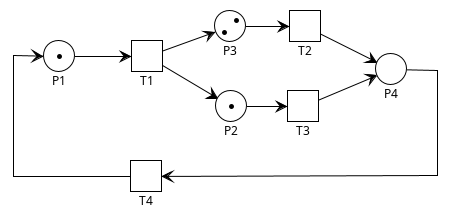
\includegraphics[scale=1.0]{Figures/marco teorico/imag1.png}
	\caption{Red de Petri marcada.}
	\label{fig:rdp2.1_tradicional}
  \end{figure}


\subsection{Estructura de una red de Petri ordinaria} %Referencia aqui 
La estructura de una red de Petri puede definirse como una tupla de 5 elementos (5-tupla)\cite{falko} de la siguiente manera:

\begin{equation}
    N = (P, T, I^- , I^+ , M_0) 
\end{equation}

\noindent Donde:
\begin{itemize}
    \item $ P = \{P_1 , P_2,..., P_n \}$ es un conjunto finito y no vacío que contiene todas las plazas de la red.
    \item $T = \{T_1 , T_2, ... ,T_m \}$ es un conjunto finito y no vacío que contiene todas las transiciones.
    \item $I^{-}$ y $I^+$ son las matrices \textit{pre} y \textit{post} respectivamente, cuya composición se abordará en la próxima sección.
    \item $M_0$ es el marcado inicial de la red. Definido como un vector con un elemento para cada plaza, donde $M_0[i]$ contendrá la cantidad de \textit{tokens} en la plaza \textit{i} para el estado inicial.
\end{itemize}

Siguiendo con el ejemplo propuesto en la sección anterior (figura \ref{fig:rdp2.1_tradicional}), se puede representar la red como $N = \{P, T, I^- , I^+ , M_0 \}$ donde:

\begin{itemize}
    \item $P = \{P_1 , P_2, P_3 , P_4 \}$ 
    \item $T =  \{T_1, T_2, T_3, T_4\}$
    \item $M_0 = [1,1,2,0]$
\end{itemize}

\noindent A continuación se explicará la manera de obtener las matrices $I^-$ e $I^+$.


\subsection{Matriz de incidencia}
Las matrices  $I^-$ e $I^+$ son las funciones de incidencia de entrada y salida de las plazas. Para el caso de la matriz $I^+$ , denominada post, se tiene que cada elemento $post(P_i , T_j)$ contiene el peso asociado al arco que va desde $T_j$ hasta $P_i$ . Este peso indica la cantidad de \textit{tokens} que se generan en la plaza $P_i$ cuando la transición $T_j$ es disparada. \\
Por otro lado, en la matriz $I^-$ , denominada $pre$, cada elemento $pre(P_i , T_j)$ contiene el peso asociado al arco que va desde $P_i$ hasta $T_j$ e indica la cantidad de $tokens$ que se retiran de la plaza $P_i$ cuando se dispara la transición $T_j$.\\

\hfill \break 
Siguiendo con el ejemplo de la figura \ref{fig:rdp2.1_tradicional} , las matrices $I^-$ e $I^+$ asociadas son:

\begin{equation}
    I^+ = 
    \begin{pmatrix}
        0 & 0 & 0 & 1 \\
        1 & 0 & 0 & 0 \\
        1 & 0 & 0 & 0 \\
        0 & 1 & 1 & 0 \\
    \end{pmatrix}
\end{equation}
\begin{equation}
    I^- = 
    \begin{pmatrix}
        1 & 0 & 0 & 0 \\
        0 & 1 & 0 & 0 \\
        0 & 0 & 1 & 0 \\
        0 & 0 & 0 & 1 \\
    \end{pmatrix}
\end{equation}

Las filas de las matrices representan las plazas mientras que las columnas representan las transiciones, lo cual quiere decir que las matrices tendrán tantas filas como plazas tenga la red de Petri, y tantas columnas como transiciones. \\ \par

De esta forma se puede observar como el elemento $I^-[0][0]$ indica la relación de salida entre $P_1$ y $T_1$ . Más precisamente indica que cuando $T_1$ se dispara, solo un $token$ es retirado de $P_1$ (ya que el peso del arco entre $P_1$ y $T_1$ es 1). De igual manera, el elemento $I^+[0][0] = 0$ indica que cuando la misma transición se dispara, no se genera ningún token en $P_1$ (ya que no existe ningún arco que parta de $T_1$ hacia $P_1$). \\ \par

A partir de estas definiciones, se puede obtener la matriz de incidencia de la red. La misma está definida a continuación:

\begin{equation}
    I = I^+ - I^-
\end{equation}

Cabe aclarar que una red de Petri puede reconstruirse completamente a partir de sus matrices $I^+$ e $I^-$ , pero no así si se tiene sólo la matriz de incidencia $I$. Esto quiere decir que puede haber varias redes de Petri distintas con la misma matriz de incidencia, pero solamente una para las matrices $I^+$ e $I^-$ . Sin embargo, cuando una red de Petri no tiene autobucles (presente cuando se tienen dos arcos (con sentidos contrarios) entre una misma plaza y transición), su matriz de incidencia determina completamente su estructura. \\ \par

\textsc{Ejemplo} La matriz de incidencia asociada a la red de Petri de la figura \ref{fig:rdp2.1_tradicional} será entonces:

\begin{equation}
    I = 
    \begin{pmatrix}
        0 & 0 & 0 & 1 \\
        1 & 0 & 0 & 0 \\
        1 & 0 & 0 & 0 \\
        0 & 1 & 1 & 0 \\
    \end{pmatrix}
    -
    \begin{pmatrix}
        1 & 0 & 0 & 0 \\
        0 & 1 & 0 & 0 \\
        0 & 0 & 1 & 0 \\
        0 & 0 & 0 & 1 \\
    \end{pmatrix}
    = 
    \begin{pmatrix}
        -1 & 0 & 0 & 1 \\
        1 & -1 & 0 & 0 \\
        1 & 0 & -1 & 0 \\
        0 & 1 & 1 & -1 \\
    \end{pmatrix}
\end{equation}


%----------------------------------------------------------------------------------------
%	SECTION 2
%----------------------------------------------------------------------------------------
\section[Dinámica de una red de Petri]{Dinámica de una red de Petri} \label{sec:drdp}

Se dice que una transición está sensibilizada cuando el marcado de todas las plazas entrantes a la transición es mayor o igual al peso de los arcos que las unen con dicha transición.\cite{papermico}  \\
Antes de expresar la condición de sensibilizado de manera general, es necesario definir los siguientes conjuntos y funciones:

\begin{itemize}
    \item $\bullet T_j$ es el conjunto compuesto por las plazas entrantes a $T_j$.
    \item $T_j \bullet$  es el conjunto compuesto por las plazas salientes de $T_j$.
    \item $\bullet \bullet P_i$ es el conjunto compuesto por las transiciones entrantes a las plazas que sensibilizan a las transiciones que le \textit{agregan} tokens a $P_i$.
    \item $P_i \bullet \bullet$  es el conjunto compuesto por las transiciones entrantes a las plazas que sensibilizan a las transiciones que le \textit{quitan} tokens a $P_i$.
    \item $m_k(P_i)$ es el marcado de la plaza Pi antes de disparar la transición $T_j$ .
    \item $m_{k+1}(P_i)$ es el marcado de la plaza $P_i$ después de disparar la transición $T_j$.
    \item $w_{ij}$ es el peso del arco $P_i \rightarrow T_j$.
    \item $w_{ji}$ es el peso del arco $T_j \rightarrow P_i$.
\end{itemize}

\noindent Entonces, el sensibilizado de una transición $T_j$ está dado por:

\begin{equation}
    T_j \ est\acute{a} \ sensibilizada \ sii \ \forall \ P_i \ \in \ \bullet T_j \Rightarrow m_k (P_i) > w_{ij}
\end{equation}

Esta definición de sensibilizado es solo válida cuando los arcos que conectan las plazas con $T_j$ son arcos comunes. \\
En la figura \ref{fig:rdp2.2_marcada} se resaltan las transiciones sensibilizadas del ejemplo anterior.

\begin{itemize}
    \item $T_1$, $T_2$, $T_3$ están sensibilizadas, mientras $T_4$ no está sensibilizada (ya que el marcado de $P_4$ es menor al peso del arco $P_4$ \rightarrow $T_4$ ).
\end{itemize}

\begin{figure}[H]
	\centering
	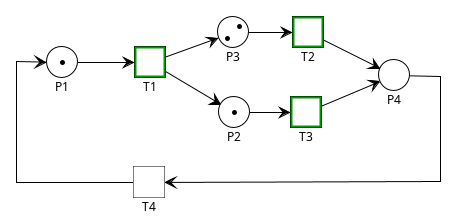
\includegraphics[scale=1.00]{Figures/marco teorico/imag2.png}
	\caption{Transiciones sensibilizadas de la red de Petri.}
	\label{fig:rdp2.2_marcada}
  \end{figure}


\subsection{Disparo de una transición}
Si una transición está sensibilizada, la misma puede dispararse. El disparo de una transición resulta en un nuevo marcado de la red. Más precisamente, al ejecutarse una transición $T_j$ con un marcado $m_k$, los marcados de las plazas pertenecientes a la red se alteran cumpliendo con las siguientes declaraciones:

\begin{equation}
    \sigma (m_k, T_j) = 
    \begin{array}{cc}
         \forall \ P_i \ \in \ \bullet T_j \ \Rightarrow \ m_{k+1}(P_i) = m_k(P_i) - w_{ij}  \\
         \forall \ P_i \ \in \ T_j \bullet \ \Rightarrow \ m_{k+1}(P_i) = m_k(P_i) + w_{ji}  \\
         \forall \ P_i \ \notin \ \bullet T_j \cup T_j \bullet \ \Rightarrow m_{k+1}(P_i) = \ m_k(P_i)
    \end{array}
\end{equation}

\noindent Es decir:
\begin{itemize}
    \item Para todas las plazas entrantes a $T_j$, el nuevo marcado de cada plaza se habrá \textbf{decrementado} tantos $tokens$ como peso tenga el arco $P_i \rightarrow T_j$. 
    \item Para todas las plazas salientes de $T_j$, el nuevo marcado de cada plaza se habrá \textbf{incrementado} tantos $tokens$ como peso tenga el arco $T_j \rightarrow P_i$.
    \item Para el resto de las plazas, el nuevo marcado será exactamente igual al que tenían antes del disparo de $T_j$ .
\end{itemize}

Continuando con el ejemplo anterior, se puede observar en la figura \ref{fig:rdp2.3_disparada} el nuevo marcado de la red luego del disparo de la transición $T_3$:

\begin{itemize}
    \item La única plaza entrante a $T_3(P_3 )$, ha \textbf{decrementado} su marcado en 1 $token$ (ya que el peso del arco $P_3 \rightarrow T_3$ es 1).
    \item La plaza saliente de $T_j(P_4)$ ha \textbf{incrementado} su marcado de acuerdo a los pesos de los arcos correspondientes, en este caso en 1.
    \item Las plazas que no es entrante ni saliente de $T_3(P_3)$ ha mantenido su marcado original.
\end{itemize}

Cabe destacar que como consecuencia del disparo de $T_3$, se ha producido la sensibilización de $T_4$.

\begin{figure}[H]
	\centering
	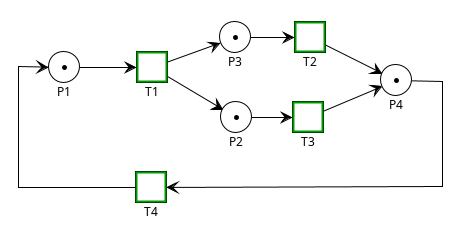
\includegraphics[scale=1.00]{Figures/marco teorico/imag3.png}
	\caption{Nuevo marcado de la red de Petri.}
	\label{fig:rdp2.3_disparada}
  \end{figure}


\subsection{Función de transferencia y ecuación de estado}
Una vez explicada la dinámica del disparo de una transición y la forma de obtener la matriz de incidencia, se detalla una expresión matemática necesaria para obtener el nuevo marcado luego del disparo de una transición. 
La misma se denomina \textbf{función de transferencia} y está definida como el producto de la matriz de incidencia $I$ con un vector $\vec{\delta}$ cuyos componentes son todos ceros, exceptuando el componente asociado a la transición que se quiere disparar, cuyo valor será uno. Entonces, se tendrá:

\begin{equation}
    I \ . \ \vec{\delta }    
\end{equation}

\noindent donde, para el disparo de una transición $T_j$ , se tiene:
\begin{itemize}
    \item $\delta[j] = 1$
    \item $\delta[i] = 0 \ \forall \ i/i \neq j$
\end{itemize}

Por otro lado, es necesario introducir la \textbf{ecuación de estado} de las redes de Petri. Con esta ecuación es posible obtener el siguiente estado del sistema luego del disparo de una transición. Esta es una manera más simple que la metodología gráfica para analizar la evolución de los sistemas. La ecuación de estado en un tiempo $i$, para calcular el nuevo marcado de la red en un tiempo $i+1$ se define como:

\begin{equation}
    M_{i+1} = M_i + I \ . \ \vec{\delta}
    \label{ec:estado}
\end{equation}

\noindent donde $M_{i+1}$ es el marcado luego del disparo de la transición, $M_i$ es el marcado antes del disparo y el segundo término de la ecuación es la función de transferencia.

Siguiendo con el ejemplo hasta ahora analizado se verá cómo calcular el marcado de la red luego del disparo de la transición $T_3$ haciendo uso de la ecuación de estado.

En la figura \ref{fig:rdp2.2_marcada} se observan las transiciones sensibilizadas de la red para el marcado inicial $M_0$.
\\
La ecuación de estado requiere tres elementos:

\begin{enumerate}
    \item El marcado antes del disparo. Éste es:
        \begin{equation}
            M_i = M_0 = 
            \begin{pmatrix}
                1 \\
                1 \\
                2 \\
                0
            \end{pmatrix}
        \end{equation}
        
    \item La matriz de incidencia de la red. La misma fue calculada en la sección 2.1.2 y es la siguiente:
        \begin{equation}
           I = 
            \begin{pmatrix}
                -1 & 0 & 0 & 1 \\
                1 & -1 & 0 & 0 \\
                1 & 0 & -1 & 0 \\
                0 & 1 & 1 & -1 
            \end{pmatrix}
        \end{equation}
        
    \item El vector de disparo $\vec{\delta}$, que tendrá tantos elementos como transiciones haya en la red, cuyos valores serán cero para todas las transiciones excepto para aquella que se desee dispara:
        \begin{equation}
            \vec{\delta} = 
            \begin{pmatrix}
                0 \\
                0 \\
                1 \\
                0
            \end{pmatrix}
        \end{equation}
\end{enumerate}

\noindent con lo cual el nuevo marcado está definido por:
\begin{equation}
    M_{i+1} = 
    \begin{pmatrix}
        1 \\
        1 \\
        2 \\
        0
    \end{pmatrix}
    +
    \begin{pmatrix}
        -1 & 0 & 0 & 1 \\
        1 & -1 & 0 & 0 \\
        1 & 0 & -1 & 0 \\
        0 & 1 & 1 & -1 
    \end{pmatrix}
    .
    \begin{pmatrix}
        0 \\
        0 \\
        1 \\
        0
    \end{pmatrix}
    =
    \begin{pmatrix}
        1 \\
        1 \\
        1 \\
        1
    \end{pmatrix}    
\end{equation}

\noindent resultado que coincide con lo obtenido en la figura \ref{fig:rdp2.3_disparada}. La ecuación de estado representa matemáticamente el comportamiento dinámico del sistema, permitiendo calcular el nuevo estado del mismo luego de la ocurrencia de un evento a través de una simple ecuación.

\subsection{Extensión de la ecuación de estado}
Como se mencionó en la sección anterior, la ecuación \ref{ec:estado} permite calcular el siguiente estado luego del disparo de una transición. Sin embargo, puede que se desee obtener el marcado final luego de una secuencia de disparos. Suponiendo que se parte del estado inicial $M_0$, esto puede representarse como:

\begin{equation}
    M_i = M_0 + I \ . \sum_{j=1}^i u_j
\end{equation}

\noindent donde la sumatoria representa un vector asociado a la secuencia de transiciones que se desea disparar y se denomina vector S. Para ejemplificar, el cálculo de un marcado $M_i$ a partir del marcado inicial y luego del disparo de las transiciones {$T_3$, $T_4$, $T_1$, $T_2$,} está dado por:

\begin{equation}
    M_i = M_0 + I \ . \ \vec{S}
\end{equation}

\noindent donde $\vec{S}$ = \{ 1, 1, 1, 1 \} e $I$ es la matriz de incidencia asociada a la red.

%----------------------------------------------------------------------------------------
%	SECTION 3
%----------------------------------------------------------------------------------------
\section{Propiedades de las redes de Petri} \label{sec:gestionred}
\subsection{Propiedades de limitación}
Dada una red de Petri definida por $PN = \{ P, T, I^-, I^+, M_0 \}$, se dice que una plaza P está k-limitada si existe un número entero k que, para todo marcado posible de la red, se verifica que la cantidad de tokens de la plaza siempre es igual o menor a k. Es decir:


\begin{equation}
    \exists \ k \ \in \ N \ / \ \forall \ M \ \in \ marcados (PN) \Rightarrow M(P) \leq k
\end{equation}

\noindent Por otro lado, se dice que la red está \textbf{k-limitada} si todas las plazas que contiene son \textbf{k-limitadas}. \\ \par

A partir de la definición de limitación surgen varios conceptos, entre los cuales se encuentran los siguientes:
\begin{itemize}
    \item Una red de Petri es \textbf{segura} si todas sus plazas son \textbf{1-limitadas}. Esto significa que nunca puede darse un disparo si la plaza de llegada ya contiene un $token$.
    
    \item Una red de Petri es \textbf{cíclica} si siempre existe la posibilidad de alcanzar el marcado inicial desde cualquier otro marcado alcanzable. Es decir, \break $\forall \ M  \in \ marcados(PN),\ M_0$ es dinámicamente alcanzable desde $M$.
    
    \item Una red de Petri es \textbf{repetitiva} si existe una secuencia de disparos $\sigma$ que contiene todas las transiciones de la red y existe un marcado $M$ que para el cual $M \xrightarrow{\sigma} M$. Es decir, existe una secuencia de disparos que contiene todas las transiciones y que lleva la red del marcado actual al mismo marcado.
    
    \item  Una red de Petri es \textbf{conservativa} si se cumple que $\forall \ M\ \in marcados (PN)$, el número total de $tokens$ en el marcado M es igual al número de tokens en el marcado $M_0$. En otras palabras, la red siempre contiene la misma cantidad de marcas.
    
\end{itemize}

\subsection{Propiedades de vivacidad}
La \textbf{vivacidad} de una transición indica que, en todo instante de la  evolución de la red, su disparo es posible. Este concepto es particularmente relevante ya que determina si la ejecución de la red puede  o no detenerse en un estado determinado. A partir de esto se puede definir la vivacidad de una red de Petri. Esta propiedad indica que una red $N = \{P, T, I^- , I^+ , M_0 \}$ es viva para un marcado si todas sus transiciones lo son.

Por otro lado, la \textbf{cuasi-vivacidad} de una transición expresa la posibilidad de dispararla al menos una vez a partir de un marcado inicial $M_0$. De la misma manera que para el caso de la vivacidad, una red de Petri es cuasi-viva si todas sus transiciones lo son.

Gracias a esta última definición, se puede definir la vivacidad en función de la cuasi-vivacidad de la siguiente manera: una transición es viva si la misma es cuasi-viva en la red para todo marcado alcanzable desde $M_0$. \\ \par

\noindent La vivacidad está directamente asociada con la ausencia de \textbf{deadlock} o interbloqueo. En términos generales, el deadlock es el bloqueo permanente de un conjunto de procesos o hilos de ejecución en un sistema concurrente que compiten por recursos del sistema o bien se comunican entre ellos. En el caso de una red de Petri, esto suele ocurrir cuando dos o más transiciones esperan mutuamente por el disparo de la otra, produciendo el bloqueo permanente de esa porción de la red. 
Una red de Petri viva garantiza la ausencia de interbloqueo sin importar la secuencia de disparos.


\subsection{Alcanzabilidad de una red de Petri}
La \textbf{alcanzabilidad} de una red de Petri es fundamental para el análisis de las propiedades dinámicas de un sistema. A grandes rasgos, permite determinar si el sistema modelado puede alcanzar un determinado estado.


Un marcado $M_i$ es alcanzable desde $M_0$ si existe una secuencia finita de disparos $\sigma$ tal que $M_0 \xrightarrow{\sigma} M_i$.

Los marcados alcanzables por la red pueden ser representados como nodos de un grafo o árbol, donde los arcos indican los disparos necesarios para alcanzar dicho marcado. El algoritmo para determinar el árbol de alcanzabilidad de una red de Petri será explicado con detalle en el desarrollo del proyecto.

Entonces, el grafo de alcanzabilidad $A$ se define como el menor conjunto que cumpla con las expresiones 2.17 y 2.18.

\begin{equation}
    M_0 \ \in \ A
\end{equation}

\noindent Esta condición simplemente aclara que el marcado inicial de la red siempre forma parte del grafo de alcanzabilidad, ya que el mismo no requiere ninguna secuencia de disparos para ser alcanzable.

\begin{equation}
    \forall \ M \ sii \ M \xrightarrow{\sigma} M_i \Rightarrow M_i \ \in \ A
\end{equation}


\noindent Esto significa que para cualquier marcado $M$, si a partir del mismo puede alcanzarse otro marcado $M_i$, entonces $M_i$ forma parte del grafo. \\ \par

\noindent \textsc{Ejemplo} \ Suponiendo una red simple como la de la figura \ref{fig:rdp2.4_estadosposibles}, compuesta por tres plazas y una única transición $T_1$ , se puede afirmar que sólo hay tres estados posibles en la red:

\begin{figure}[H]
	\centering
	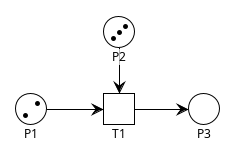
\includegraphics[scale=1.00]{Figures/marco teorico/imag4.png}
	\caption{Red de Petri 3 estados posibles.}
	\label{fig:rdp2.4_estadosposibles}
  \end{figure}
  
\begin{itemize}
    \item El marcado inicial [2, 3, 0]
\end{itemize}

Luego del segundo disparo no existen disparos posibles. Por lo tanto, la red de la figura \ref{fig:rdp2.4_estadosposibles} produce el grafo de alcanzabilidad  mostrado en la figura \ref{fig:rdp2.5_grafo}. \\

\begin{figure}[H]
	\centering
	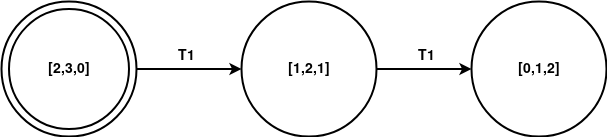
\includegraphics[scale=0.5]{Figures/marco teorico/grafoalcanzabilidad.png}
	\caption{Grafo de alcanzabilidad.}
	\label{fig:rdp2.5_grafo}
  \end{figure}

\subsection{Sifones y Trampas} \label{sec:tysalg2}
Los conceptos de sifón y trampa están directamente relacionados con las propiedades de \textbf{interbloqueo} y \textbf{vivacidad} de una red de Petri.

Un \textbf{sifón} se define como un subconjunto no vacío de plazas S para el cual se cumple que el subconjunto de transiciones entrantes a S está contenido dentro del subconjunto de transiciones salientes de S.
En otras palabras, un grupo de plazas es un sifón si, una vez que un token sale del grupo de dichas plazas, el mismo nunca puede volver a entrar. 
Decimos que un sifón S es \textbf{mínimo} si no contiene otro sifón como un subconjunto. En un sifón mínimo debe existir al menos dos lugares; de lo contrario, la estructura restante no puede considerarse un sifón.
En la figura \ref{fig:rdp2.6-sifontrampa} se puede observar una red que contiene una trampa y un sifón.

\begin{figure}[H]
	\centering
	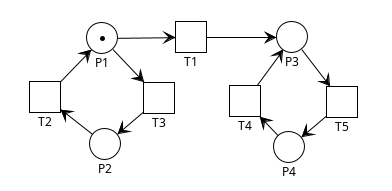
\includegraphics[scale=1.00]{Figures/marco teorico/imag6.png}
	\caption{Sifón y trampa.}
	\label{fig:rdp2.6-sifontrampa}
  \end{figure}
  
Tomando el subconjunto de plazas $S = \{P_1 , P_2 \}$ se deben obtener los siguientes subconjuntos de transiciones:
\begin{itemize}
    \item El subconjunto $\bullet S = \{T_2, T_3 \}$ será aquel compuesto por las transiciones entrantes a las plazas que componen S.
    \item El subconjunto $S \bullet = \{T_2, T_3\} $ será aquel compuesto por las transiciones entrantes a las plazas que componen S.
\end{itemize}

\noindent Por propiedad de los sifones, para que S pueda considerarse como tal debe cumplirse que:
\begin{equation}
    \bullet S \ \subseteq \ S \bullet 
\end{equation}

En este caso, se comprueba que ${T_2 , T_3} \subseteq \ \{T_1 , T_2 , T_3 \}$, quedando demostrado que $\{P_1,P_2\}$ es en efecto un sifón y que, si la transición $T_1$ se dispara, el token removido de $P_1$ nunca volverá a ingresar al subconjunto. \\ \par

Por otro lado, una \textbf{trampa} se define como un subconjunto de plazas G para el cual se cumple que el subconjunto de transiciones salientes de G está contenido dentro del subconjunto de transiciones entrantes a G. Esto quiere decir que un conjunto de plazas constituyen una trampa si una vez que un token entra dicho grupo éste nunca vuelve
a salir.

Siguiendo con el ejemplo de la figura \ref{fig:rdp2.6-sifontrampa}, se analizará el subconjunto de plazas $G = \{P_3 , P_4\}$.  Los subconjuntos de transiciones serán:
\begin{itemize}
    \item El subconjunto $\bullet G = \{T_1 , T_4 , T_5 \}$ será aquél compuesto por las transiciones entrantes a las plazas que componen G.
    \item El subconjunto $G \bullet = \{T_4, T_5 \}$ será aquél compuesto por las transiciones salientes de las plazas que componen G.
\end{itemize}

\noindent Por propiedad de las trampas, para que G pueda considerarse como tal, debe cumplirse que:
\begin{equation}
    G \bullet \ \subseteq \ \bullet G
\end{equation}

Propiedad que es simplemente comprobable ya que ${T_4 , T_5} \subseteq \{T_1 , T_4 , T_5 \}$, demostrando que $\{P_3 , P_4\}$ es una trampa.


\subsection{Invariantes de plazas y transiciones}
Las invariantes de una red son propiedades independientes tanto del marcado inicial como de la secuencia de disparos, y pueden asociarse a ciertos subconjuntos de plazas o de transiciones; con lo cual surgen dos conceptos:

\subsubsection{P-invariantes}
Una \textbf{invariante de plazas} o \textbf{P–invariante} es un conjunto de plazas cuya suma de tokens no se modifica con una secuencia de disparos arbitraria. 
Esto se puede observar en el ejemplo de la figura \ref{fig:rdp2.7_p-invariante}:

\begin{figure}[H]
	\centering
	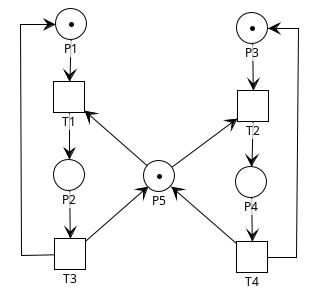
\includegraphics[scale=0.8]{Figures/marco teorico/imag7.png}
	\caption{P-invariantes de la red de Petri.}
	\label{fig:rdp2.7_p-invariante}
  \end{figure}
 
 \noindent Tras el análisis de la red , se obtienen las siguientes invariantes de plazas:
 
 \begin{equation}
    \begin{array}{cc}
        m(P_1) + m(P_2) = 1  \\
        m(P_3) + m(P_4) = 1   \\
        m(P_2) + m(P_4) + m(P_5) = 1 
    \end{array}
 \end{equation}

El primer ítem expresa que la sumatoria de tokens en las plazas $P_1$ y $P_2$ siempre será igual a uno, afirmación completamente observable al mirar la red de la figura \ref{fig:rdp2.7_p-invariante}. Estas declaraciones implican la siguiente consecuencia:

\begin{equation}
    I . x = 0
\end{equation}

\noindent donde $I$ es la matriz de incidencia y $x$ es un vector característico de un subconjunto $Q$ de las plazas que forman parte de la invariante (un uno en una posición indica que esa plaza es parte de la invariante y un cero indica lo contrario). A partir de esto surge la siguiente fórmula:

\begin{equation}
    \sum_{P \in \bullet t \cap Q} W(p,t) = \sum_{P \in t \bullet \cap Q} W(t,p)
\end{equation}

\noindent la cual puede ser expresada en función de un vector t de la siguiente manera:

\begin{equation}
    \sum_{P \in \bullet t \cap Q} t(p) = \sum_{P \in t \bullet \cap Q} t(p)
\end{equation}

\noindent Esto quiere decir que:

\begin{equation}
    \sum_{P \in (t \bullet \cup \bullet t) \cap Q} t(p) = 0 \ \ y \  \sum_{P \in Q} t(p) = 0
\end{equation}

Si reemplazamos Q por los vectores característicos $I_q$ , estas dos igualdades pueden escribirse como:

\begin{equation}
    \sum_{P \in Q} t(p) I_q(p) = 0 \ \ y \  \sum_{p \in P} t(p)I(p) = 0
\end{equation}

\noindent Lo cual es simplemente la definición del producto escalar entre dos vectores:

\begin{equation}
    t.I_q = 0
\end{equation}

\noindent Como los disparos son arbitrarios, podemos establecer la siguiente relación:
\begin{equation}
    t_j I_q; \forall \ t_j \ \in \ T \Longleftrightarrow \ I^T I_q = 0
\end{equation}

\noindent donde $I^T$ es la matriz de incidencia transpuesta.


\subsubsection{T-invariantes}
Un \textbf{invariante de transición} ó \textbf{T-invariante} es el conjunto de transiciones que deben dispararse para que la red de Petri retorne a su estado inicial.

Como se mencionó en el apartado anterior, para el cálculo de las P-invariantes se hace uso de la ecuación $I . x = 0$, siendo $I$ la matriz de incidencia y $x$ un vector característico constituido por las plazas que forman parte de la invariante. En este caso, para el cálculo de los vectores que constituyen las T-invariantes, la ecuación asociada será similar a las P-invariantes, a diferencia que se hace uso de  $I^T$ en vez de $I$:

\begin{equation}
    I^T . x = 0
\end{equation}

Aquí, a diferencia de las P-invariantes, el vector x está constituido por el conjunto de transiciones que deben dispararse para que la red retorne al estado inicial. Un "1" en una posición indica que esa transición es parte de la invariante y un "0" indica lo contrario.

Tomando la figura \ref{fig:rdp2.7_p-invariante} como ejemplo y se obtienen las siguientes invariantes de transiciones:

\begin{equation}
    T-invariantes = 
    \begin{pmatrix}
         T0 & T1 & T2 & T3  \\
         0 & 1 & 0 & 1  \\
         1 & 0 & 1 & 0  
    \end{pmatrix}
\end{equation}

Ambos vectores cumplen la condición planteada ($I^T .\ x = 0$) y si se observa la imagen en cuestión, se puede apreciar que la red retorna a su estado inicial si las transiciones especificadas en los vectores se disparan.


%-----------------------------------------------------
% Monitores (SECTION 4)
%-----------------------------------------------------
\section{Concurrencia y sincronización} \label{sec:monitor}
En los sistemas de computación actuales conviven múltiples procesos que cooperan para lograr determinados objetivos y compiten por recursos del sistema, entre ellos el procesador, la memoria RAM, los puertos de entrada/salida, etc.\\
Dado que generalmente el numero de procesos de un sistema supera ampliamente el numero de recursos, se deben establecer formas de comunicación y sincronización entre ellos que hagan que el sistema funcione correctamente. 

\par En ésta sección se definirá cuando dos programa son concurrentes y/o paralelos y las condiciones que deben cumplirse para que dos secciones de código fuente puedan ser ejecutadas de manera concurrente. Luego, se verá que la ejecución concurrente de procesos trae aparejados ciertos problemas como el interbloqueo y la inanición.\\
Por esta razón deben ejecutarse ciertos mecanismos de control para garantizar la correcta ejecución de los programas, entre ellos, los semáforos y monitores.\\
El objetivo de esta sección es que el lector adquiera una idea general sobre la programación concurrente y sobre los problemas inherentes a la misma.


\subsection{Concurrencia y paralelismo}
Dos procesos serán concurrentes cuando la primera instrucción de uno de ellos se ejecuta después de la primera instrucción de otro proceso y antes de la última.
No es necesario que estos se ejecuten al mismo tiempo, basta con el hecho de que se intercalen sus instrucciones. En caso de ejecutarse al mismo tiempo se dice que hay programación paralela.
La programación concurrente es un paralelismo potencial, dependiente del hardware que lo soporte  \cite{mendez}.

\subsubsection{Problemas inherentes a la programación concurrente}
La intercalación de instrucciones de diferentes procesos, debe ser bien manejada y controlada dado que puede producir mal funcionamiento del sistema. Los problemas inherentes a la concurrencia son:
\begin{itemize}
    \item \textbf{Exclusión mutua}: Se debe garantizar que si un proceso adquiere el recurso los demás deberán esperar hasta que sea liberado.

    \item \textbf{Condición de sincronización}: Hay situaciones en las que un proceso debe esperar que ocurra algún determinado evento para poder continuar. Por ello se debe garantizar que si el evento \textbf{no} ocurrió, el proceso \textbf{no} continúe. 
    
    \item \textbf{Interbloqueo}: Esta situación se produce cuando todos los procesos están esperando un evento que nunca ocurrirá. Se debe garantizar que estas situaciones no ocurran.
    
    \item \textbf{Inanición}: En este caso, el sistema en su conjunto hace progresos, pero existe un grupo de procesos que nunca progresaran pues no se les otorga tiempo de procesador para hacerlo.
\end{itemize}

\subsubsection{Exclusión mutua}
La exclusión mutua implica que dos o más procesos intentan acceder a un único recurso compartido entre ellos pero solo uno puede acceder a cada instante.
Cuando se da un caso de estas características, se desea que todo lo que necesite hacer unos de los procesos sobre el recurso se realice de manera indivisible y luego lo deje disponible para que otro proceso ejecute sus instrucciones sobre el recurso.
\par A la porción de código que se desea que se ejecute de manera indivisible o atómica se le llama \textbf{sección crítica}. Se debe lograr que todas las instrucciones dentro de la sección crítica se ejecuten en exclusión mutua lo que implica que el hecho de que cuando uno de los procesos este ejecutando esa porción de código el resto no podrá hacerlo. \\
\\
\textbf{Solo uno de los procesos podrá estar en la sección crítica en un instante dado.}

\begin{figure}[H]
	\centering
	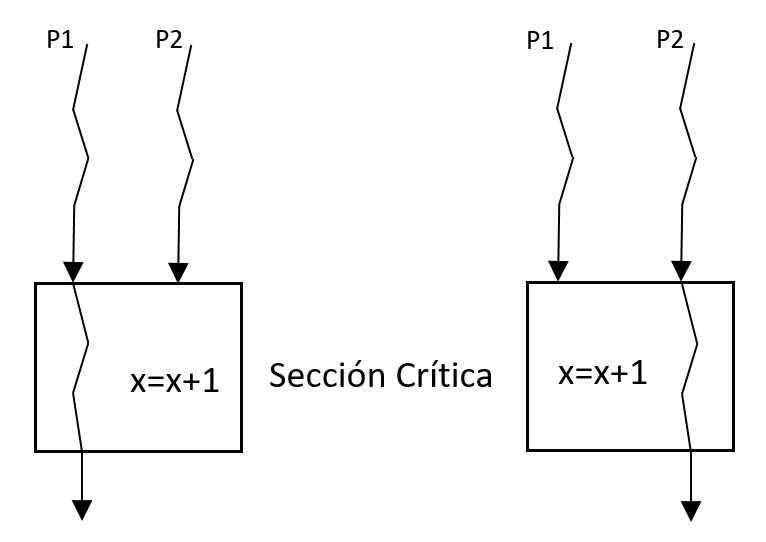
\includegraphics[scale=0.5]{Figures/marco teorico/seccion.jpg}
	\caption{Sección crítica.}
	\label{fig:seccioncritica}
  \end{figure}
  
En la figura \ref{fig:seccioncritica} se observa como dos procesos $P1$ y $P2$ intentan ejecutar una porción de código de una sección crítica. La imagen de la izquierda (a) muestra que el proceso $P1$ consigue ingresar a ejecutar la sección crítica. La imagen de la derecha (b) muestra que el proceso $P2$ puede ingresar solo cuando el proceso $P1$ ya no esta en la misma.

\noindent La exclusión mutua se puede representar de la siguiente manera.
\begin{figure}[H]
	\centering
	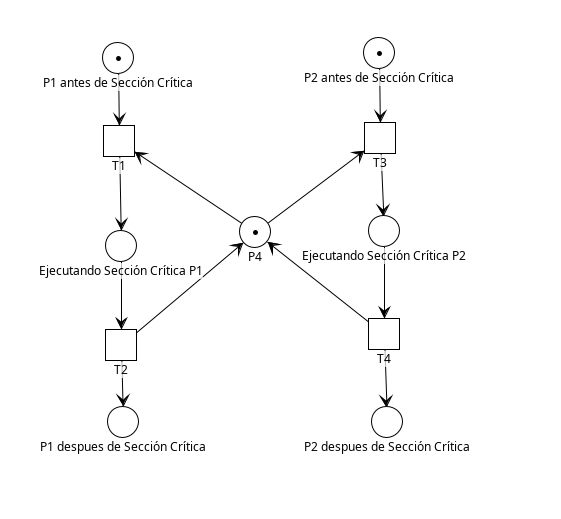
\includegraphics[scale=0.7]{Figures/marco teorico/mutex.png}
	\caption{Sección crítica.}
	\label{fig:exmutuardp}
  \end{figure}

En la figura \ref{fig:exmutuardp} la plaza \textit{MUTEX} esta limitada a un único token y el análisis de invariantes de plazas demuestra formalmente la propiedad de exclusión mutua entre los procesos $P1$ y $P2$. 

\begin{equation}
    m(EjecutandoSCP1) + m(MUTEX) + m(EjecutandoSCP2) = 1
\end{equation}

\subsection{Interbloqueo} \label{sec:Interbloqueo}
En un sistema donde los procesos compiten por limitados recursos, pueden producirse demandas contradictorias de los mismos. Por ejemplo, si existen dos procesos, \textit{A} y \textit{B}, y dos recursos \textit{R1} y \textit{R2}, y ambos procesos necesitan los dos recursos para proseguir, si el proceso \textit{A} toma el recurso \textit{R1} y el \textit{B} el recurso \textit{R2}, ambos procesos se bloquearan a la espera del otro recurso, pero ninguno liberará el recurso que posee hasta no conseguir los dos. A esta situación se la conoce como interbloqueo \cite{stallings}. 

\subsubsection{Condiciones para producir interbloqueo: }
\noindent Deben presentarse tres condiciones de gestión para que sea posible un interbloqueo:
\begin{enumerate}
    \item \textit{Exclusión mutua}: sólo un proceso puede utilizar un recurso en cada momento. Ningún proceso puede acceder a un recurso que se ha asignado a otro proceso.
    
    \item \textit{Retención y espera}: un proceso puede mantener los recursos asignados mientras espera la asignación de otros recursos.
    
    \item \textit{No apropiación}: ningún proceso podrá ser forzado a abandonar un recurso que retiene.
    
    \item \textit{Espera circular}: existe una cadena cerrada de procesos donde cada proceso retiene un recurso que necesita un proceso que le sigue en la cadena.
\end{enumerate}

Las tres primeras condiciones son necesarias pero no suficientes para que exista interbloqueo.
La cuarta es una consecuencia potencial de las tres primeras y, en caso de darse, generará una \textbf{espera circular irresoluble}. Esta es de hecho la definición de interbloqueo.

\subsection{Sincronización}
Para solucionar los problemas inherentes a la programación concurrente, se utiliza lo que se llama \textit{sincronización entre los procesos} . \\
Se habla de sincronización , en general, cuando determinados fenómenos ocurren o deben ocurrir en un determinado orden o a la vez.
\par Para la computación, la sincronización es representada por las señales que se envían los procesos para colaborar entre ellos o para indicar el estado de recursos compartidos, para indicar que un evento o acción ocurrió o no y determinar la continuidad o no de un proceso, etcétera.
\par La condición de sincronización puede definirse como la propiedad requerida para que un proceso no realice ninguna acción o evento hasta que otro proceso realice una determinada acción o evento.


\subsubsection{Semáforos}
Los semáforos son un sistema de señales simples utilizadas por los procesos para comunicarse entre ellos y lograr la sincronización requerida.
Estos tienen una variable de sincronización, del tipo entero no negativo, que indica la cantidad de recursos disponibles. Sobre esta se realizan dos tipos de operaciones:

\begin{itemize}
    \item \textit{wait}: decrementa el valor del semáforo solo si este es mayor que cero. Este proceso indica que se utiliza uno de los recursos que controla el semáforo. Si el valor del semáforo al momento de ejecutar la operación \textit{wait} es cero, indica que no hay recursos disponibles y el proceso deben bloquearse hasta que se libere alguno.
    \item \textit{signal}: es la acción de liberar un recurso que estaba siendo utilizado. En caso de haber algún proceso bloqueado en el semáforo se lo despierta para que utilice el recurso. De no existir algún proceso, se incrementa el valor del semáforo.
\end{itemize}

Los semáforos son primitivas con las cuales es difícil expresar una solución a grandes problemas de concurrencia, ya que tienen algunas debilidades:
\begin{itemize}
    \item La omisión de una de las primitivas puede corromper el funcionamiento de un sistema concurrente.
    \item El control de concurrencia es responsabilidad del programador.
    \item Las primitivas de control se encuentran esparcidas por todo el código, lo que hace muy difícil la corrección de errores y el mantenimiento del mismo.
\end{itemize}

Debido a estas razones existe otro mecanismo de software para el control de concurrencia denominado \textbf{monitor}.

\subsubsection{Monitores}

Como se dijo, los semáforos, generalmente se encuentran dispersos en el código, lo que lo hace más confuso y muchas veces es difícil notar cual es el recurso compartido y determinar si está correctamente sincronizado. Por ello, se necesita un sistema que sea igual de versátil que los semáforos pero que permita efectuar un control más estructurado de la exclusión mutua. Una herramienta con estas características fue propuesta por \textit{C.A.R Hoare} en 1975 y es conocida como \textbf{\textit{monitor}}.\\
Un \textbf{monitor} es un mecanismo de abstracción de datos, lo que permite representar de forma abstracta un recurso compartido mediante variables que indican su estado. El acceso a esas variables solo es posible a través de un conjunto de funciones/métodos que el monitor exporta al exterior.\\

Un monitor se compone de los siguientes elementos:
\begin{itemize}
    \item Un \textit{conjunto de variables} locales que pueden denominarse permanentes. Se utilizan para almacenar el estado interno del recurso que representa el monitor. Se denominan permanentes ya que permanecen sin modificarse entre dos llamadas consecutivas al monitor y solo pueden ser accedidas dentro del mismo.
    
    \item Un \textit{código de inicialización} que se ejecuta antes que la primera instrucción ejecutable del programa y su fin es inicializar las variables permanentes. 

    \item Un \textit{conjunto de procedimientos internos} que manipulan las variables permanentes.
    
    \item Una \textit{declaración de los procedimientos} que son \textit{exportados} y pueden ser accedidos por los procesos activos externos.
\end{itemize}

\paragraph{Exclusión mutua en monitores}
\hfill
\par El control de la exclusión mutua en un monitor se basa en la existencia de una cola asociada al mismo que se denominara \textit{cola del monitor}. La gestión de esta cola se realiza de la siguiente manera:

\begin{enumerate}
    \item Cuando un proceso activo está dentro del monitor (ejecutando alguno de los procedimientos del mismo) y aparece otro proceso activo que intenta ejecutar otro (o el mismo) procedimiento, el código de acceso al monitor bloquea el proceso que realiza la llamada y lo inserta en la cola del monitor (con política FIFO). Así, se impide que dos procesos estén al mismo tiempo dentro del monitor.

    \item Cuando un proceso activo abandona el monitor, este ultimo selecciona el proceso que esta al frente de la cola del monitor y lo desbloquea para que comience a ejecutar las operaciones que le solicitó al monitor. Si la cola estaba vacía, el monitor queda libre y cualquier proceso activo que llame alguno de sus procedimientos entrará al monitor.
\end{enumerate}

Esto asegura que las variables compartidas nunca son accedidas concurrentemente. Una cuestión importante es que la responsabilidad de bloquear un proceso es del monitor y no del proceso.
Al comparar este sistema con un semáforo se ve que en el caso de los semáforos son los propios procesos activos los que manejan las políticas de acceso a variables compartidas.

\paragraph{Condición de sincronización en monitores}
\hfill
\par El procedimiento anterior sólo controla la exclusión mutua, es decir, pueden haber casos donde un proceso activo tenga acceso al monitor (ha obtenido la exclusión mutua al mismo) pero no puede seguir su ejecución debido a alguna razón, tal como un \textit{buffer} lleno que no puede ser escrito. En estos casos, es necesario bloquear ese proceso y permitir que otro ingrese al monitor. Para realizar esto surgen nuevos componentes que deben formar parte del monitor:

\begin{itemize}
    \item Variables de condición
    \begin{itemize}
        \item Las mismas son declaradas en el monitor. 
        \item Deben ser privadas. 
        \item Tienen una cola \textit{FIFO} asociada.
    \end{itemize}
    \item Operaciones sobre las variables de condición
    \begin{itemize}
        \item \textit{Delay}
        \item \textit{Resume}
        \item \textit{Empty}
    \end{itemize}
\end{itemize}

La operación delay se realiza sobre una variable de condición. Si se supone la existencia de una variable C, al realizar \textit{delay(C)}, el proceso que la ejecutó libera el mutex del monitor, se bloquea y se envía al final de la cola asociada a la condición C. A diferencia de la operación wait que se utiliza en los semáforos, delay bloquea al proceso incondicionalmente.\\

\par La operación resume, cuando se realiza sobre una variable C, libera al primer proceso que ejecutó \textit{delay(C)}. Si la cola está vacía, resume es una operación nula. Por otra parte, la función empty simplemente devuelve un valor boolean true si una cola se encuentra vacía o false en caso contrario.\\

Con lo dicho hasta este punto, se podría decir que si un proceso que se está ejecutando dentro del monitor ejecuta una operación \textit{resume(C)}, se desbloqueará un proceso de esa cola que continuará con su ejecución dentro del monitor también. Esto lleva a una situación con dos procesos dentro del monitor, lo que violaría la exclusión mutua. Para evitar esto, el proceso que ejecuta el \textit{resume} cederá la exclusión mutua al recien desbloqueado. Y espera en una cola diferente llamada \textbf{cola de cortesía} hasta que el proceso recién desbloqueado por el \textit{resume(C)} termine su ejecución teniendo preferencia por sobre los procesos esperando en otras colas.


\begin{figure}[H]
	\centering
	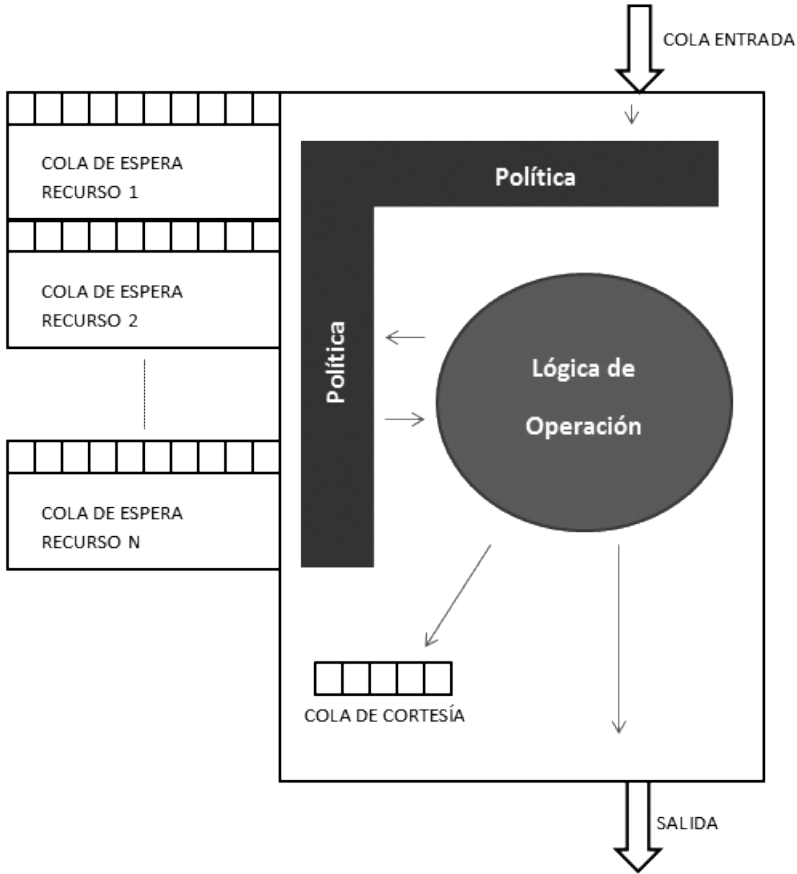
\includegraphics[scale=0.5]{Figures/marco teorico/monitor.png}
	\caption[Monitor.]{Monitor \footnotemark.}
	\label{fig:monitor}
\end{figure} \footnotetext{Figura adaptada del Proyecto Integrador \textit{Desarrollo de IP cores con procesamiento de Redes de Petri Temporales para sistemas multicore en FPGA} \cite{papermico, tesisnonino}.}  
  

\subsubsection{Implementación de monitores con redes de Petri}
Es posible ver a un monitor formado por dos secciones: primero, la referida a la política de colas que se debe ejecutar para lograr que sólo un proceso esté en el monitor, que se bloqueen los procesos que no tienen los recursos y que se desbloqueen los que obtuvieron los recursos, y segundo, la lógica con que se administran los recursos.\\
En la figura \ref{fig:monitor} se puede observar que existe una cola de entrada, para los procesos que aún no ingresaron al monitor y desean hacerlo, una serie de colas, una por cada recurso (cada condición de sincronización) y una cola de cortesía para que  proceso dentro del monitor pueda, de manera segura, ceder la exclusión mutua al cambiar el estado de un recurso.\\

\par \textbf{\textit{Una red de Petri puede realizar el trabajo de la lógica del monitor}}, es decir, la administración y sincronización de recursos disponibles; esto es cuando el vector de estado que resultó del disparo no tiene componentes negativas es porque los recursos están disponibles, el disparo de la transición solicitada conduce a un nuevo estado valido. De no ser así, en caso de existir algún valor negativo en el nuevo vector de estado, se llegó a un estado no válido que indica que el recurso no está disponible. Además el vector de estado indica si el disparo ha devuelto o tomado recursos. Si la cantidad de tokens para un recurso dado disminuye, significa que se han tomado recursos, en caso contrario, que se han devuelto recursos \cite{papermico, tesisnonino}.

\begin{figure}[H]
	\centering
	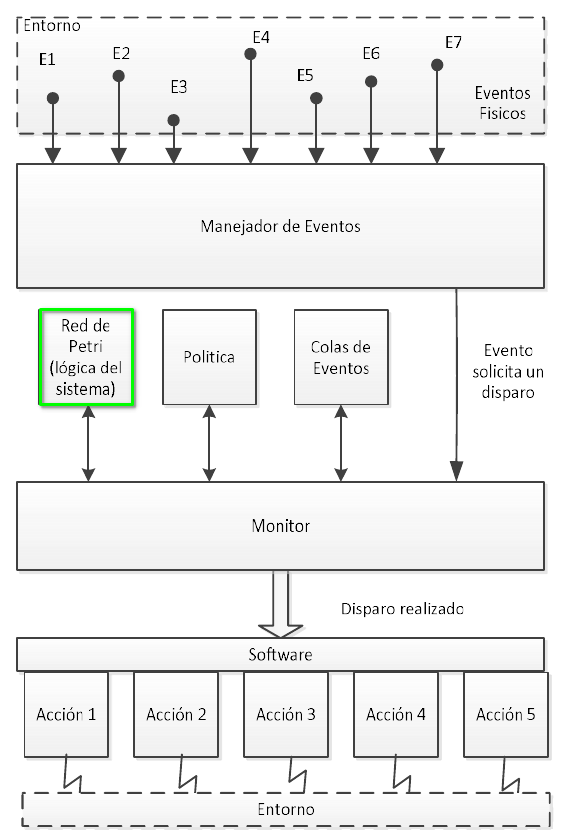
\includegraphics[scale=0.5]{Figures/marco teorico/monitormico.png}
	\caption[Monitor.]{Monitor \footnotemark.}
	\label{fig:monitormico}
\end{figure} \footnotetext{Figura adaptada del paper publicado por \textit{Micolini, Orlando \& Ventre, Luis \& Cebollada, Marcelo \& Eschoyez, Maximiliano} \cite{papermico}}

Por lo tanto, el monitor integra la red de Petri (lógica), la política y las acciones, conformando un sistema heterogéneo. La importancia de la metodología aquí planteada radica en desacoplar la lógica de la política y las acciones, con el fin de obtener un sistema resultante modular, simple, mantenible y verificable. 

En la figura \ref{fig:monitormico} se expone la arquitectura modular de un sistema reactivo y guiado por eventos. Para el interés de este proyecto sólo se investigó sobre la lógica del sistema y específicamente sobre como desbloquear las redes de Petri (del tipo S³PR) que la representa. 


%----------------------------------------------------------------------------------------
%	SECTION 5
%----------------------------------------------------------------------------------------
\section[S³PR]{S³PR}
Definimos la clase de los procesos secuenciales simples (S²P); luego, lo extendemos para modelar el uso de recursos (la clase de S²PR) y, finalmente, definimos la clase de sistemas de procesos secuenciales simples con recursos (S³PR) por la composición neta de S²PR a través de un conjunto de lugares comunes \cite{libro2}.

\subsection{Definición de S²P}
Un sistema de proceso secuencial simple (S²P) es una red de petri $N = (P \cup \{P^0\}, T, F)$ donde:
\begin{enumerate}
    \item $P \neq \emptyset,\ p^0 \notin P$ ($p^0$ llamada plaza idle);
    \item N es una máquina de estado fuertemente conectada
    \item Cada circuito de N contiene la plaza $p^0$.
\end{enumerate}

\noindent La tercera condición impone una propiedad de "terminación" \ a los procesos de trabajo que estamos considerando: si un proceso evoluciona, terminará.

\begin{figure} [H]
    \centering
    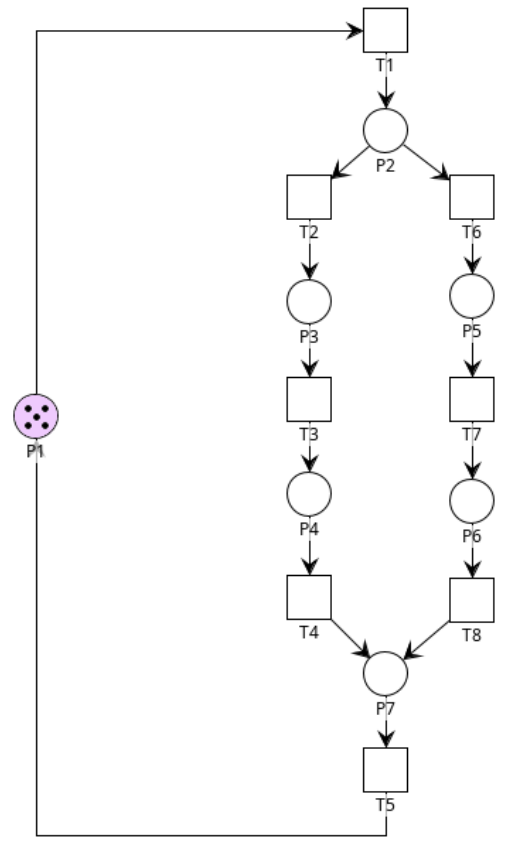
\includegraphics[scale=0.4]{Figures/marco teorico/s2p_chica.png}
    \caption[Red de Petri S²P.]{Red de Petri S²P \footnotemark.}
    \label{fig:rdp_s2p}
\end{figure}  \footnotetext{Figura adaptada del libro \textit{Deadlock Resolution in Automated Manufacturing Systems} \cite{libro2} .}

\noindent En la figura \ref{fig:rdp_s2p} se puede observar la plaza idle ($P_1$) destacada en lila. \\

\par Definimos ahora un proceso secuencial simple con recursos (S²PR), como un S²P que necesita el uso de un recurso único en cada estado que no sea el estado idle. Debido a que las interacciones con el resto de los procesos en el sistema se realizarán compartiendo el conjunto de recursos, es natural suponer que en el estado idle no hay interacción con el resto del sistema y, por lo tanto, no se utiliza ningún recurso en este estado.

\subsection{Definición de S²PR}
Un sistema de proceso secuencial simple con recursos (S²PR) es una red de Petri 
$N = \langle P \cup \{p^0\} \cup P_R, T, F \rangle $ tal que:
\begin{enumerate}
    \item La subred generada por $X = P \cup \{p^0\} \cup T$ es una S²P.
    \item $P_R \neq \emptyset$ y $(P \cup \{p^0\}) \cap P_R = \emptyset$
    \item $\forall p \in P.\ \forall \ t \in \bullet p.\ \forall \ t' \in p \bullet. \ \bullet t \cap P_R = \ t' \bullet \cap P_R = \{r_p\}$
    \item Las dos siguientes declaraciones son verificadas:
    \begin{enumerate}[a)]
        \item $\forall \ r \in \ P_R. \ \bullet \bullet r \cap P = r \bullet \bullet \cap P \neq \emptyset$
        \item $\forall \ r \in \ P_R. \ \bullet r \cap r \bullet = \emptyset$
    \end{enumerate}
    \item $\bullet \bullet (p^0) \cap P_R = (p^0) \bullet \bullet \cap P_R = \emptyset$
\end{enumerate}

\noindent $P_R$: conjunto de plazas de recursos. \\
$P$: conjunto de plazas de estado.

\begin{figure} [H]
	\centering
	\subfloat [] {
	    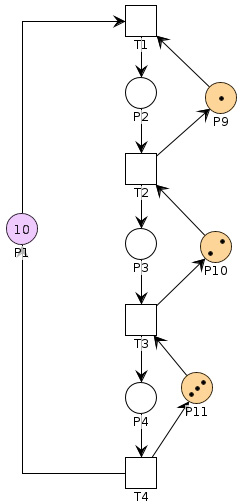
\includegraphics[scale=0.65]{Figures/marco teorico/imag8.jpg}
    	\label{fig:rdp_a}
    }
    \subfloat [] {
        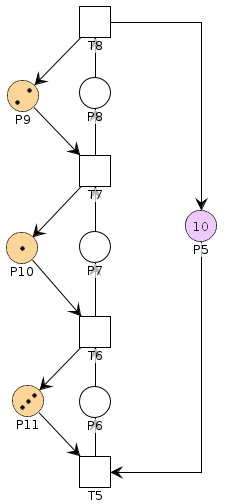
\includegraphics[scale=0.65]{Figures/marco teorico/imag9.jpg}
    	\label{fig:rdp_b}
    } 
   \caption[Redes de Petri S²PR.]{Redes de Petri S²PR. (A) RdP (N1,M1) - (B) RdP (N2,M2) \footnotemark. } 
\end{figure} \footnotetext{Figura adaptada del libro \textit{Deadlock Resolution in Automated Manufacturing Systems} \cite{libro2} .}

\noindent Esto se puede ver representado en las figuras \ref{fig:rdp_a} y \ref{fig:rdp_b}. Las plazas idles ($P_1, P_5$) destacadas en lila, mientras que las plazas recursos ($P_9, P_{10}, P_{11}$) destacadas en naranja.\\


\par Para una plaza de estado dado $p \in P$, la plaza $r \in P_R$ dado por la condición 3 en la definición modela el recurso utilizado en este estado. 
Para un $r \in P_R$, denotaremos $H(r) = (\bullet \bullet r) \cap P$ conjunto de plazas complemento de r (estados que usan r). La condición 4 en la definición anterior impone que dos estados adyacentes de un proceso de trabajo (WP) (ambos diferentes del estado inactivo) no pueden usar el mismo recurso. Esto no es una restricción, ya que desde la perspectiva de la vivacidad, dos estados adyacentes que usan el mismo recurso puede colapsar en un estado único, preservando las propiedades de comportamiento de la red. 

Nótese que $\bullet r$ representa las transiciones entrantes a las plazas r. \\
$\bullet \bullet r = \sideset{}{_{t \in \bullet r}} \bigcup \bullet t$ es el conjunto de plazas de entrada de todas las transiciones de entrada de la plaza r. De manera similar,  $r \bullet \bullet = \sideset{}{_{t \in r \bullet}} \bigcup \bullet t$ representa el conjunto de todas las plazas de salida de todas las transiciones de salida de la plaza r. Por ejemplo, en la figura \ref{fig:s3pr}: $\bullet p9 = \{t_2,t_8\}$ y $\bullet \bullet p_9 =  \bullet t_2 \cup  \bullet t_8 = \{p_2, p_{10}, p_8 \}$.  $p_9 \bullet = \{ t_1, t_7 \}$ y $p_9 \bullet \bullet = t_1 \bullet \cup \ t_7 \bullet = \{ p_2, p_{10}, p_8 \}$. Claramente  $\bullet \bullet p_9 = p_9 \bullet \bullet$

Sea $N = \langle P \cup \{p^0\} \cup P_R, T, F \rangle $ una S²PR. Un marcado inicial $m_0$ es llamado un marcado inicial aceptable para N sii:
\bigskip

\begin{enumerate}
    \centering
    \item $m_0 (p^0) \geq 1$
    \item $m_0 (p) = 0, \ \forall \ p \in \ P$
    \item $m_0 (r) \geq 1, \ \forall \ r \in \ P_R$
\end{enumerate}
\bigskip

Observe que una marca aceptable asigna al menos un token en la plaza idle (entonces, suponemos que, inicialmente, cada marca -token- de cada proceso está inactiva) y al menos un token en cada recurso, es decir, hay al menos una marca de cada recurso en el sistema. Está claro que si existe un recurso para el que no hay marca, el sistema no está bien definido, porque puede tener alguna secuencia de producción que no se puede llevar a cabo. 
\bigskip

\subsection{Definición de S³PR}
Entonces se puede concluir que un sistema de proceso secuencial simple con recursos 
$S^3PR = \{N = \sideset{}{_{n=1}^{k}} \bigcirc = N_i = (P \cup P^0 \cup P_R, T, F)\}$
se define como la unión de un conjunto de redes, de tipo $S^2PR= \{ N_i = (P_i \cup {pi^0} \cup P_{Ri}, T_i, F_i) \}$. Como se puede observar en la figura \ref{fig:s3pr}. \\

\begin{figure} [H]
    \centering
    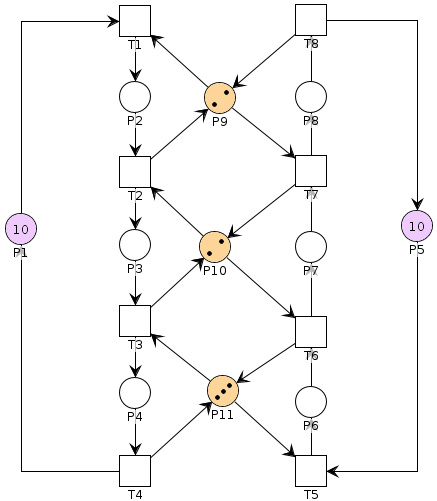
\includegraphics[scale=0.8]{Figures/marco teorico/imag10.jpg}
    \caption[Composición de una red de Petri S³PR.]{Composición de una red de Petri S³PR.\footnotemark}
    \label{fig:s3pr}
\end{figure}  \footnotetext{Figura adaptada del libro \textit{Deadlock Resolution in Automated Manufacturing Systems} \cite{libro2} .}

\newline
Sean $(N_1,M_1)$ y $(N_2,M_2)$ dos redes de Petri con $N_1=(P_1, T_1, F_1, W_1)$ y $N_2 =  (P_2, T_2$, $F_2, W_2)$, donde $P_1 \cap P_2 = P_c \neq \emptyset$  y $T_1 \cap T_2 = \emptyset$. $(N,M)$ con $N = (P, T, F, W)$ es la red resultante de la unión entre $(N_1,M_1)$ y $(N_2,M_2)$ a través de compartir el conjunto de plazas $P_c \ sii (1) P = P_1 \cup P_2$ ,  $T = T_1 \cup T_2$, $F = F_1 \cup F_2$, y $W(x,y) = W_i(x,y)$ si  $(x,y) \in F_i$, $i=1,2$; y (2) $ \forall p \in P_1 \setminus P_c$ , $M(p)=M_1(p)$ , $\forall p \in P_2 \setminus P_c$ , $M(p)=M_2(p)$ y $\forall p \in P_c$ , $M(p)=max\{M_1(p), M_2(p)\}$. \\


Por ejemplo: dos redes $(N_1, M_1)$ y $(N_2, M_2)$ se muestran en la figura \ref{fig:rdp_a} y figura \ref{fig:rdp_b}, respectivamente, donde $P_1= \{p_1-p_4, p_9-p_11\}$, $T_1={t_1-t_4}$, $P_2={p_5-p_{11}}$ y $T_2={t_2-t_8}$. Donde $P_1 \cap P_2 = \{p_9,p_{10},p_{11}\}$ y $T_1 \cap T_2 = \emptyset$. En la figura \ref{fig:s3pr} se observa la red resultante de la composición de $(N_1, M_1)$ y $(N_2, M_2)$ es denotado como $(N,M)$ donde $P = P_1 \cup P_2 = \{p_1-p_{11}\}$, $T = T_1 \cup T_2 = \{t_1-t_8\}$, $M(p_1) = M_1(p_1) = 10$, $M(p_2) = M_1(p_2) = 0$, $M(p_3) = M_1(p_3) = 0$, $M(p_4) = M_1(p_4) = 0$, $M(p_5) = M_2(p_5) = 10$, $M(p_6) = M_2(p_6) = 0$, $M(p_7) = M_2(p_7) = 0$, $M(p_8) = M_2(p_8) = 0$, $M(p_9) = max\{M_1(p_9),M_2(p_9)\} = 2$, $M(p_{10}) = max\{M_1(p_{10})$, $M_2(p_{10})\} = 2$, $M(p_11) = max\{M_1(p_{11}), M_2(p_{11})\} = 3$.



 % Chapter Template 
% cSpell: words Mininet prototipado parencite enrutamiento includegraphics veth  mininetonf cellcolor Nicira vswitchd interconectar multicapa datapath ovsflow resizebox flowtable netlink OVSDB dpctl ofctl vsctl rowcolor mininetovs
 
\chapter{Análisis de las tecnologías} % Main chapter title

\label{Chapter3} % Change X to a consecutive number; for referencing this chapter elsewhere, use \ref{ChapterX}

Teniendo en cuenta los conceptos revisados en el capítulo anterior, en este se estudiarán las herramientas que permitirán la realización del proyecto. 

En la primera sección, se realizará un análisis del dispositivo utilizado, un \textit{muxponder} óptico coherente de 40GB desarrollado por la institución donde se realizó el proyecto.

Luego, en la segunda sección se examinarán las herramientas de software involucradas. La misma se encuentra dividida en dos partes; la primera detalla el funcionamiento del controlador \textit{SDN} utilizado, \textit{ONOS}; la segunda refiere al estudio de dos agentes \textit{NETCONF}: Sysrepo y Yuma123.


%----------------------------------------------------------------------------------------
%	SECTION 1
%----------------------------------------------------------------------------------------

\section{Herramientas de Hardware}

Para cumplir con el objetivo del proyecto, será de suma importancia conocer las bondades y las limitaciones del equipo con el que se cuenta. Así, esta sección comprende el estudio de uno de los dispositivos mencionados en el capítulo anterior, un \textit{muxponder}. Concretamente, se analizarán aspectos técnicos relacionados tanto al hardware como al software de un \textit{muxponder} de 40GB. El interés del análisis resulta en que es en este dispositivo en donde se integrará el protocolo de gestión \textit{NETCONF}.

\subsection{\textit{Muxponder} 40GB}

El muxponder con el que se cuenta es capaz de realizar una transmisión óptica de 40GB/s sobre una señal de línea \textit{OTU3}. La misma se logra cumpliendo el estándar \textit{ITU-T G.709} \parencite{itu7}, utilizando una modulación coherente \textit{DP-QPSK} o \textit{DP-DQPSK}.
Dispone de cuatro clientes ópticos asíncronos totalmente independientes de 10GB/s cada uno, a través de módulos ópticos  \textit{XFP} removibles. Las longitudes de ondas soportadas para los clientes son 850/1310/1550 nm y admite los tipos de cliente \textit{10GB Ethernet LAN/WAN, OTU2} y \textit{OTU2e}.
\\

Además, incorpora el mecanismo de corrección de errores \textit{FEC} para todas las señales, tanto para clientes como para línea. Mediante el mismo, el \textit{muxponder} es capaz de realizar correcciones sin necesidad de retransmitir la información.
\\

En términos de potencia, alcanza típicamente los 93 Watts. También, el dispositivo puede alcanzar una distancia de hasta 2000Km.
\\

Las interfaces de conexión soportadas para realizar configuración y monitoreo en el dispositivo son: 
\begin{itemize}
	\item 2 puertos \textit{Ethernet}.
	\item 1 puerto serial \textit{RS232}.
	\item 1 puerto \textit{USB} 2.0.
\end{itemize}

En la figura \ref{fig:mux40} se puede observar en el panel frontal del equipo con las diferentes interfaces mencionadas anteriormente.


\begin{figure}[H]
	\centering
	\includegraphics[scale=0.7]{Figures/mux40.pdf}
	\caption{Vista del panel frontal del \textit{muxponder} de 40GB utilizado.}
	\label{fig:mux40}
  \end{figure}

  Por otra parte, el \textit{muxponder} de 40GB integra un total de 128MB de memoria \textit{RAM} y 512MB de almacenamiento, con capacidad de extender esta última mediante una tarjeta \textit{SD}. Además, cuenta con un sistema operativo Linux \textit{'Buildroot'}, el cual ocupa gran parte de estos recursos mencionados, dejando libre para las aplicaciones de usuario un total de 100MB de \textit{RAM} y 270MB de almacenamiento.

El hecho de que presente dicho sistema operativo resulta en una ventaja por varios motivos, en primer lugar porque el mismo es un entorno conocido por el estudiante, donde además podrán ejecutarse en él la mayoría de las aplicaciones \textit{UNIX} típicas. En segundo lugar, el sistema operativo integra librerías y herramientas que facilitarán el desarrollo del proyecto, como por ejemplo la librería \textit{SSH}, necesaria por el protocolo \textit{NETCONF}.
\\

Por último, el procesador que incorpora es un \textit{NIOS II} de primera generación fabricado por \textit{Intel} \parencite{intelaltera}. El mismo funciona a 125 Mhz y se encuentra integrado en una \textit{FPGA}. Es importante destacar que la arquitectura de este procesador no es una arquitectura típica de una máquina de propósito general (por ejemplo \texttt{x86\_64}), por lo tanto, las distintas aplicaciones que se ejecuten en esta plataforma deberán estar compiladas específicamente para la arquitectura \textit{NIOS}. 

Además, debido a las capacidades de la memoria primaria y secundaria del equipo, resulta imposible realizar la compilación de las aplicaciones sobre el mismo. Por lo tanto, se deberá realizar lo que se conoce como compilación cruzada, que consiste en preparar un sistema huésped (donde generalmente dicho sistema cuenta con mayores recursos y capacidades) para generar todos los binarios y librerías que requiere el dispositivo objetivo donde finalmente se ejecutarán las aplicaciones.

\newpage

\subsection{Componentes del \textit{muxponder}}

Los componentes más significativos del dispositivo se listan a continuación:

\begin{itemize}
	\item Módulo de 40GB.
	\item Los 4 puertos clientes (XFP).
	\item Unidad de ventilación.
	\item Chip cortina.
	\item Unidad de alimentación.
	\item Interfaces de control.
	\item \textit{FPGA}, con el procesador \textit{NIOS II} instanciado.
\end{itemize}


Además, se presenta en la figura \ref{fig:diagramabloque} un diagrama en bloques del \textit{muxponder}, donde se pueden observar los principales componentes que conforman el mismo.

\begin{figure}[H]
	\centering
	\includegraphics[scale=0.60]{Figures/diagramabloquesmxp.pdf}
	\caption{Diagrama en bloques del \textit{muxponder} de 40GB.}
	\label{fig:diagramabloque}
  \end{figure}

Por otra parte, una vista de la circuitería del equipo se puede observar en la figura \ref{fig:diagramabloquemxp}.

\begin{figure}[H]
	\centering
	\includegraphics[scale=0.060]{Figures/bloquemxpfisico-min.pdf}
	\caption{Vista de la circuitería del \textit{muxponder} de 40GB.}
	\label{fig:diagramabloquemxp}
  \end{figure}

\subsection{Aplicaciones integradas en el dispositivo}

Será importante explicar la utilidad de dos binarios que incorporan los \textit{muxponders} de 40GB: 'monitor' y 'muxponder'. 

\begin{itemize}
	\item \textbf{'monitor'}: aplicación que permite mostrar información del dispositivo a través de la \textit{CLI}. Con el fin de agrupar y ordenar los datos relacionados, los mismos se encuentran divididos en secciones. Por ejemplo, se tiene una sección dedicada a mostrar la temperatura de los diferentes módulos, las alarmas relacionadas a la transmisión y recepción, otra sección referida a la presencia de los módulos XFP del equipo, entre otros. De esta forma, el administrador podría conocer el estado del dispositivo ejecutando dicha aplicación y observando la salida producida en pantalla.
	
	Por otra parte, el equipo utiliza el método de comunicación entre procesos llamado memoria compartida. El mismo consiste en una región de memoria donde se permite que otras aplicaciones puedan, por ejemplo, leer información. Así, la aplicación 'monitor' también es la encargada de actualizar en memoria compartida los valores de todos los datos a monitorear, permitiendo que otras aplicaciones puedan leer y acceder a dicha información.
	
	A continuación, se muestra en la figura \ref{fig:monitor} una porción de la salida en pantalla producida por la aplicación 'monitor'. En ella se puede observar la sección relacionada a los módulos XFP del \textit{muxponder}.
	
	\begin{figure}[H]
		\centering
		\includegraphics[scale=0.77]{Figures/monitorapp.png}
		\caption{Sección XFP de la aplicación ’monitor’.}
		\label{fig:monitor}
	  \end{figure}

	\item \textbf{'muxponder'}: Por otra parte, la aplicación 'muxponder' es utilizada por el administrador para poder configurar el dispositivo mediante ciertos parámetros que son especificados haciendo uso de la \textit{CLI} del equipo. Por ejemplo, con esta aplicación el administrador podría cambiar la configuración de un \textit{muxponder} que tiene un tipo de tráfico $otu2$ por un tipo de tráfico $xge$ a través de la CLI, tal como se muestra en la figura \ref{fig:mxpapp}.

	\begin{figure}[H]
	  \centering
	  \includegraphics[scale=0.63]{Figures/muxponderapp.png}
	  \caption{Configuración mediante la aplicación ’\textit{muxponder}’.}
	  \label{fig:mxpapp}
	\end{figure}
\end{itemize}



  

%----------------------------------------------------------------------------------------
%	SECTION 2
%----------------------------------------------------------------------------------------



\section{Herramientas de Software}

Además del estudio del hardware utilizado, resulta de interés realizar un análisis de los componentes de software que conforman el proyecto. Para ello, la primer parte de esta sección estará dedicada a estudiar el controlador \textit{SDN} empleado, mientras que en la segunda parte se analizarán dos agentes \textit{NETCONF} disponibles de código abierto.

\subsection{Controlador \textit{ONOS}}
El controlador \textit{ONOS}, desarrollado y mantenido por la \textit{ONF} \parencite{onff}, es uno de los controladores abiertos más comunes en la industria, donde destacan miembros como Google, Intel, \texttt{AT\&T}, Samsung, entre una numerosa lista \parencite{onffmembers}. Está diseñado específicamente para los proveedores de servicios, donde sus principales objetivos son la escalabilidad y el alto rendimiento \parencite{onffwhite}.

Las licencias compatibles con \textit{ONOS} son \textit{Apache} 2.0, \textit{MIT} y \textit{BSD} \parencite{onfflic}. El hecho de que sea un proyecto \textit{open-source}, supone ventajas como ser interoperabilidad, personalización, flexibilidad e independencia del fabricante. 

Antes de detallar cómo funciona y realizar un análisis de su arquitectura, es importante explicar el problema que enfrentan los controladores \textit{SDN} para poder entender las ventajas que supone el uso de \textit{ONOS} frente a otros controladores. 
\\

Debido al crecimiento del consumo de tráfico en las redes y la demanda del ancho de banda en alza, es necesario para los proveedores de servicio que el rendimiento y la escalabilidad de sus redes no se vean afectadas por estos motivos. De este modo, los controladores \textit{SDN} deben poseer tres atributos claves: escalabilidad, rendimiento y alta disponibilidad \parencite{sdnproblema}.

\begin{itemize}
	\item \textbf{Escalabilidad}: como se explicó en el capítulo anterior, \textit{SDN} introduce una autoridad de control centralizada. La misma, debe ser capaz de escalar de igual forma que las funcionalidades de la red, manteniendo su rendimiento.
	\item \textbf{Alta disponibilidad}: el plano de control que se encuentra centralizado en el controlador, juega ahora un papel crítico. Esto es así ya que si el mismo se encuentra sobrecargado o deja de estar disponible por alguna razón, la funcionalidad de la red se vería afectada. Por lo tanto, las diferentes soluciones \textit{SDN} deberán brindar disponibilidad ininterrumpida del controlador.
	\item \textbf{Rendimiento}: el controlador también tiene que ser capaz de proveer mecanismos para adaptarse dinámicamente ante las fluctuaciones en la carga del tráfico y la congestión de la red, evitando que el rendimiento del mismo se vea afectado. 
\end{itemize}

\subsubsection{Arquitectura del controlador}
Las características más importantes de la arquitectura presentada por \textit{ONOS} \parencite{onffwhite} se detallan a continuación:

\begin{itemize}
	\item \textbf{Núcleo distribuido}: la solución que propone \textit{ONOS} para proveer escalabilidad, alto rendimiento y disponibilidad, se basa en un núcleo distribuido por los diferentes nodos que conforman un \textit{cluster}, lo que implica la posibilidad de soportar enormes cantidades de dispositivos de red. Esto último es así ya que \textit{ONOS} permite la incorporación dinámica de nuevos nodos, con lo que la carga del controlador podría distribuirse entre ellos de forma adaptativa.
	
	La figura \ref{fig:onosdistribuido} ejemplifica dicha distribución. El hecho de agregar esta redundancia implica una mayor disponibilidad del controlador. A su vez, permite realizar un balanceo de carga, lo que se traduce en mayor rendimiento y escalabilidad.

	\begin{figure}[H]
		\centering
		\includegraphics[scale=0.7]{Figures/onosarch.pdf}
		\caption{Arquitectura distribuida de \textit{ONOS}.}
		\label{fig:onosdistribuido}
	  \end{figure}


	\item \textbf{Abstracción \textit{Northbound}}: el plano aplicación explicado en el capítulo anterior, se comunica con \textit{ONOS} a través de una interfaz brindada por el controlador. El mismo, brinda a las aplicaciones gráficos y estadísticas de la red como así también aplicaciones basadas en \textit{intents} para facilitar el control, administración y configuración de los equipos.
	\item \textbf{Abstracción \textit{Southbound}}: de forma similar, el controlador ofrece una interfaz para comunicarse con el plano de datos. Cabe destacar que si bien \textit{ONOS} basa su funcionamiento en el protocolo \textit{OpenFlow}, también brinda soporte a otros como \textit{NETCONF}, \textit{REST}, \textit{SNMP}, etc, con el fin de mantener compatibilidad con dispositivos más antiguos.
	
	Una aproximación más detallada de la arquitectura que presenta \textit{ONOS} puede verse en la figura \ref{fig:onosarch}. En la misma, se observan las interfaces mencionadas anteriormente junto a una serie de componentes que pertenecen a la interfaz \textit{Southbound}. Estos componentes se analizarán más adelante. 

	\begin{figure}[H]
		\centering
		\includegraphics[scale=0.40]{Figures/corecompleto.pdf}
		\caption{Arquitectura completa del controlador \textit{ONOS}.}
		\label{fig:onosarch}
	  \end{figure}

	\item \textbf{Modularidad}: el controlador se encuentra desarrollado en \textit{Java}, y mediante el \textit{framework} OSGi obtiene las características de una arquitectura modular. De esta forma, se provee a los desarrolladores facilidad para brindar actualizaciones a sus aplicaciones, poder monitorearlas, realizar depuración y mantenimiento.  
\end{itemize}



  



  \subsubsection{Interfaz \textit{Southbound} en \textit{ONOS}}
  Tal como se explicó anteriormente, el objetivo del proyecto es gestionar la configuración de un \textit{muxponder} de 40GB a través del protocolo \textit{NETCONF}. 
  
  Para ello, será necesario explicar con más detalle la interfaz \textit{Southbound} de \textit{ONOS}. La misma se encuentra dividida en una serie de componentes que se detallan a continuación:

  \begin{itemize}
	\item \textbf{\textit{Providers}}: son aplicaciones independientes que residen en el núcleo de \textit{ONOS} y que pueden activarse o desactivarse dinámicamente en tiempo de ejecución. El propósito principal de esta capa es abstraer al \textit{core} las complejidades de los protocolos, brindando interfaces de las operaciones típicas y generales de los mismos. Un ejemplo de un \textit{provider} en \textit{ONOS} es el llamado \textit{'NetconfAlarmProvider'}, encargado de transformar cada notificación de los dispositivos en una alarma registrada en \textit{ONOS}.
	\item \textbf{\textit{Protocols}}: es la capa de más bajo nivel en la interfaz \textit{Southbound} y es la única que tiene contacto directo con los dispositivos conectados al controlador. Aquí se implementan los diferentes protocolos necesarios para la comunicación como ser \textit{NETCONF}, \textit{REST}, \textit{SNMP}, etc. Comúnmente en esta capa se utilizan librerías de terceros como \textit{openflowj, snmp4j, thrift}, entre otras.
	\item \textbf{\textit{Drivers}}: al igual que los \textit{providers}, los \textit{drivers} pueden cargarse dinámicamente al núcleo del controlador y proveen mecanismos para comunicarse con los diferentes dispositivos a través de algún protocolo. La diferencia principal con los \textit{providers}, es que aquí no se implementan generalidades de los protocolos, sino comportamientos específicos de los dispositivos. Además, sirve de interfaz entre las aplicaciones que se encuentran en la capa \textit{Northbound} y los diferentes equipos de red. El propósito principal de este subsistema es el de aislar el código específico del dispositivo, de tal manera de que el mismo no se extienda por el resto del núcleo de \textit{ONOS}. Dado que dicho código será necesario para cualquier futuro previsible, este subsistema proporciona medios para contenerlo y permitir que otros subsistemas (por ejemplo, la capa de aplicación) interactúen con él a través de abstracciones independientes del protocolo y del dispositivo. Por último, presenta una ventaja para los desarrolladores de hardware dado que al ser un componente modular, permite la herencia de funcionalidades de otros \textit{drivers} con el fin de compartir características con una familia de dispositivos en común.
\end{itemize}

La figura \ref{fig:onosarchsouth} esclarece la participación que tiene cada componente tanto con el \textit{core} como con el dispositivo.

\begin{figure}[H]
	\centering
	\includegraphics[scale=0.67]{Figures/southboundonos.pdf}
	\caption{Interfaz \textit{Southbound} en \textit{ONOS}.}
	\label{fig:onosarchsouth}
  \end{figure}

  \subsubsection{Justificación de la elección del controlador}

En la actualidad, existe una diversidad de controladores \textit{SDN}, como ser \textit{Ryu} (\textit{Python}), \textit{Floodlight} (\textit{Java}), \textit{POX} (\textit{Python}), e incluso implementaciones propietarias. 

Se destaca \textit{OpenDaylight} (\textit{Java}), un controlador abierto que soporta una gran lista de protocolos y que, según \parencite{book_SDN_a_c_a}, junto a \textit{ONOS} es uno de los controladores más utilizados en la industria.

La razón determinante por la cual se optó por \textit{ONOS} como controlador \textit{SDN} radica en que el mismo cuenta con una documentación más clara y organizada. Además, se poseía experiencia previa trabajando con dicho controlador. Todo esto facilitó la curva de aprendizaje de las distintas herramientas, donde se pudo tener una rápida interacción con el controlador dada su facilidad de instalación y puesta en marcha.

Otro motivo reside en que las redes de los proveedores de servicio son complejas y multicapas, donde se requiere una separación clara de la capa de paquetes y de la capa de transporte, tal como se vió en el capítulo anterior. \textit{ONOS} ha logrado brindar soporte a las redes ópticas según lo demuestra el caso de uso aquí descripto \parencite{onffwhite}.

\subsection{Análisis de agentes \textit{NETCONF}}

Con el fin de poder gestionar la configuración del \textit{muxponder} de 40GB a través de \textit{NETCONF}, se estudiará en esta sección dos implementaciones del protocolo: Sysrepo y Yuma123. 

Las mismas son \textit{open-source}, lo que facilita el estudio y comprensión de los agentes. Finalmente, se justificará la elección de Yuma123 como servidor \textit{NETCONF} para el proyecto.

\subsubsection{Sysrepo}
El proyecto Sysrepo proporciona las funcionalidades de una base de datos lógica a las diferentes aplicaciones Unix-Linux. De esta forma, las aplicaciones pueden gestionar sus datos de configuración y de estado utilizando \textit{YANG} como modelado de datos, a través de las \textit{API’s} e interfaces que expone Sysrepo \parencite{sysrepogit}. Así, la implementación garantiza mediante YANG la consistencia de los datos y la correctitud de los mismos. 

A su vez, Sysrepo integra \textit{Netopeer2} \parencite{netopeergit} como agente \textit{NETCONF}. \textit{Netopeer2} es la evolución del proyecto Netopeer \parencite{netopeergit1} (discontinuado) y ofrece tanto un cliente como un servidor \textit{NETCONF}.
\\

Sysrepo fue la primera implementación del protocolo instalada y manipulada en una máquina de propósito general por el estudiante. Tiene la ventaja de contar con una gran documentación, como así también una variedad de ejemplos y casos de usos. Además, otra ventaja que presenta es que el hecho de que Sysrepo exponga \textit{API’s} implica una posibilidad de adaptar cualquier aplicación Unix existente al protocolo \textit{NETCONF} sin mayores cambios.  

\subsubsection{Yuma123}
En el 2011, el proyecto \textit{open-source} YUMA, también conocido como OpenYUMA, sufrió un cambio en su licencia donde esta dejó de ser \textit{BSD}. A partir de entonces, el proyecto tuvo dos ramificaciones: YumaPro \parencite{yumapro}, ahora perteneciente a YumaWorks, y Yuma123, su versión \textit{open-source}. 

Yuma123 nace a partir de la última \textit{release} \textit{BSD} del proyecto OpenYUMA, con el fin de continuar con el soporte de dicha implementación mientras se mantiene la licencia \textit{BSD}. Al igual que Sysrepo, ofrece tanto un cliente (yangcli) como un servidor (netconfd) \textit{NETCONF}. La diferencia con la implementación anterior es que aquí no se exponen \textit{API’s} a las aplicaciones, sino que las mismas son directamente compiladas como librerias \textit{SIL} y son dependientes de Yuma123.
\\

Según la documentación \parencite{yuma123}, se agregaron las siguientes funcionalidades con respecto a la versión original de OpenYUMA:

\begin{itemize}
	\item Un sistema de compilación más eficiente, basado en las herramientas \textit{autoconf} y \textit{automake}.
	\item Se han corregidos \textit{bugs} críticos reportados en OpenYUMA.
	\item Soporte de las nuevas funcionalidades del protocolo agregadas por la \textit{IETF} (ietf-nacm, ietf-system, etc.). 
\end{itemize}

\subsubsection{Evaluación de las implementaciones}
A la hora de efectuar una comparación entre ambos proyectos, se tendrán en cuenta los siguientes criterios: las diferencias relativas al protocolo \textit{NETCONF}; las herramientas y características extras que brinda cada una; y los recursos que demandan.

\begin{itemize}
	\item \textbf{Diferencias relativas al protocolo \textit{NETCONF}}: Como se detalló en el capítulo anterior, \textit{NETCONF} define una serie de operaciones que no son obligatorias para las diferentes implementaciones del protocolo, sino que son opcionales y las mismas deberán ser explícitamente anunciadas en el mensaje \textit{HELLO} del servidor. Es importante repasar cuáles de estas operaciones admite cada proyecto. 
		
	Tanto Yuma123 \parencite{yuma123features} cómo Sysrepo \parencite{sysrepogit} implementan el estándar \textit{NETCONF} 1.0 y \textit{NETCONF} 1.1, definidos en los \textit{RFC 4741} \parencite{netconfrfc} y \textit{RFC 6241} \parencite{netconfrfcnuevo} respectivamente. 
	
	Sin embargo, mientras que Sysrepo admite el transporte seguro mediante \textit{SSH} y \textit{TLS}, Yuma123 únicamente soporta \textit{SSH}. Esto último, es una ventaja para Sysrepo ya que brinda flexibilidad y personalización al administrador sobre el protocolo de transporte seguro.
	
	Por otra parte, Sysrepo admite únicamente la operación \textit{commit} sobre la base de datos \textit{candidate}, mientras que Yuma123 además de soportar dicha operación también incorpora las capacidades \textit{confirmed-commit} y \textit{validate}, lo que provee a esta última de potentes herramientas para corroborar la correctitud de los datos ingresados y a su vez restaurar la funcionalidad de la red en caso de ingresar una configuración incorrecta.
	
	Para finalizar, cabe destacar que ambos proyectos soportan las bases de datos \textit{startup} y \textit{candidate}.

	\item \textbf{Herramientas y características extras al protocolo}: Ambas implementaciones integran tanto un cliente como un servidor \textit{NETCONF}. Sin embargo, cada una incorpora una serie de herramientas que resulta de importancia mencionarlas. 
	\newpage
	\begin{itemize}
		\item \textbf{Sysrepo}
		\begin{itemize}
			\item sysrepoctl: aplicación que permite administrar los módulos \textit{YANG} desde una \textit{CLI}. Brinda opciones para instalar, eliminar y listar los módulos que tiene activo el servidor.
			\item sysrepocfg: utilidad para exportar o importar datos de configuración de las diferentes bases de datos. De esta forma se podría editar, por ejemplo, el contenido de la base de datos \textit{startup} desde un navegador \textit{WEB} o editor de texto cualquiera, sin que sea necesario utilizar el protocolo \textit{NETCONF} para dicho propósito.
		\end{itemize}
		\item \textbf{Yuma123}
		\begin{itemize}
			\item yangdiff: herramienta que permite comparar dos revisiones de un mismo módulo \textit{YANG}. El nivel de detalle con el cual se exponen las diferencias puede ajustarse hasta con tres niveles de reporte. Además, puede generar de forma automática la declaración \textit{'revision'} del módulo con detalles de los cambios.
			\item yangdump: posibilita validar módulos \textit{YANG} y convertirlos a otros formatos. De esta forma, mediante un módulo \textit{YANG} la herramienta genera el esqueleto del código \textit{SIL} (lenguaje \textit{C}) que necesita para relacionar la instrumentación del dispositivo con el modelado de los datos.
		\end{itemize}
	\end{itemize}

	Para finalizar el análisis de este criterio, se menciona que ambas implementaciones permiten parametrizar opciones en el servidor \textit{NETCONF}, como por ejemplo el número máximo de sesiones admitidas, el tiempo de espera para una respuesta \textit{RPC} y el tiempo de espera de una sesión inactiva antes de finalizarla. Además, anteriormente se mencionó que mientras Sysrepo expone \textit{API’s} a las diferentes aplicaciones Unix, Yuma123 las integra como librerías \textit{SIL} dependientes de la implementación. Esto último es una ventaja para Sysrepo, ya que tanto Sysrepo como la aplicación funcionarían como procesos diferentes que se comunican mediante interfaces, donde la falla de uno de estos procesos no necesariamente involucra el bloqueo completo del otro. Esto último no sucede en el caso de Yuma123, donde es el servidor quien realiza las llamadas a las librerías \textit{SIL} previamente compiladas, formando un solo proceso.

	\item \textbf{Demanda de recursos}: Al inicio de este capítulo, se estudiaron las características técnicas del \textit{muxponder} utilizado para este proyecto. Será de suma importancia que las implementaciones mencionadas se adapten a los recursos que dispone el equipo, por lo que se hará foco principal en demanda de la memoria \textit{RAM} y de la memoria de almacenamiento. 
	
	Dicho esto, es importante mencionar que para el siguiente análisis se iniciaron los binarios con la configuración por defecto. Además, los datos obtenidos corresponden a la ejecución de los mismos en una máquina de escritorio, sin realizar algún tipo de optimización en recursos.

	\begin{itemize}
		\item \textbf{Sysrepo}: según la documentación \parencite{sysrepoinstall}, se requiere de una extensa lista de librerías de terceros para poder efectuar la compilación e instalación del proyecto. Teniendo en cuenta dichas librerías necesarias para el funcionamiento de Sysrepo, la implementación demanda un espacio total en memoria secundaria de 250MB. Cabe destacar que en este análisis se incluye no solo el servidor Netopeer2 sino también el cliente, ya que Sysrepo necesita de ambos para funcionar. En el caso de memoria \textit{RAM}, Sysrepo ocupa 270MB.

		\item \textbf{Yuma123}: en este caso, la cantidad de librerías de terceros que requiere el proyecto \parencite{yuma123} es menor. Además, se destaca que Yuma123 no necesita de ambos binarios (cliente y servidor) para funcionar, pudiendo iniciarse uno u otro según sea necesario. Teniendo en cuenta esto último, únicamente se analizan los recursos que demanda el servidor (llamado netconfd), ya que en el dispositivo no será necesario ejecutar un cliente \textit{NETCONF}. Así, Yuma123 requiere en memoria secundaria un espacio de 50MB, mientras que en memoria principal alcanza los 73MB aproximadamente.

	\end{itemize}
	
	
	En figura \ref{fig:consumoagentes}, en la primer columna, puede verse una comparativa de la memoria \textit{RAM} que demanda cada implementación, la expresión está dada en el orden de los \textit{Kb}. El proceso \textit{'netconfd'} corresponde al servidor \textit{NETCONF} del proyecto Yuma123, mientras que el proceso \textit{'sysrepod'} corresponde a Sysrepo e integra tanto el cliente como el servidor.


	\begin{figure}[H]
		\centering
		\includegraphics[scale=0.80]{Figures/consumoagentes.pdf}
		\caption{Demanda de recursos de las implementaciones analizadas.}
		\label{fig:consumoagentes}
	  \end{figure}
	\end{itemize}


	\subsubsection{Justificación de elección del agente}

	Presentado el análisis y las diferencias entre ambos proyectos, en esta sección se justificará la elección de Yuma123 como servidor que se instalará en el \textit{muxponder} de 40GB.
	\\
	
	Como se mencionó anteriormente, Sysrepo fue la primera implementación con la que se tuvo contacto y manipulación del protocolo \textit{NETCONF}. La razón por la que se optó empezar a familiarizarse con este, fue porque se encontró una gran cantidad de ejemplos y casos de uso a la hora de realizar los módulos \textit{YANG} y relacionarlos con la instrumentación y las aplicaciones Unix. Además, la instalación del proyecto en una computadora de escritorio fue sencilla (debido a la extensa documentación y las diferentes alternativas de instalación que brinda como ser \textit{dockers}, \textit{scripts} de instalación, etc).

	Sin embargo, no resultó de igual forma a la hora de realizar la compilación cruzada. La razón se debe a que Sysrepo tiene gran cantidad de dependencias como ser \textit{libyang, Google Protocol Buffers, protobuf-c, libev,} entre otros. Específicamente, se tuvo problemas para compilar la librería \textit{'protobuf-c'} para la arquitectura \textit{NIOS}, por lo que se abandonó el uso de esta herramienta. Además, como se vio anteriormente, la demanda de memoria principal y secundaria en Sysrepo excede a los recursos disponibles en el muxponder.
	\\

	En el caso de Yuma123 se logró compilar e instalar de manera correcta todas las librerías requeridas. Además, se realizaron scripts que facilitan dicha tarea para las siguientes arquitecturas: \textit{ARM, NIOS y \texttt{x86\_64}}. Cabe destacar que si bien los recursos que demanda Yuma123 son menores frente a Sysrepo, los mismos siguen siendo excesivos para el muxponder. Por lo tanto, se realizaron optimizaciones en la compilación del proyecto. Por ejemplo, se ha omitido la compilación de la librería \textit{SSH}, ya que el \textit{muxponder} ya la integra. Además, el proyecto incorpora una gran cantidad de módulos \textit{YANG} a modo de ejemplo, estos no son necesarios para el funcionamiento del mismo, por lo que también fueron omitidos. Por último, se destaca la herramienta yangdump brindada por Yuma123, la cual facilita de forma significativa el desarrollo de las librerías \textit{SIL} en \textit{C}.
	\\

	De esta forma, el factor determinante a la hora de elegir entre las distintas implementaciones \textit{NETCONF} fue tener en cuenta las limitaciones técnicas del equipo, siendo Yuma123 el agente que mejor se adaptó a las mismas. 

  \chapter{Testing} % Main chapter title
Una vez analizados todos los casos de estudios con sus respectivas particularidades, se logró un algoritmo conforme con las especificaciones necesarias antes definidas. Una vez alcanzado el mismo se decidió poner a prueba su desempeño ante nuevos escenarios.\\
Para cada uno de estos nuevos escenarios se llevo a cabo el mismo análisis realizado para los casos de estudio anteriores, sin embargo para no ser reiterativos en este aspecto no se especifican la totalidad de los pasos hasta resolver el deadlock, dado que ya han sido mencionados en el desarrollo de la investigación.

\section{Nuevos escenarios}

%-------------------------------------------------------------------------------------

\subsection{Caso Auto y Hiuxia}
Estas redes modelan la ejecución concurrente de un AMS.
En las mismas existen plazas que simulan la disponibilidad de recursos (3) y un control incorrecto de estos en la ejecución de los procesos de trabajo, puede conducir a situaciones de deadlock.\\
Un problema AMS consiste en un conjunto de recursos finitos como máquinas, búferes y robots. Diferentes tipos de piezas ingresan al sistema en momentos discretos y se procesan simultáneamente. Todas las partes procesadas en el sistema compiten por estos recursos finitos; por lo tanto, pueden producirse problemas como bloqueos, conflictos e interbloqueos. 

\subsubsection{Características generales red Auto}
\begin{itemize}
    \item Los recursos de la red están representados por las plazas \{$P_{19},P_{20},P_{21}$\}.
\end{itemize}

\subsubsection{Análisis estructural Auto}
\hfill
\begin{figure} [H]
	\centering
	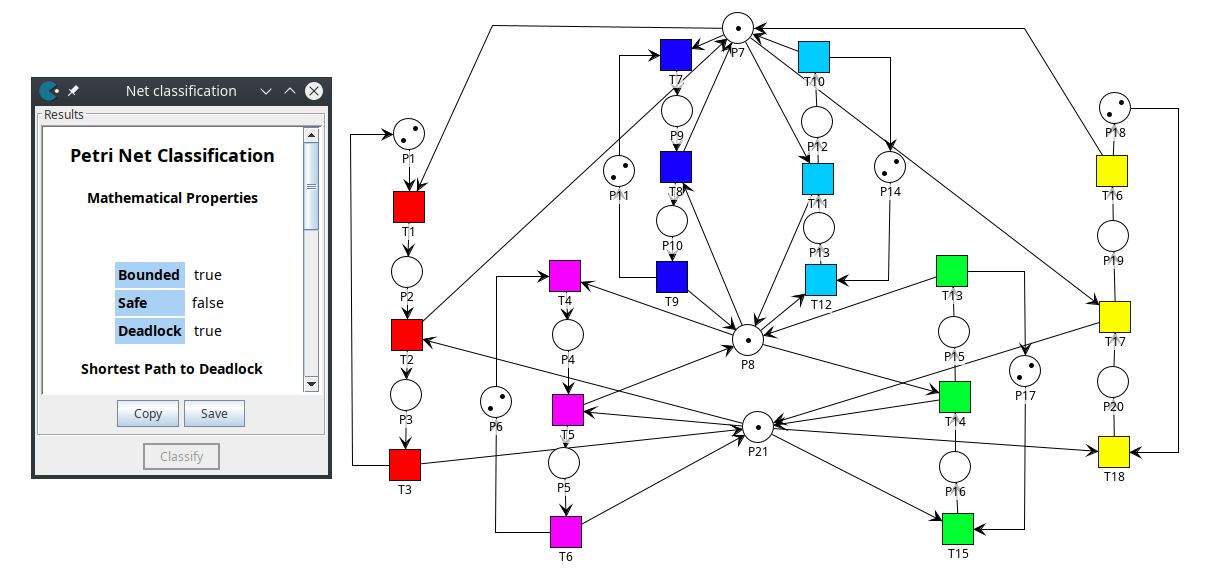
\includegraphics[width=\textwidth]{Figures/testing/auto-t-inv.png}
	\caption[RdP Auto y sus T-invariantes.]{RdP Auto \footnotemark \ y sus T-invariantes.}
	\label{fig:amsinvariantes}
 \end{figure} \footnotetext{Figura adaptada del paper publicado por \textit{Huixia Liu} et al. \cite{paperauto}}

En la figura \ref{fig:amsinvariantes}, se presentan los T-invariantes en diferentes colores. 

\paragraph{Control de la red}
\hfill \break
Al agregar los supervisores en la red ésta aún presentaba deadlock, lo que se hizo fue ejecutar la parte 3 del algoritmo para resolver tanto el problema de conflicto y de t\_idle, logrando de esta manera el control de la red.

\bigskip 
\begin{table}[H]
    \small
    \centering
    \begin{tabular}{|c|c|P{2cm}|P{2.3cm}|P{4.25cm}|}
    \hline
    \textbf{Supervisor} & \textbf{Marcado} & \textbf{Transiciones input} & \textbf{Transiciones output} & \textbf{Bad Siphon Controlado}  \\  \hline
    $P_{22}$ & 1 & \{$T_{2},T_{8},T_{11}, \break T_{13}$\} & \{$T_{1},T_{7},T_{12},T_{15}$\} & \{$P_2, P_5, P_9, P_{10}, P_{13}, P_{17}, \break P_{19}, P_{20}$\} \\ 
    \hline
    $P_{23}$ & 1 & \{$T_{2},T_{13},T_{17}$\} & \{$T_{1},T_{15},T_{18}$\} & \{$P_3, P_6, P_8, P_{10}, P_{14}, P_{17}, \break P_{19}, P_{21}$\} \\ 
    \hline
    $P_{24}$ & 1 & \{$T_{2},T_{5},T_{14}$\} & \{$T_{1},T_{4},T_{15}$\} & \{$P_3, P_6, P_9, P_{11}, P_{13}, P_{16}, \break P_{20}, P_{21}$\} \\ 
    \hline
    $P_{25}$ & 2 & \{$T_{2},T_{5},T_{8}, \break T_{11},T_{14},T_{17}$\} & \{$T_{1},T_{4},T_{7},T_{12}, \break T_{15},T_{18}$\} & \{$P_3, P_6, P_9, P_{10}, P_{13}, P_{17}, \break P_{19}, P_{20}, P_{21}$\} \\
    \hline
    \end{tabular}
    \caption{Supervisores: RdP Auto}
    \label{tab:AMS12-v4}
\end{table}
\hfill

\begin{figure}[H]
	\centering
	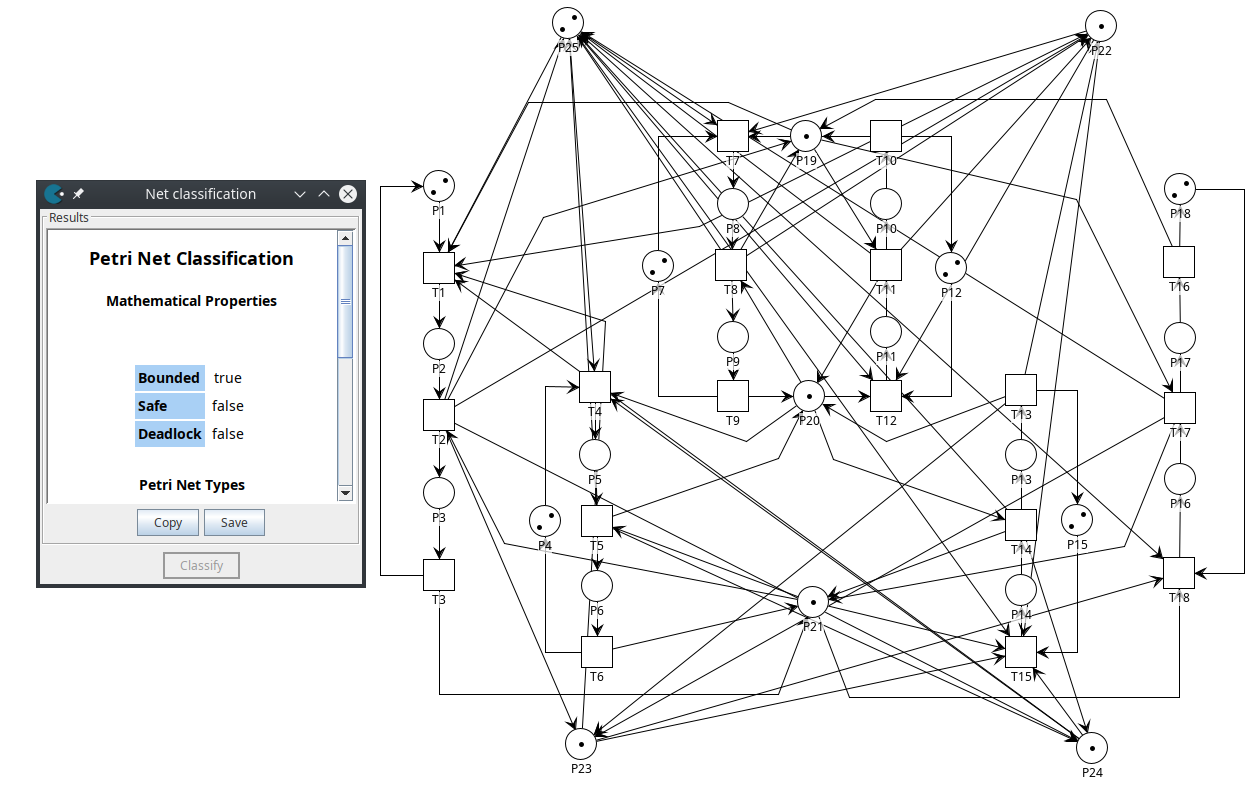
\includegraphics[scale=0.45]{Figures/testing/auto-controlada.png}
	\caption[RdP Auto controlada]{RdP Auto controlada.}
	\label{fig:amscontrolada}
 \end{figure} 

%-------------------------------------------------------------------------------

\subsubsection{Características generales red Hiuxia}
\begin{itemize}
    \item Los recursos de la red están representados por las plazas \{$P_{9},P_{10},P_{11}$\}.
\end{itemize}

\subsubsection{Análisis estructural red Hiuxia}
\hfill
\begin{figure}[H]
	\centering
	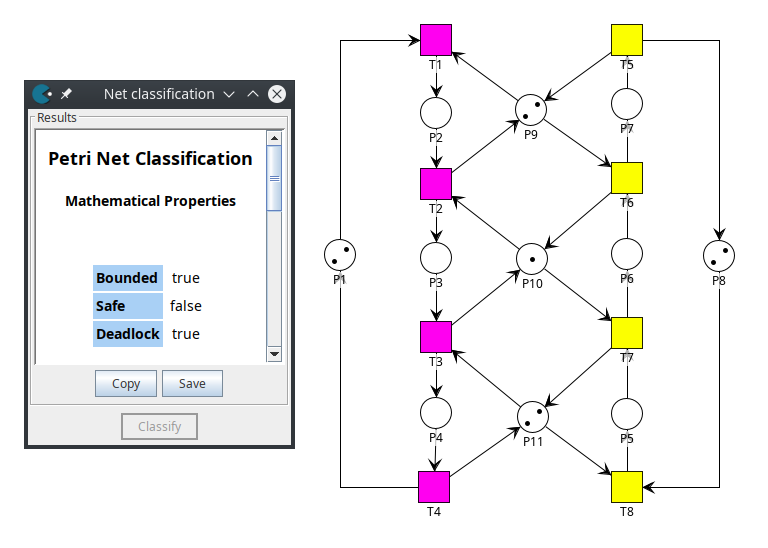
\includegraphics[scale=0.6]{Figures/testing/hiuxia-t-inv.png}
	\caption[RdP Hiuxia y sus T-invariantes.]{RdP Hiuxia \footnotemark \ y sus T-invariantes.}
	\label{fig:hiuxiainvariantes}
 \end{figure} \footnotetext{Figura adaptada del paper publicado por \textit{Huixia Liu} et al. \cite{paperauto}}

En la figura \ref{fig:hiuxiainvariantes}, se presentan los T-invariantes en diferentes colores. \\

\paragraph{Control de la red}
\hfill \break
Para alcanzar la vivacidad de esta red bastó con agregar los supervisores y no fue necesario ejecutar la parte 3 del algoritmo dado que al agregar los mismos se alcanzó el control de la red, eliminando las situaciones de deadlock.

\begin{table}[H]
    \small
    \centering
    \begin{tabular}{|c|c|P{2cm}|P{2.3cm}|c|}
    \hline
    \textbf{Supervisor} & \textbf{Marcado} & \textbf{Transiciones input} & \textbf{Transiciones output} & \textbf{Bad Siphon Controlado}  \\  \hline
    $P_{12}$ & 2 & \{$T_{2},T_{6}$\} & \{$T_{1},T_{8}$\} & \{$P_3, P_7, P_9, P_{10}$\} \\ 
    \hline
    $P_{13}$ & 2 & \{$T_{3}, T_{7}$\} & \{$T_1,T_8$\} & \{$P_4, P_6, P_{10}, P_{11}$\} \\ 
    \hline
    \end{tabular}
    \caption{Supervisores: RdP Hiuxia}
    \label{tab:Hiuxia12-v4}
\end{table}
\hfill

\begin{figure}[H]
	\centering
	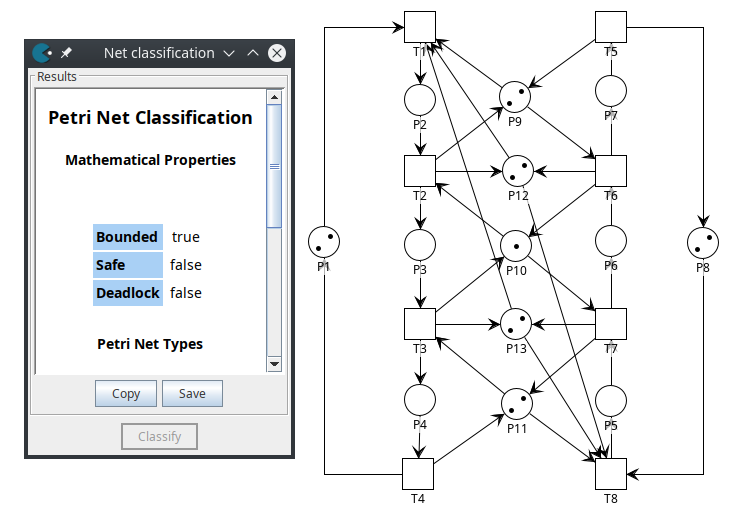
\includegraphics[width=\textwidth]{Figures/testing/hiuxia-controlada.png}
	\caption[RdP Hiuxia controlada]{RdP Hiuxia controlada.}
	\label{fig:hiuxiacontrolada}
 \end{figure} 
 
%-------------------------------------------------------------------------------------

\subsection{Casos YiFan (1,2,3) }
Estas tres redes\footnote{En estas RdP fueron modificados los pesos de los arcos reduciéndolos a uno para adaptarlas al tipo de red que admite el algoritmo.} presentes en el paper de YiFan et al. \cite{paperyifanhou} también son del tipo AMS. Este sistema consiste en un conjunto de estaciones interconectadas para el procesamiento de materiales que es capaz de procesar automáticamente una amplia variedad de tipos de piezas de manera simultánea y controlada por computadoras.\\
Un AMS tiene características de alto grado de automatización, de integración y de flexibilidad. 
En las redes existen ciertas plazas que simulan la disponibilidad de recursos y un control incorrecto de estos en la ejecución de los procesos de trabajo, puede conducir a situaciones de deadlock.

\subsubsection{Características generales YiFan1}
\begin{itemize}
    \item Los recursos de la red están representados por las plazas \{$P_{12},P_{13},P_{14}, P_{15}$\}.
\end{itemize}

\subsubsection{Análisis estructural YiFan1}
\hfill
\begin{figure}[H]
	\centering
	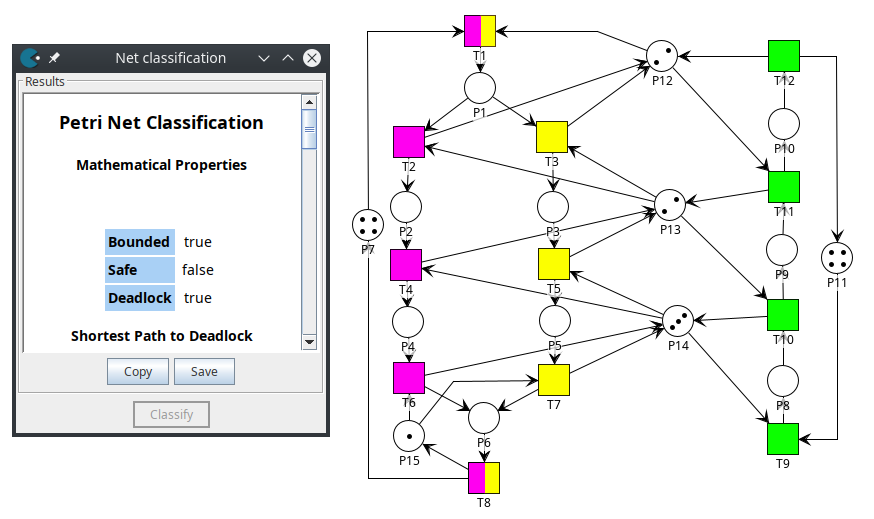
\includegraphics[width=\textwidth]{Figures/testing/yifan1_tinvariantes.png}
	\caption[RdP YiFan1 y sus T-invariantes.]{RdP YiFan1 \footnotemark \ y sus T-invariantes.}
	\label{fig:yifan1_invariantes}
 \end{figure} \footnotetext{Figura adaptada del paper publicado por \textit{YiFan Hou} et al. \cite{paperyifanhou}}

En la figura \ref{fig:yifan1_invariantes}, se presentan los diferentes T-invariantes en diferentes colores. \\

\paragraph{Control de la red}
\hfill \break
Para alcanzar la vivacidad de esta red bastó con agregar los supervisores y no fue necesario ejecutar la parte 3 del algoritmo dado que al agregar los mismos se alcanzó el control de la red, eliminando las situaciones de deadlock.

\bigskip
\begin{table}[H]
    \small
    \centering
    \begin{tabular}{|c|c|P{2cm}|P{2.3cm}|c|}
    \hline
    \textbf{Supervisor} & \textbf{Marcado} & \textbf{Transiciones input} & \textbf{Transiciones output} & \textbf{Bad Siphon Controlado}  \\  \hline
    $P_{16}$ & 3 & \{$T_{2},T_{3},T_{11}$\} & \{$T_{1},T_{9}$\} & \{$P_2, P_3, P_{10}, P_{12}, P_{13}$\} \\ 
    \hline
    $P_{17}$ & 4 & \{$T_{4}, T_{5}, T_{10}$\} & \{$T_1,T_9$\} & \{$P_4, P_5, P_{9}, P_{13}, P_{14}$\} \\ 
    \hline
    \end{tabular}
    \caption{Supervisores: RdP YiFan1}
    \label{tab:Yifan1}
\end{table}
\hfill

\begin{figure}[H]
	\centering
	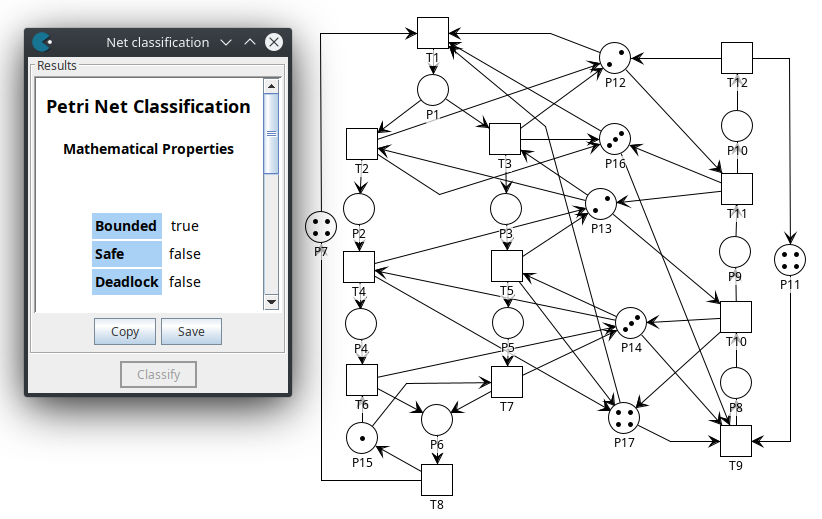
\includegraphics[width=\textwidth]{Figures/testing/yifan1_controlada.png}
	\caption[RdP YiFan1 controlada]{RdP YiFan1 controlada.}
	\label{fig:yifan1controlada}
 \end{figure}
 
 %-------------------------------------------------------------------------------------
\subsubsection{Características generales YiFan2}
\begin{itemize}
    \item Los recursos de la red están representados por las plazas \{$P_{11},P_{12},P_{13}$\}.
\end{itemize}

\subsubsection{Análisis estructural YiFan2}
\hfill
\begin{figure}[H]
	\centering
	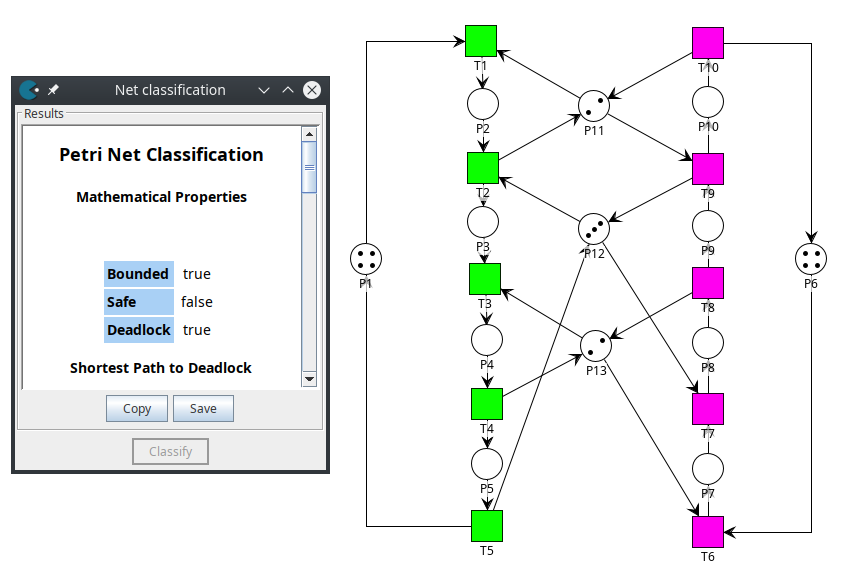
\includegraphics[width=\textwidth]{Figures/testing/yifan2_tinvariantes.png}
	\caption[RdP YiFan2 y sus T-invariantes.]{RdP YiFan2 \footnotemark \ y sus T-invariantes.}
	\label{fig:yifan2_invariantes}
 \end{figure} \footnotetext{Figura adaptada del paper publicado por \textit{YiFan Hou} et al. \cite{paperyifanhou}}

En la figura \ref{fig:yifan2_invariantes}, se presentan los T-invariantes en diferentes colores. \\


\paragraph{Control de la red}
\hfill \break
Para alcanzar la vivacidad de esta red bastó con agregar los supervisores y no fue necesario ejecutar la parte 3 del algoritmo dado que al agregar los mismos se alcanzó el control de la red, eliminando las situaciones de deadlock.
\begin{table}[H]
    \small
    \centering
    \begin{tabular}{|c|c|P{2cm}|P{2.3cm}|c|}
    \hline
    \textbf{Supervisor} & \textbf{Marcado} & \textbf{Transiciones input} & \textbf{Transiciones output} & \textbf{Bad Siphon Controlado}  \\  \hline
    $P_{14}$ & 6 & \{$T_{4},T_{9}$\} & \{$T_{1},T_{6}$\} & \{$P_4, P_5, P_8, P_{10}, P_{11}, P_{12}, P_{13}$\} \\ 
    \hline
    $P_{15}$ & 4 & \{$T_{4}, T_{8}$\} & \{$T_1,T_6$\} & \{$P_4, P_5, P_{8}, P_{9}, P_{12}, P_{13}$\} \\ 
    \hline
    $P_{16}$ & 4 & \{$T_{2}, T_{9}$\} & \{$T_1,T_6$\} & \{$P_3, P_4, P_{5}, P_{10}, P_{11}, P_{12}$\} \\
    \hline
    \end{tabular}
    \caption{Supervisores: RdP YiFan2}
    \label{tab:Yifan2}
\end{table}
\hfill

\begin{figure}[H]
	\centering
	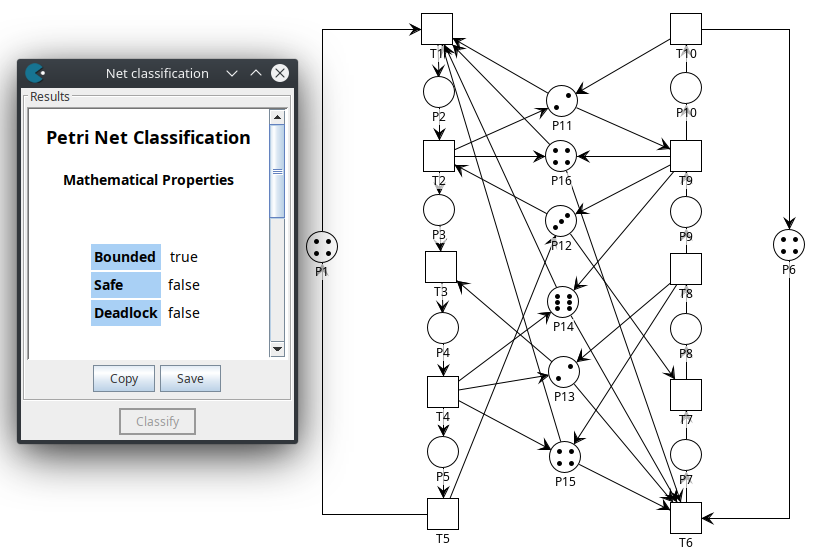
\includegraphics[width=\textwidth]{Figures/testing/yifan2_controlada.png}
	\caption[RdP YiFan2 controlada]{RdP YiFan2 controlada.}
	\label{fig:yifan2controlada}
 \end{figure}
 
 %-------------------------------------------------------------------------------------
\subsubsection{Características generales YiFan3}
\begin{itemize}
    \item Los recursos de la red están representados por las plazas \{$P_{5},P_{6}$\}.
\end{itemize}

\subsubsection{Análisis estructural YiFan3}
\hfill
\begin{figure}[H]
	\centering
	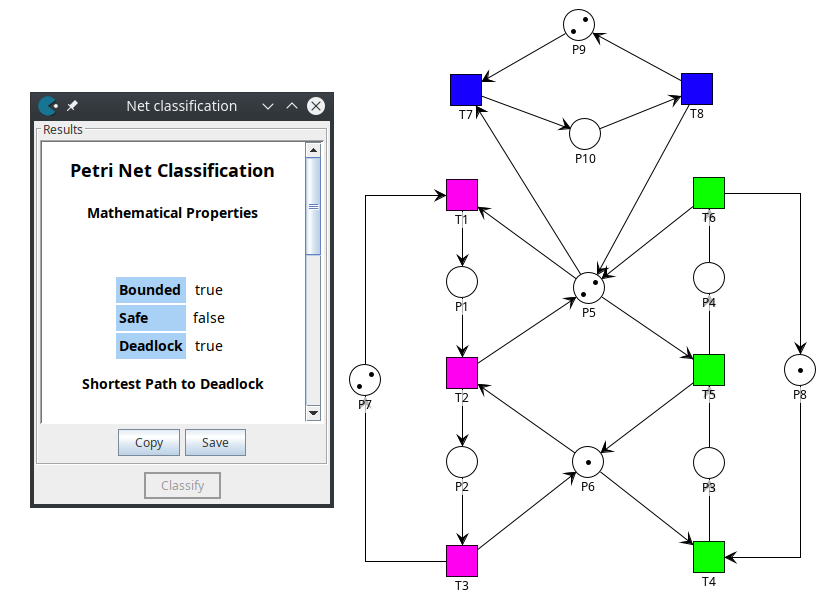
\includegraphics[width=\textwidth]{Figures/testing/yifan3_tinvariantes.png}
	\caption[RdP YiFan3 y sus T-invariantes.]{RdP YiFan3 \footnotemark \ y sus T-invariantes.}
	\label{fig:yifan3invariantes}
 \end{figure} \footnotetext{Figura adaptada del paper publicado por \textit{YiFan Hou} et al. \cite{paperyifanhou}}

En la figura \ref{fig:yifan3invariantes}, se presentan los T-invariantes en diferentes colores. \\

\paragraph{Control de la red}
\hfill \break
Al agregar los supervisores en la red ésta aún presentaba deadlock, lo que se hizo fue ejecutar la parte 3 del algoritmo para resolver tanto el problema de conflicto y de t\_idle, logrando de esta manera el control de la red.
\begin{table}[H]
    \small
    \centering
    \begin{tabular}{|c|c|P{2cm}|P{2.3cm}|c|}
    \hline
    \textbf{Supervisor} & \textbf{Marcado} & \textbf{Transiciones input} & \textbf{Transiciones output} & \textbf{Bad Siphon Controlado}  \\  \hline
    $P_{11}$ & 2 & \{$T_{2},T_{5}$\} & \{$T_{1},T_{4}$\} & \{$P_2, P_4, P_5,P_6, P_{10}$\} \\ 
    \hline
    \end{tabular}
    \caption{Supervisores: RdP YiFan3}
    \label{tab:Yifan3}
\end{table}
\hfill

\begin{figure}[H]
	\centering
	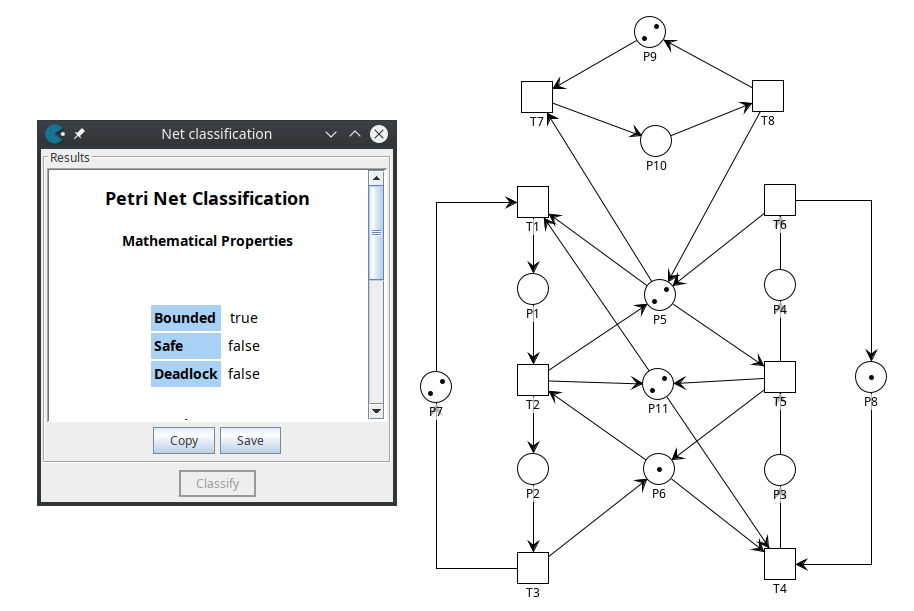
\includegraphics[width=\textwidth]{Figures/testing/yifan3_controlada.png}
	\caption[RdP YiFan3 controlada]{RdP YiFan3 controlada.}
	\label{fig:yifan3controlada}
 \end{figure}
 
 %-------------------------------------------------------------------------------------
\subsection{Caso JianChao}
Esta red modela la ejecución concurrente de un AMS, se presentan dos procesos productivos que comparten compuesto por 4 robot y 6 maquinas. Un control incorrecto de estos en la ejecución de los procesos de trabajo, puede conducir a situaciones de deadlock.\\

% \begin{figure}[H]
% 	\centering
% 	\includegraphics[width=\textwidth]{Figures/testing/jianchaomodelado.png}
% 	\caption[Modelado RdP JianChao.]{Modelado RdP JianChao \footnotemark \.}
% 	\label{fig:modeladoJianchao}
%  \end{figure} \footnotetext{Figura adaptada del paper publicado por \textit{H. Liu} et al. \cite{JianchaoModelado}}

\subsubsection{Características generales}
\begin{itemize}
    \item Los robot de la red están representados por las plazas \{$P_{20}, P_{22}, P_{24}, P_{26}$\}.
    \item Las maquinas de la red están representados por las plazas \{$P_{21}, P_{23}, P_{25}, P_{27}, P_{28}, P_{29}$\}.
\end{itemize}

\subsubsection{Análisis estructural}
\hfill
\begin{figure}[H]
	\centering
	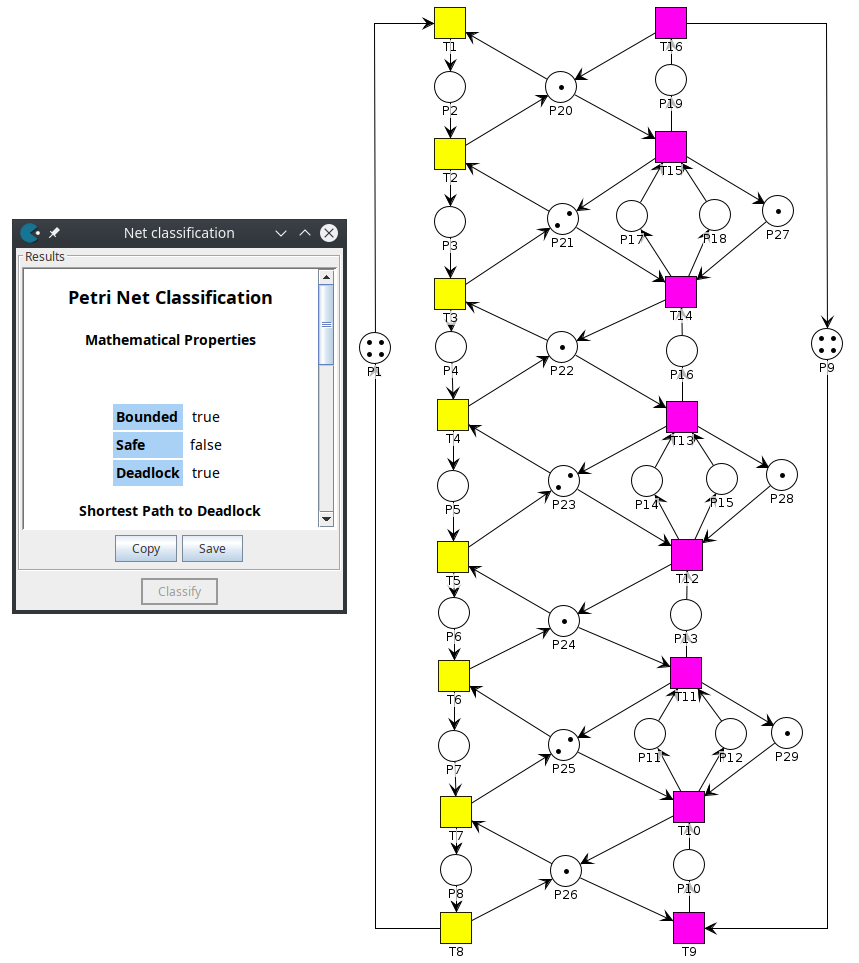
\includegraphics[width=\textwidth]{Figures/testing/jianchaodeadlock.png}
	\caption[RdP JianChao y sus T-invariantes.]{RdP JianChao \footnotemark \ y sus T-invariantes.}
	\label{fig:jianchaoinvariantes}
 \end{figure} \footnotetext{Figura adaptada del paper publicado por \textit{JianChao Lou} et al. \cite{paperjianchao}}

En la figura \ref{fig:jianchaoinvariantes} \footnote{En esta RdP fue modificado el peso de los arcos reduciéndolos a uno para adaptarlas al tipo de red que admite el algoritmo.}, se presentan los T-invariantes en diferentes colores.\\

\paragraph{Control de la red}
\hfill \break
Para alcanzar la vivacidad de esta red bastó con agregar los supervisores y no fue necesario ejecutar la parte 3 del algoritmo dado que al agregar los mismos se alcanzó el control de la red, eliminando las situaciones de deadlock.
\begin{table}[H]
    \small
    \centering
    \begin{tabular}{|c|c|P{2cm}|P{2.3cm}|c|}
    \hline
    \textbf{Supervisor} & \textbf{Marcado} & \textbf{Transiciones input} & \textbf{Transiciones output} & \textbf{Bad Siphon Controlado}  \\  \hline
    $P_{30}$ & 2 & \{$T_{7},T_{10}$\} & \{$T_{1},T_{9}$\} & \{$P_8, P_{11}, P_{25}, P_{26}$\} \\ 
    \hline
    $P_{31}$ & 2 & \{$T_{5}, T_{12}$\} & \{$T_1,T_9$\} & \{$P_6, P_{14}, P_{23}, P_{24}$\} \\ 
    \hline
    $P_{32}$ & 2 & \{$T_{3}, T_{14}$\} & \{$T_1,T_9$\} & \{$P_4, P_{17}, P_{21}, P_{22}$\} \\ 
    \hline
    \end{tabular}
    \caption{Supervisores: RdP JianChao}
    \label{tab:Jianchao}
\end{table}
\hfill

\begin{figure}[H]
	\centering
	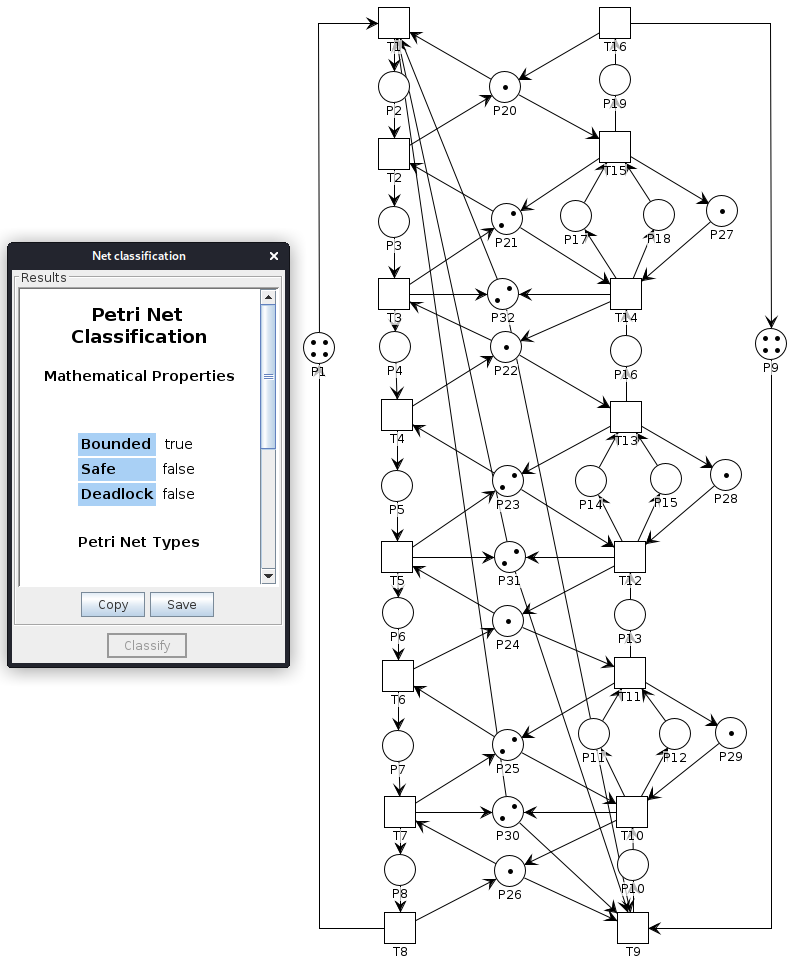
\includegraphics[width=\textwidth]{Figures/testing/jianchao_controlada.png}
	\caption[RdP JianChao controlada]{RdP JianChao controlada.}
	\label{fig:jianchaocontrolada}
 \end{figure}

%-------------------------------------------------------------------------------------

\subsection{Caso Zhiwuli}
Esta red modela la ejecución concurrente de un FMS. El mismo consta de 3 procesos productivos que comparten 2 recursos y un control incorrecto de estos en la ejecución de los procesos de trabajo, puede conducir a situaciones de deadlock.

\subsubsection{Características generales}
\begin{itemize}
    \item Los recursos de la red están representados por las plazas \{$P_{7},P_{8}$\}.
\end{itemize}

\subsubsection{Análisis estructural}
\hfill
\begin{figure}[H]
	\centering
	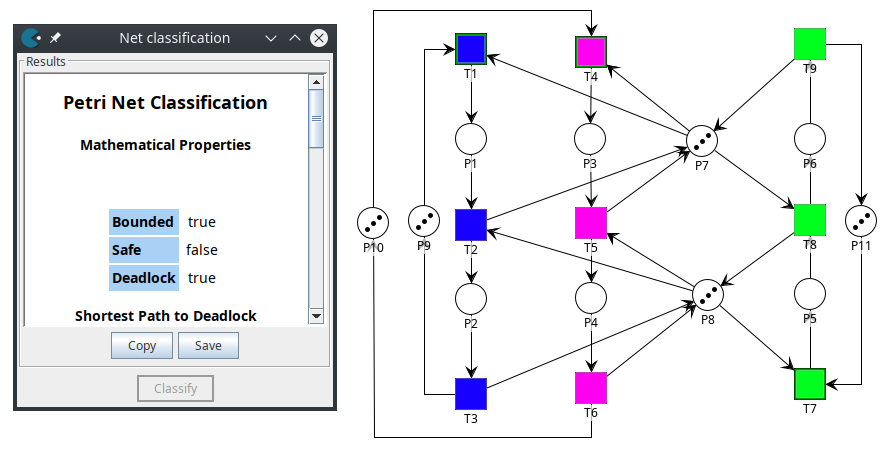
\includegraphics[width=\textwidth]{Figures/testing/zhiwuli_tinvariantes.png}
	\caption[RdP Zhiwuli y sus T-invariantes.]{RdP Zhiwuli \footnotemark \ y sus T-invariantes.}
	\label{fig:zhiwuli_tivariantes}
 \end{figure} \footnotetext{Figura adaptada del paper publicado por \textit{ZhiWu Li} et al. \cite{paperzhiwuli}}

En la figura \ref{fig:zhiwuli_tivariantes} \footnote{En esta RdP fue modificado el peso de los arcos reduciéndolos a uno (1) para adaptarla al tipo de red que admite el algoritmo.}, se presentan los T-invariantes en diferentes colores. \\

\paragraph{Control de la red}
\hfill \break
Para alcanzar la vivacidad de esta red bastó con agregar los supervisores y no fue necesario ejecutar la parte 3 del algoritmo dado que al agregar los mismos se alcanzó el control de la red, eliminando las situaciones de deadlock.

\bigskip
\begin{table}[H]
    \small
    \centering
    \begin{tabular}{|c|c|P{2cm}|P{2.3cm}|c|}
    \hline
    \textbf{Supervisor} & \textbf{Marcado} & \textbf{Transiciones input} & \textbf{Transiciones output} & \textbf{Bad Siphon Controlado}  \\  \hline
    $P_{12}$ & 5 & \{$T_{2}, T_5, T_{8}$\} &  \{$T_{1},T_{4}, T_7$\} & \{$P_2, P_4, P_6, P_7, P_8$\} \\ 
    \hline
    \end{tabular}
    \caption{Supervisores: RdP Zhiwuli}
    \label{tab:Zhiwuli}
\end{table}
\hfill

\begin{figure}[H]
	\centering
	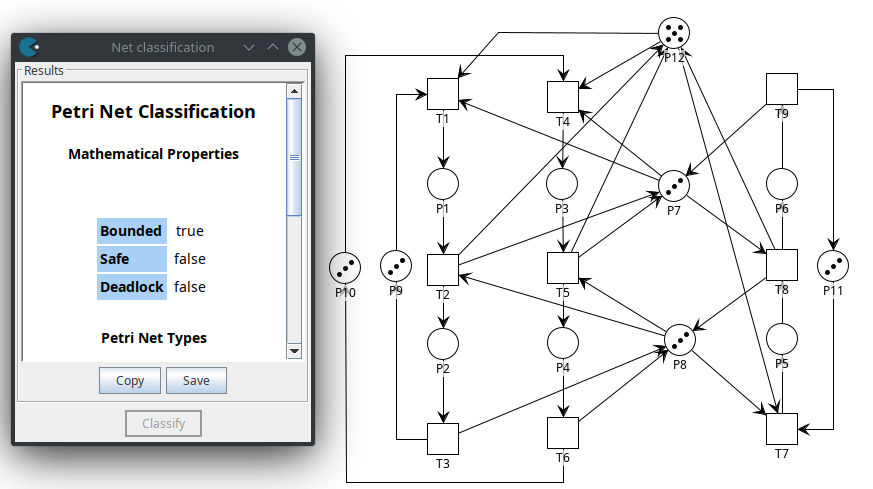
\includegraphics[width=\textwidth]{Figures/testing/zhiwuli_controlada.png}
	\caption[RdP Zhiwuli controlada]{RdP Zhiwuli controlada.}
	\label{fig:zhiwulicontrolada}
 \end{figure}
 
 %-------------------------------------------------------------------------------------
 
\subsection{Caso Fanti}
La red representa un AMS, la cual consta de un conjunto de estaciones de trabajo, cada una de las cuales es capaz de procesar piezas de diferente tipo de acuerdo con una secuencia de operaciones prescrita. Para el desarrollo de estas piezas la red presenta 4 recursos compartidos y una mala gestión de los mismos desencadenará el bloqueo de la red.

\subsubsection{Características generales}
\begin{itemize}
    \item Los recursos de la red están representados por las plazas \{$P_{10},P_{11},P_{12},P_{13}$\}.
\end{itemize}

\subsubsection{Análisis estructural}
\hfill
\begin{figure}[H]
	\centering
	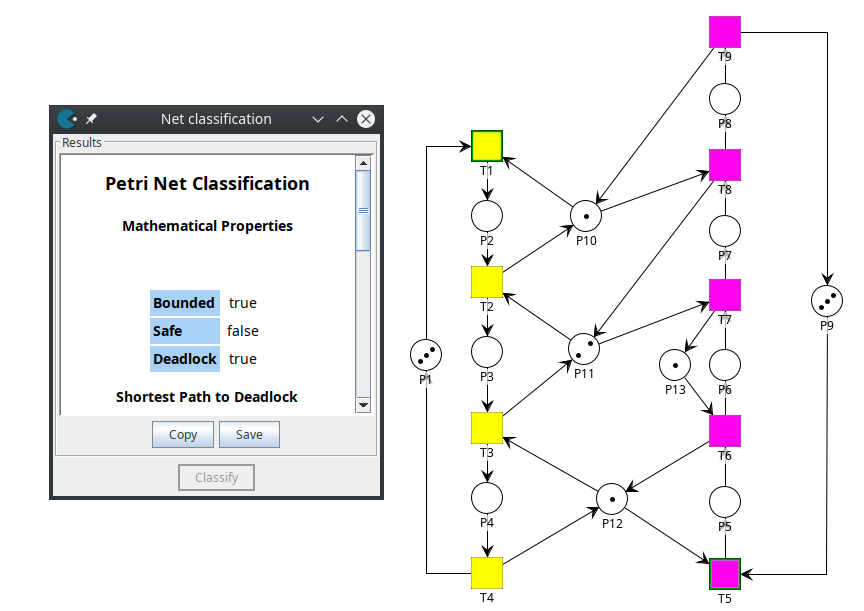
\includegraphics[width=\textwidth]{Figures/testing/fanti_tinvariantes.png}
	\caption[RdP Fanti y sus T-invariantes.]{RdP Fanti \footnotemark \ y sus T-invariantes.}
	\label{fig:fanti_tinvariantes}
 \end{figure} \footnotetext{Figura adaptada del paper publicado por \textit{Fanti} et al. \cite{paperfanti}}

En la figura \ref{fig:fanti_tinvariantes} , se presentan los T-invariantes en diferentes colores.\\

\paragraph{Control de la red}
\hfill \break
Para alcanzar la vivacidad de esta red bastó con agregar los supervisores y no fue necesario ejecutar la parte 3 del algoritmo dado que al agregar los mismos se alcanzó el control de la red, eliminando las situaciones de deadlock.
\begin{table}[H]
    \small
    \centering
    \begin{tabular}{|c|c|P{2cm}|P{2.3cm}|c|}
    \hline
    \textbf{Supervisor} & \textbf{Marcado} & \textbf{Transiciones input} & \textbf{Transiciones output} & \textbf{Bad Siphon Controlado}  \\  \hline
    $P_{14}$ & 4 & \{$T_{3},T_{8}$\} & \{$T_{1},T_{5}$\} & \{$P_4, P_8, P_{10}, P_{11}, P_{12}, P_{13} $\} \\ 
    \hline
    $P_{15}$ & 2 & \{$T_{2}, T_{8}$\} & \{$T_1,T_5$\} & \{$P_3, P_8, P_{10}, P_{11}$\} \\ 
    \hline
    $P_{16}$ & 3 & \{$T_{3}, T_{7}$\} & \{$T_1,T_5$\} & \{$P_4, P_7, P_{11}, P_{12}, P_{13}$\} \\ 
    \hline
    \end{tabular}
    \caption{Supervisores: RdP Fanti}
    \label{tab:fanti}
\end{table}
\hfill

\begin{figure}[H]
	\centering
	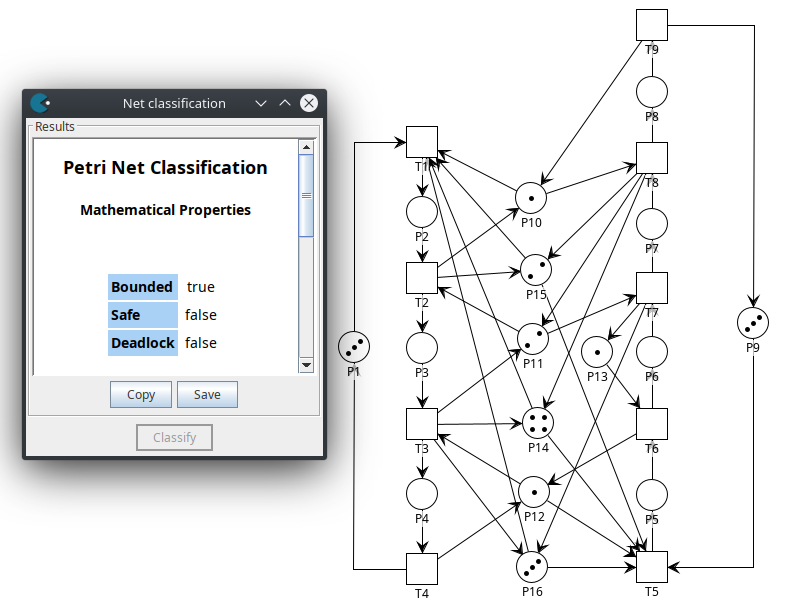
\includegraphics[width=\textwidth]{Figures/testing/fanti_controlada.png}
	\caption[RdP Fanti controlada]{RdP Fanti controlada.}
	\label{fig:fanticontrolada}
 \end{figure}
 
%-------------------------------------------------------------------------------------
\subsection{Caso Hesuan Hu}
La red representa un AMS donde se fabrican tres tipos de productos. El sistema esta compuesto por seis robots y cinco maquinas, cada uno de estos puede contener un solo producto.

 \subsubsection{Características generales}
\begin{itemize}
    \item Los robots de la red están representados por las plazas \{$P_{20},P_{22},P_{23},P_{30},P_{33},P_{35},$\}.
    \item Las máquinas de la red están representados por las plazas \{$P_{8},P_{9},P_{21},P_{31},P_{32}$\}.
    \item El primer producto comienza con la ejecución de la {$T_1$} y finaliza con la {$T_4$}.
    \item El segundo producto comienza con la ejecución de la {$T_9$} y finaliza con la {$T_{14}$}.
    \item El tercer producto comienza con la ejecución de la {$T_{19}$} y finaliza con la {$T_{24}$}.
\end{itemize}

\subsubsection{Análisis estructural}
\hfill
\begin{figure}[H]
	\centering
	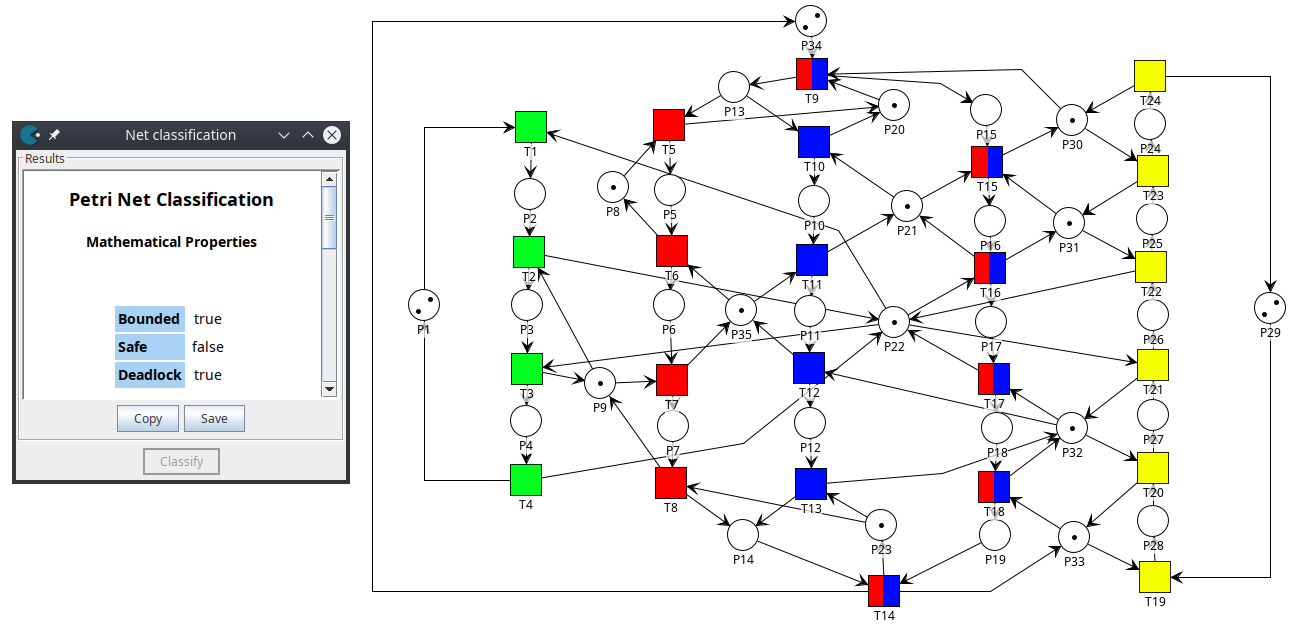
\includegraphics[width=\textwidth]{Figures/testing/fig3_deadlock.png}
	\caption[RdP Hesuan Hu y sus T-invariantes.]{RdP Hesuan Hu \footnotemark \ y sus T-invariantes.}
	\label{fig:hesuan_hu_tinvariantes}
 \end{figure} \footnotetext{Figura adaptada del paper publicado por \textit{Hesuan Hu} et al. \cite{paperhu}}

En la figura \ref{fig:hesuan_hu_tinvariantes} \footnote{En esta RdP fue modificado el peso de los arcos reduciéndolos a uno para adaptarlas al tipo de red que admite el algoritmo.}, se presentan los T-invariantes en diferentes colores.\\

\paragraph{Control de la red}
\hfill \break
Al agregar los supervisores en la red ésta aún presentaba deadlock, lo que se hizo fue ejecutar la parte 3 del algoritmo para resolver tanto el problema de conflicto y de t\_idle, logrando de esta manera el control de la red.
\begin{table}[H]
    \small
    \centering
    \begin{tabular}{|c|c|P{2.4cm}|P{2.2cm}|P{4.2cm}|}
    \hline
    \textbf{Supervisor} & \textbf{Marcado} & \textbf{Transiciones input} & \textbf{Transiciones output} & \textbf{Bad Siphon Controlado}  \\  \hline
    $P_{36}$ & 2 & \{$T_{3},T_{16},T_{22}$\} & \{$T_{1},T_{9},T_{19}$\} & \{$P_4, P_7, P_{9}, P_{17}, P_{22}, P_{25}, P_{31} $\} \\ 
    \hline
    $P_{37}$ & 1 & \{$T_{17}, T_{21}$\} & \{$T_9,T_{19}$\} & \{$P_2, P_4, P_{12}, P_{18}, P_{22}, P_{26}, P_{32}$\} \\ 
    \hline
    $P_{38}$ & 3 & \{$T_{3}, T_{8}, T_{13}, T_{21}$\} & \{$T_1,T_9, T_{19}$\} & \{$P_4, P_7, P_{9}, P_{12}, P_{14}, P_{22}, P_{26}, \break P_{32}, P_{33}$\} \\ 
    \hline
    $P_{39}$ & 1 & \{$T_{3}$\} & \{$T_1$\} & \{$P_4, P_7, P_{9}, P_{17}, P_{22}, P_{26}$\} \\ 
    \hline
    $P_{40}$ & 1 & \{$T_{16}, T_{22}$\} & \{$T_9,T_{19}$\} & \{$P_2, P_4, P_{17}, P_{22}, P_{25}, P_{31}$\} \\ 
    \hline
    \end{tabular}
    \caption{Supervisores: RdP Hesuan Hu}
    \label{tab:hu}
\end{table}
\hfill

\begin{figure}[H]
	\centering
	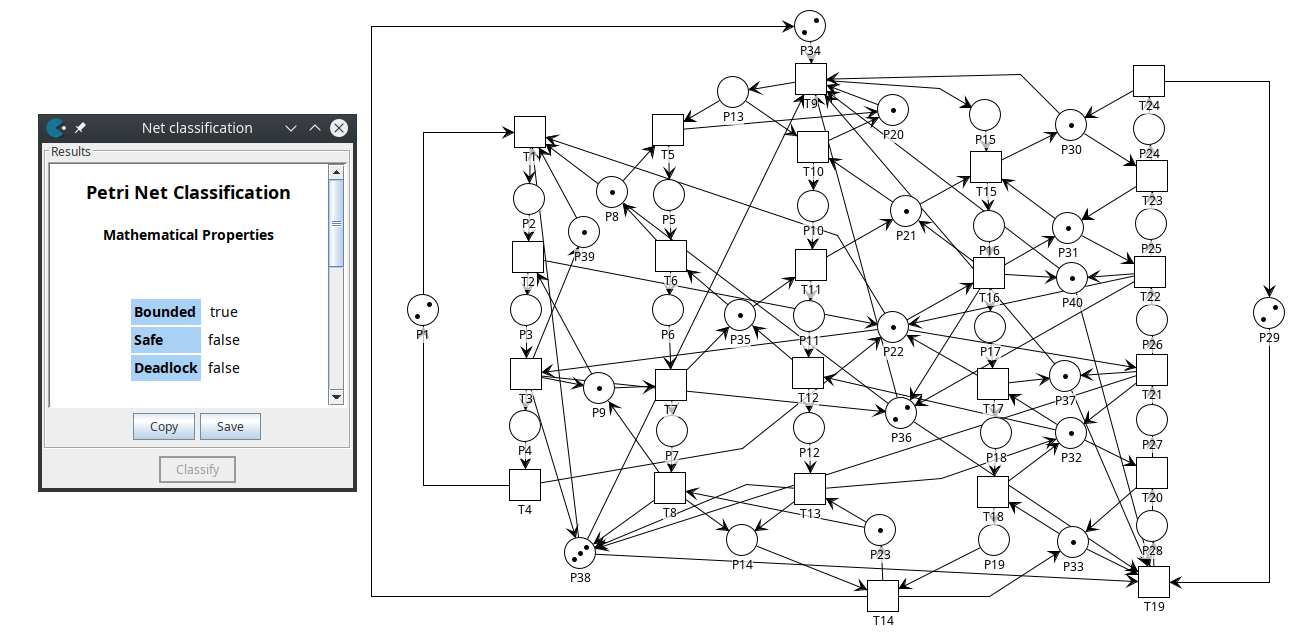
\includegraphics[width=\textwidth]{Figures/testing/fig3_sindeadlock.png}
	\caption[RdP Hesuan Hu controlada]{RdP Hesuan Hu controlada.}
	\label{fig:hucontrolada}
 \end{figure}
 % Chapter Template

\chapter{Conclusión} % Main chapter title

\label{Chapter7} % Change X to a consecutive number; for referencing this chapter elsewhere, use \ref{ChapterX}
En el capítulo introductorio del presente documento se especificaron los objetivos planteados para el proyecto desarrollado. Una vez finalizadas las tareas asociadas a los mismos, es posible extraer algunas conclusiones. \\

Por un lado se logró establecer una retroalimentación entre nuestro algoritmo y el software Petrinator, como ya se mencionó con anterioridad, en lo que sería la extracción manual de los archivos y su posterior procesamiento; así como también la actualización de la red con sus respectivos supervisores. \\

Por otra parte, se detectó la necesidad de extraer los T-invariantes de la red original, dado que estos debían preservarse a lo largo del análisis ya que con la incorporación de un nuevo supervisor la estructura de la red se ve afectada pudiendo perder los mismos, alterando el análisis y el objetivo es conservar el comportamiento de la red, es decir, que mantenga sus T-invariantes (que los procesos se sigan ejecutando de la misma manera) pero de una forma controlada y manteniendo la concurrencia de los procesos. \\
Esta modificación estructural que se presenta en la red es producto del nuevo supervisor, ya que al colocarlo no se tiene en cuenta si la red presenta conflictos o si las transiciones idle que le extraen el token son realmente necesarias. Para el primero se verificó que si la red presentaba conflictos antes de finalizar ese camino el token debía regresar el supervisor. Para el segundo se verificó que la transición idle le quitara token a los supervisores que realmente afectan al proceso que esta transición iba a desencadenar, de no ser así ese arco no debiera existir. \\

A partir de lo mencionado y demostrado a lo largo de la evolución del algoritmo, este se fue probando en redes con estructuras diferentes (conflictos presentes en la red, la distribución/relación entre los bad siphons y los T-invariantes) que permitió demostrar fiabilidad del mismo como también agregarle nuevas características para llegar al objetivo planteado. \\
De esta forma el algoritmo puede ser tomado como base para el estudio y posterior desarrollo en el área de control de redes de Petri.

\newpage
\section{Trabajo a futuro} \label{trabajofuturo}
A continuación se listan los posibles avances que se podría realizar para continuar este proyecto:

\begin{itemize}
    \item Integrar este algoritmo como una nueva funcionalidad del software Petrinator permitiendo la ejecución automática del mismo sin necesidad de la extracción manual de archivos.
    
    \item Posibilidad de integrar este proyecto junto con los que también se están desarrollando en el LAC con la idea de lograr tanto el control de la red como la ejecución de la misma (tanto en hardware como en software) a partir de ciertas políticas definidas. 
    
    \item Posibilidad de realizar un análisis para la determinación de un criterio de elección óptimo del orden de supervisores a colocar para el control de las diferentes redes permitiendo el mayor paralelismo a la hora de ejecutar las mismas. 
    
%    \item Automatizar la tarea de incorporar/eliminar los arcos indicados por el análisis \textit{Red  con supervisores, tratamiento de conflictos y t\_idle} que actualmente se realiza manualmente.
    
    \item Realizar un generador aleatorio de redes de Petri que sirvan de entrada para el algoritmo.
    
    \item Se propone seguir investigando y testeando con nuevos tipos de redes bloqueadas que presenten diferentes características a las ya analizadas.
    
\end{itemize}



%----------------------------------------------------------------------------------------
%	THESIS CONTENT - APPENDICES
%----------------------------------------------------------------------------------------

\appendix % Cue to tell LaTeX that the following "chapters" are Appendices

% Include the appendices of the thesis as separate files from the Appendices folder
% Uncomment the lines as you write the Appendices

% Appendix Template

\chapter{Tutorial de como utilizar el software \textit{Petrinator}} % Main appendix title

\label{AppendixA} % Change X to a consecutive letter; for referencing this appendix elsewhere, use \ref{AppendixX}
En este apéndice, se detalla el procedimiento en el cual se crean y cargan redes de Petri para trabajar con ellas con dicho software.
Luego se explica el procedimiento que se debe seguir para extraer los datos necesarios para el análisis del algortimo.


\section{Ejecución del software}

A continuación explican los pasos que se deben seguir para poder iniciar el agente \textit{Petrinator} en el dispositivo. 

\begin{itemize}   
    \item  \textbf{Ingreso al programa:}
    desde la terminal de linux \footnote{La ejecución del software tambien puede realizarse en Windows. Para ambos casos es necesario instalar los paquetes correspondientes de java.} se ejecuta el comando: 
    \begin{lstlisting}[language=SHELXL]
    		$ java -jar Petrinator.jar
    \end{lstlisting}
    
    \begin{figure} [H]
        \centering
        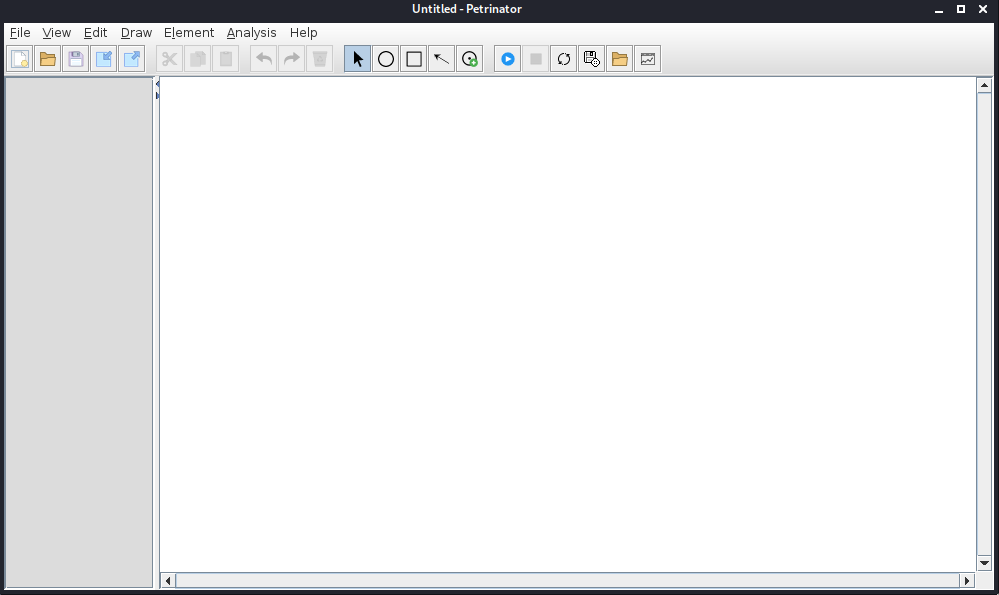
\includegraphics[width=\textwidth]{Figures/petrinator/petrinator-init.png}
        \caption{Software Petrinator .}
        \label{fig:pet-init}
    \end{figure}
   
    \item \textbf{Cargar la red de Petri:} una vez ejecutado exitosamente, se deberá importar o crear la red a analizar. Como se muestra en la figura \ref{fig:file-open}.
    
	\begin{figure} [H]
        \centering
        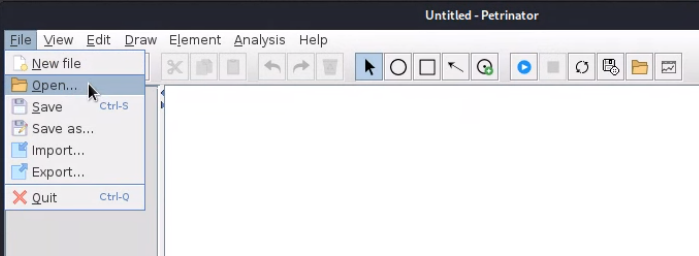
\includegraphics[scale=0.72]{Figures/petrinator/open2.png}
        \caption{Abrir un archivo .}
        \label{fig:pet-open}
    \end{figure} 
    
    \noindent Seleccionar el archivo de extensión \textit{.pflow} a cargar
    \begin{figure} [H]
        \centering
        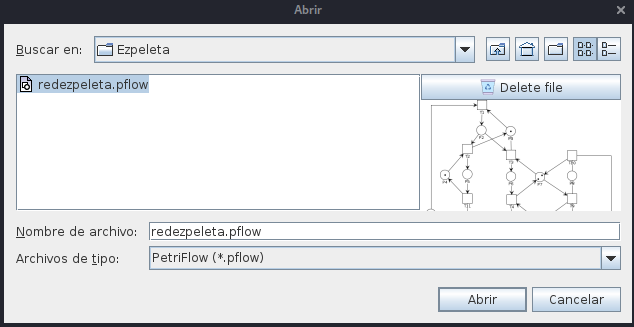
\includegraphics[scale=0.7]{Figures/petrinator/open-example.png}
        \caption{Ventana de selección de archivo .pflow .}
        \label{fig:file-open}
    \end{figure}
    
    \begin{figure} [H]
        \centering
        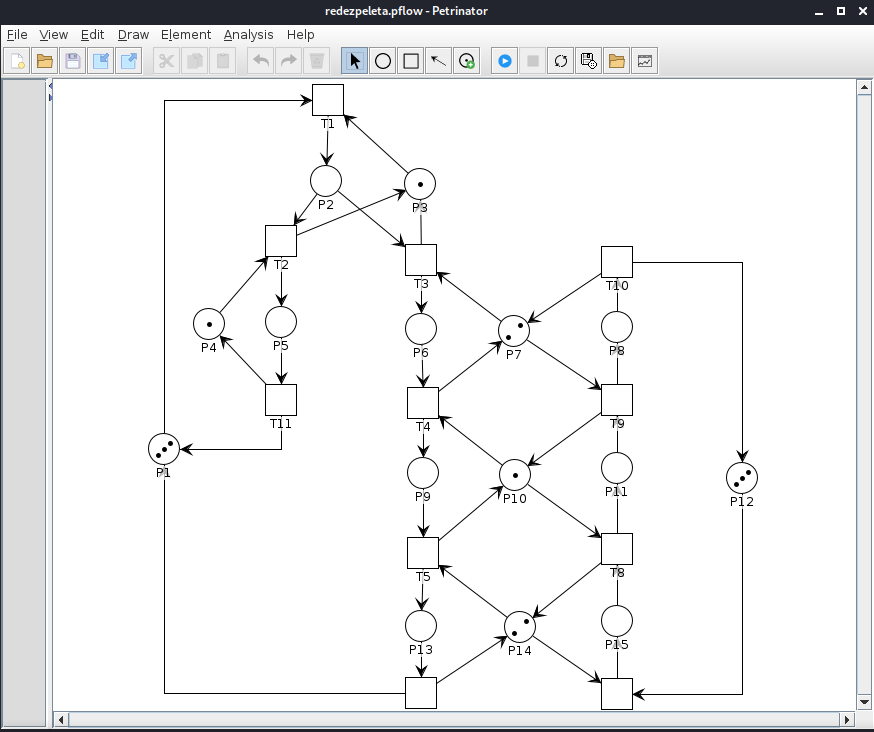
\includegraphics[scale=0.45]{Figures/petrinator/open-example2.png}
        \caption{Red cargada .}
        \label{fig:red-open}
    \end{figure}
    
	
    \item \textbf{Extraer archivos para el análisis:} Como se puede observar en la figura \ref{fig:open-analysis}, en la barra de menú se encuentra la opción de \textit{Analysis} desde donde se pueden realizar los diferentes tipos de análisis en las redes de Petri. A partir de estos, se extraen 4 diferentes archivos.
    
    \begin{figure} [H]
        \centering
        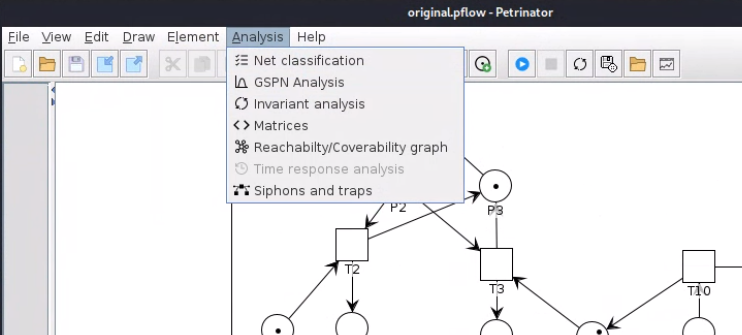
\includegraphics[scale=0.7]{Figures/petrinator/analisis.png}
        \caption{Submenú de análisis.}
        \label{fig:open-analysis}
    \end{figure}
    
    \begin{itemize}
        \item \textbf{Clasificación de la red}: como se observa en la figura \ref{fig:open-analysis} se encuentra en el submenú la opción \textit{Net classification} que nos permite realizar este análisis.
        Una vez seleccionada la opción, se abre una nueva ventana como muestra la figura \ref{fig:clasificacion-red} en dónde se debe pulsar en \textit{Classify} para que el software haga dicho análisis. Para la funcionalidad de nuestro algoritmo no es necesario exportar este archivo, sin embargo es de imprescindible verificar la presencia de Deadlock. En caso de haber bloqueo es necesaria la extracción de los siguientes archivos para la ejecución del algoritmo; en caso contrario no sería una red de interés.
        
        \begin{figure} [H]
            \centering
            \includegraphics[scale=0.5]{Figures/petrinator/net_clasification.png}
            \caption{Clasificación y propiedades de la red .}
            \label{fig:clasificacion-red}
        \end{figure}
        
        \item \textbf{Análisis de Invariantes}: como se observa en la figura \ref{fig:open-analysis} se encuentra en el submenú la opción \textit{Invariant analysis} que nos permite realizar este análisis.
        Una vez seleccionada la opción, se abre una nueva ventana como muestra la figura \ref{fig:ext-inv} en dónde se debe pulsar en \textit{Analyse} para que el software haga dicho análisis y luego en \textit{Save}.
        
        \begin{figure} [H]
            \centering
            \includegraphics[scale=0.7]{Figures/petrinator/invariantes.png}
            \caption{Exportar invariantes.}
            \label{fig:ext-inv}
        \end{figure}
        
        \item \textbf{Matrices:} como se observa en la figura \ref{fig:open-analysis} se encuentra en el submenú la opción \textit{Matrices} que nos permite calcular las matrices asociadas a la red.
        Una vez seleccionada la opción, se abre una nueva ventana como muestra la figura \ref{fig:ext-mat} en dónde se debe pulsar en \textit{Calculate} para que el software haga los cálculos y luego en \textit{Save}.
        \begin{figure} [H]
            \centering
            \includegraphics[scale=0.7]{Figures/petrinator/matrices.png}
            \caption{Exportar matrices.}
            \label{fig:ext-mat}
        \end{figure}
        
        \item \textbf{Grafo de Alcanzabilidad}: como se observa en la figura \ref{fig:open-analysis} se encuentra en el submenú la opción \textit{Reachability/Coverability graph} que nos permite generar el grafo con todos los estados alcanzables de la red.
        Una vez seleccionada la opción, se abre una nueva ventana como muestra la figura \ref{fig:ext-grafo} en dónde se debe pulsar en \textit{Generate states} para que el software genere dicho análisis y luego en \textit{Save}.
        \begin{figure} [H]
            \centering
            \includegraphics[scale=0.7]{Figures/petrinator/grafo.png}
            \caption{Exportar grafo de alcanzabilidad.}
            \label{fig:ext-grafo}
        \end{figure}
        
        \item \textbf{Sifones y Trampas}: como se observa en la figura \ref{fig:open-analysis} se encuentra en el submenú la opción \textit{Siphons and traps} que nos permite calcular todos los sifones y trampas presentes en la red.
        Una vez seleccionada la opción, se abre una nueva ventana como muestra la figura \ref{fig:ext-tys} en dónde se debe pulsar en \textit{Analyse} para que el software realice el cálculo y luego en \textit{Save}.
        \begin{figure} [H]
            \centering
            \includegraphics[scale=0.7]{Figures/petrinator/sifones.png}
            \caption{Exportar sifones y trampas.}
            \label{fig:ext-tys}
        \end{figure}
        
    \end{itemize}
    
  
\end{itemize}
% Appendix Template

\chapter{Ejecución del algoritmo completa y detallada} % Main appendix title

\label{AppendixB} % Change X to a consecutive letter; for referencing this appendix elsewhere, use \ref{AppendixX}
En este apéndice, se detalla el procedimiento de ejecución de la última versión del algoritmo (sección \ref{sec:algoritmo4}) para un caso específico. 


\section{Ejecución del caso POPN}

Siguiendo los pasos mencionados en el apéndice \ref{AppendixA} se carga la red POPN previamente creada. 

\begin{figure}[H]
	\centering
	\includegraphics[scale=0.45]{Figures/apendiceB/POPN_DEADLOCK.png}
	\caption[RdP POPN]{RdP POPN \cite{libropopn}.}
	\label{fig:popndeadlocktrue}
 \end{figure}

En primera instancia se verifica la presencia de deadlock como se muestra en la figura \ref{fig:clasificacion-red}; al verificar que la red presenta deadlock \textbf{true} se prosigue con la extracción de los otros archivos necesarios:
\begin{itemize}
    \item Análisis de invariantes.
    \item Matrices.
    \item Grafo de alcanzabilidad.
    \item Sifones y trampas.
\end{itemize}

\noindent Se realiza la ejecución del algoritmo con \textit{Python v3}:
\begin{lstlisting}[language=SHELXL]
    		$ python3  algoritmo.py
\end{lstlisting}
\bigskip

\noindent Se solicita el ingreso de los archivos exportados del Petrinator (.html). Siendo:

\begin{itemize}
    \item go.html : Grafo de alcanzabilidad.
    \item mo.html : Matrices
    \item so.html : Sifones y trampas.
    \item io.html : Análisis de invariantes.
\end{itemize}
\bigskip

\noindent Al ser la primera vez que se ingresan los archivos se lleva a cabo la elección de la opción 1: \textit{Primer análisis de la red}. El cual solicita ingresar el nombre de la red con la extensión \textit{.pflow} a la que se le colocará el supervisor correspondiente.
Una vez procesada la información y llevado a cabo el análisis, el algoritmo arroja los siguientes resultados:
\bigskip

\begin{figure} [H]
    \centering
    \includegraphics[scale=0.8]{Figures/apendiceB/Py-POPN1.png}
    \caption{Primer iteración: ejecución del primer análisis de la red.}
    \label{fig:b-popn1}
\end{figure}

\begin{figure} [H]
    \centering
    \includegraphics[scale=0.7]{Figures/apendiceB/Py-POPN2.png}
    \caption{Lista de supervisores.}
    \label{fig:b-popn2}
\end{figure}

\begin{figure} [H]
    \centering
    \includegraphics[scale=0.65]{Figures/apendiceB/Py-POPN3.png}
    \caption{Elección del supervisor.}
    \label{fig:b-popn3}
\end{figure}

El mismo arroja la cantidad de estados que presentan deadlock, el número de sifones vacíos asociados y los correspondientes supervisores para controlarlos cada uno con su respectivo id, marcado y transiciones input/output. \\
Una vez seleccionado el supervisor a colocar, el propio algoritmo se encarga de agregar la plaza con su marcado y arcos correspondientes al mismo sobre el archivo \textit{.pflow} especificado con anterioridad. \\
Luego se vuelve al Petrinator y se selecciona la opción \textit{Reload} como se muestra en la figura \ref{fig:b-reload}.

\begin{figure} [H]
    \centering
    \includegraphics[width=\textwidth]{Figures/apendiceB/POPN_reload.png}
    \caption{Reload de la red.}
    \label{fig:b-reload}
\end{figure}

\noindent Como se muestra en la siguiente figura \ref{fig:b-supervisor}, la plaza resaltada $P_{27}$ es el supervisor agregado.

\begin{figure} [H]
    \centering
    \includegraphics[scale=0.45]{Figures/apendiceB/Primer-supervisor.png}
    \caption{Supervisor agregado.}
    \label{fig:b-supervisor}
\end{figure}

Se debe verificar si el supervisor colocado soluciona el problema de deadlock realizando nuevamente el análisis de la red. En caso de no ser así, siguen existiendo el deadlock, se deberán extraer nuevamente los archivos correspondientes a la nueva red. Para seguir ejecutando el análisis se debe ingresar la opción 1 como se muestra al final de la figura \ref{fig:b-popn3}. \\
\par
Nuevamente, se deben ingresar los archivos para realizar un nuevo análisis. En este caso la segunda opción \textit{Análisis de red con supervisores}. 
\bigskip

\begin{figure} [H]
    \centering
    \includegraphics[width=\textwidth]{Figures/apendiceB/Py-POPN4.png}
    \caption{Segunda Iteración: análisis de la red con supervisores.}
    \label{fig:b-popn4}
\end{figure}
\bigskip

Como se puede observar en la figura \ref{fig:b-popn4} la lista de supervisores sugeridos presentan marcado 0, por este motivo no se coloca ninguno de estos y se vuelve a ejecutar el algoritmo pero haciendo uso de la opción \textit{Red con supervisores, tratamiento de conflicto y t\_idle}. Se deben eliminar/colocar los arcos indicados por el algoritmo como se muestra en la figura siguiente.

\begin{figure} [H]
    \centering
    \includegraphics[width=\textwidth]{Figures/apendiceB/Py-POPN5.png}
    \caption{Tercera Iteración: red con supervisores, tratamiento de conflicto y t\_idle.}
    \label{fig:b-popn5}
\end{figure}

\noindent El resultado de lo indicado con anterioridad se observa en la siguiente imagen.

\begin{figure} [H]
    \centering
    \includegraphics[width=\textwidth]{Figures/apendiceB/eliminacion-arco.png}
    \caption{Red resultante de agregar/eliminar arcos}
    \label{fig:b-supervisor1}
\end{figure}

Se verifica nuevamente si la red presenta deadlock y se extraen los archivos correspondientes. Para continuar con la ejecución iterativa hasta lograr el control total de la red, como se ejemplifica en las siguientes imágenes:  

\begin{figure} [H]
    \centering
    \includegraphics[width=\textwidth]{Figures/apendiceB/Py-POPN6.png}
    \caption{Cuarta iteración: análisis de la red con supervisores.}
    \label{fig:b-popn6}
\end{figure}

\begin{figure} [H]
    \centering
    \includegraphics[width=\textwidth]{Figures/apendiceB/Py-POPN7.png}
    \caption{Elección del supervisor.}
    \label{fig:b-popn7}
\end{figure}

En este caso, se selecciona el supervisor de id = 0. Como se puede observar en la siguiente figura.

\begin{figure} [H]
    \centering
    \includegraphics[width=\textwidth]{Figures/apendiceB/supervisor2.png}
    \caption{Segundo supervisor agregado.}
    \label{fig:b-supervisor2}
\end{figure}

De manera iterativa\footnote{Para cada nueva iteración fue necesario verificar si la red presentaba deadlock y exportar los archivos correspondientes, como en las iteraciones anteriores.} se colocan los demás supervisores, hasta que el análisis resulta con deadlock \textbf{false} o con supervisores de marcado 0. En el segundo caso, se debe hacer la ejecución de red con supervisores,tratamiento de conflicto y t\_idle.

\begin{figure} [H]
    \centering
    \includegraphics[width=\textwidth]{Figures/apendiceB/supervisor3.png}
    \caption{Tercer supervisor agregado.}
    \label{fig:b-supervisor3}
\end{figure}
\bigskip

\begin{figure} [H]
    \centering
    \includegraphics[width=\textwidth]{Figures/apendiceB/supervisor4.png}
    \caption{Cuarto supervisor agregado.}
    \label{fig:b-supervisor4}
\end{figure}

\begin{figure} [H]
    \centering
    \includegraphics[width=\textwidth]{Figures/apendiceB/Py-POPN8.png}
    \caption{Última Iteración.}
    \label{fig:b-popn8}
\end{figure}

Por último, se ejecuta el algoritmo con la opción 3 como se observa en la figura \ref{fig:b-popn9}, indicando cuales arcos deben agregarse y cuales deben eliminarse. 

\begin{figure} [H]
    \centering
    \includegraphics[width=\textwidth]{Figures/apendiceB/Py-POPN9.png}
    \caption{Arcos a eliminar/agregar.}
    \label{fig:b-popn9}
\end{figure}

Se agregan/eliminan los arcos y se comprueba la clasificación de la red observando que el deadlock es false. 

\begin{figure}[H]
	\centering
	\includegraphics[width=\textwidth]{Figures/algoritmo4/popn_imag3.png}
	\caption{RdP POPN controlada.}
	\label{fig:Rdp-POPN-Contv4}
\end{figure}
\bigskip

Una vez que se verifica que la red no presenta deadlock, para finalizar la ejecución del programa, se debe ingresar \textit{0} en el menú de opciones que se muestra al final de la figura \ref{fig:b-popn3}. 
%\include{Appendices/AppendixC}

%----------------------------------------------------------------------------------------
%	BIBLIOGRAPHY
%----------------------------------------------------------------------------------------

\printbibliography[heading=bibintoc]
% 
%----------------------------------------------------------------------------------------

\end{document} 